% #############################################################################
% This is the MAIN DOCUMENT of the Thesis MSc TEMPLATE.
% The content for the Thesis MSc is to be written in separate documents
% located in the folder ./Chapters
%         Aknowledgments.tex
%         Abstract.tex
%         KeyWords.tex
%         Resumo.tex
%         PalavrasChave.tex
%         Acronyms.tex
%         Front_Cover.tex
%         Chapter_1.tex ....Chapter_2 .....
%         ApendixA.tex ... ApendixB.tex...
% -----------------------------------------------------------------------------
% The class "istulthesis" is based on the standard LaTeX 'report' class.
% It can be used for Instituto Superior Tecnico thesis, as it follows the 
% regulations published by the Scientific Council of IST.
% The class defines the document style. 
% IST requires the thesis to be written in Arial or similar. 
% Two arguments in '\documentclass' allow you to define the thesis font: 
% 'Helvetica' and 'AvantGarde', which transforms 
% the default LaTeX font into Helvetica or AvantGarde, respectively.
% #############################################################################
% The document is automatically set for english or portuguese by just selecting
% the MAIN LANGUAGE in file 'Thesis-MSc-Preamble_commands.tex' 
% #############################################################################
% Thesis-MSc
% Version 4.1, January 2023
% BY: Prof. Rui Santos Cruz, rui.s.cruz@tecnico.ulisboa.pt
% #############################################################################
% !TEX root = ./main.tex
% -----------------------------------------------------------------------------
%
%\documentclass[defaultstyle,10pt,Helvetica,oneside]{istulthesis}
\documentclass[defaultstyle,10pt,Helvetica,twoside,openright]{istulthesis}
%
% -----------------------------------------------------------------------------
% The Preamble document contains all the necessary Packages for typesetting
% Modify it to suit your needs
% -----------------------------------------------------------------------------
% #############################################################################
% Preamble for Thesis-MSc in English or Portuguese
% Required Packages and commands
% --> Please Choose the MAIN LANGUAGE for the Thesis in package BABEL (below)
% !TEX root = ./main.tex
% #############################################################################
% Thesis-MSc
% Version 4.1, January 2023
% BY: Prof. Rui Santos Cruz, rui.s.cruz@tecnico.ulisboa.pt
% #############################################################################
%
% -----------------------------------------------------------------------------
% PACKAGES ucs, utf8x, babel, iflang:
% -----------------------------------------------------------------------------
% Modern UTF-8 input encoding support
% The 'ucs' and 'utf8x' packages are deprecated, using standard utf8 instead
\usepackage[utf8]{inputenc}
% The 'babel' package may correct some hyphenation issues of LaTeX. 
% Select your MAIN LANGUAGE for the Thesis with the 'main=' option.
\usepackage[main=english,portuguese]{babel}
% The 'iflang' package is used to help determine the language being used. 
\usepackage{iflang}

% -----------------------------------------------------------------------------
% PACKAGE scrbase:
% -----------------------------------------------------------------------------
% The 'scrbase' package is used to help redefining document structure.
\usepackage{scrbase}
% -----------------------------------------------------------------------------
% PACKAGE mathtools, amsmath, amsthm, amssymb, amsfonts, nicefrac:
% -----------------------------------------------------------------------------
% These packages are typically required. 
% Among many other things they add the possibility to put symbols in bold
% by using \boldsymbol (not \mathbf); defines additional fonts and symbols;
% adds the \eqref command for citing equations.
\usepackage{mathtools, amsmath, amsthm, amssymb, amsfonts}
\usepackage{nicefrac}
%
% -----------------------------------------------------------------------------
% PACKAGE tikz:
% -----------------------------------------------------------------------------
% Tikz  for creating graphics programmatically.
\usepackage{tikz}
\usetikzlibrary{shapes.geometric, arrows, positioning}
% -----------------------------------------------------------------------------
% PACKAGES array, booktabs, multirow, colortbl, spreadtab:
% -----------------------------------------------------------------------------
% These packages are most usefull for advanced tables. 
% 'multirow' allows to join rows throuhg the command \multirow which works
% similarly with the command \multicolumn.
% The 'colortbl' package allows to color the table (foreground and background)
% The package 'booktabs' provide some additional commands to enhance
% the quality of tables
% The 'longtable' package is only required when tables extend beyond the length
% of one page, which typically does not happen and should be avoided
\usepackage{array}
\usepackage{booktabs}
\usepackage{multirow}
\usepackage{colortbl}
\usepackage{spreadtab}
\usepackage{longtable}
\usepackage{pdflscape}
\usepackage{float}
%
% -----------------------------------------------------------------------------
% PACKAGES graphicx, subfigure:
% -----------------------------------------------------------------------------
% The package 'graphicx' supports formats PNG and JPG.
% Package 'subfigure' allows to place figures within figures with own caption. 
% For each of the subfigures use the command \subfigure.
\usepackage{graphicx}
\usepackage[hang,small,bf,tight]{subfigure}
%
% -----------------------------------------------------------------------------
% PACKAGE caption:
% -----------------------------------------------------------------------------
% The 'caption' package offers customization of captions in floating 
% environments such figure and table
% \usepackage[hang,small,bf]{caption}
\usepackage[format=hang,labelfont=bf,font=small]{caption} 
% the following customization adds vertical space between caption and the table
\captionsetup[table]{skip=10pt}
%
% -----------------------------------------------------------------------------
% PACKAGE algorithmic, algorithm, algorithm2e:
% -----------------------------------------------------------------------------
% These packages are required if you need to describe an algorithm.
% The preference is for using 'algorithm2e'
%\usepackage{algorithmic}
%\usepackage[chapter]{algorithm}
\usepackage[ruled,vlined,algochapter,norelsize,\languagename]{algorithm2e}
%
% -----------------------------------------------------------------------------
% PACKAGE listings
% -----------------------------------------------------------------------------
% These packages are required if you need to list code snippets.
\usepackage{listings}
% Nicely syntax highlighted m-code in LaTeX documents with stylefile mcode.sty
% http://www.mathworks.com/matlabcentral/fileexchange/8015-m-code-latex-package
\usepackage[numbered]{mcode}
%
% -----------------------------------------------------------------------------
% Re-define listings captions and titles based on language.
\newcaptionname{portuguese}{\lstlistingname}{Listagem} % Listings CAPTIONS
\newcaptionname{portuguese}{\lstlistlistingname}{Listagens} % LIST of LISTINGS
%
% -----------------------------------------------------------------------------
% PACKAGE csquotes
% -----------------------------------------------------------------------------
% Quotation helper package
\usepackage{csquotes}
%
% -----------------------------------------------------------------------------
% PACKAGE todonotes
% -----------------------------------------------------------------------------
% Create TODO Notes in text
% The notes can be made invisible by just using the 'disable' option:
\usepackage[textwidth=2cm, textsize=small]{todonotes}
%\usepackage[textwidth=2cm, textsize=small, disable]{todonotes}
\setlength{\marginparwidth}{2cm}
%
% -----------------------------------------------------------------------------
% PACKAGE changes
% -----------------------------------------------------------------------------
% Track changes in document (changes in pdf preview).
%% Use "final" option to make all tracking markups invisible.
%\usepackage[authormarkup=superscript,authormarkuptext=id,markup=underlined,ulem={ULforem,normalbf},final]{changes}
\usepackage[authormarkup=superscript,authormarkuptext=id,markup=underlined,ulem={ULforem,normalbf}]{changes}
% commands:
% \added[id=xx]{text}
% \deleted[id=xx]{text}
% \replaced[id=xx]{deleted text}{added text}
% -----------------------------------------------------------------------------
% PACKAGES xcolor, color
% -----------------------------------------------------------------------------
% These packages are required for list code snippets.
\usepackage{xcolor}
\usepackage{color}
% The following special color definitions are used in the IST Thesis
\definecolor{forestgreen}{RGB}{34,139,34}
\definecolor{orangered}{RGB}{239,134,64}
\definecolor{lightred}{rgb}{1,0.4,0.5}
\definecolor{orange}{rgb}{1,0.45,0.13}	
\definecolor{darkblue}{rgb}{0.0,0.0,0.6}
\definecolor{lightblue}{rgb}{0.1,0.57,0.7}
\definecolor{gray}{rgb}{0.4,0.4,0.4}
\definecolor{lightgray}{rgb}{0.95, 0.95, 0.95}
\definecolor{darkgray}{rgb}{0.4, 0.4, 0.4}
\definecolor{editorGray}{rgb}{0.95, 0.95, 0.95}
\definecolor{editorOcher}{rgb}{1, 0.5, 0} % #FF7F00 -> rgb(239, 169, 0)
\definecolor{chaptergrey}{rgb}{0.6,0.6,0.6}
\definecolor{editorGreen}{rgb}{0, 0.5, 0} % #007C00 -> rgb(0, 124, 0)
\definecolor{olive}{rgb}{0.17,0.59,0.20}
\definecolor{brown}{rgb}{0.69,0.31,0.31}
\definecolor{purple}{rgb}{0.38,0.18,0.81}
%
% -----------------------------------------------------------------------------
% PACKAGE setspace:
% ----------------------------------------------------------------------------
% Provides support for setting the spacing between lines in a document. 
% Package options include single spacing, one half spacing, and double spacing. 
% Alternatively the spacing can be changed as required with:
% \singlespacing, \onehalfspacing, and \doublespacing commands
\usepackage{setspace}
%
% -----------------------------------------------------------------------------
% PACKAGE paralist
% -----------------------------------------------------------------------------
% This package provides the 'inparaenum' environment for inline lists
\usepackage{paralist}
% usage:
% \begin{inparaenum}[(a)]
% \item bla
% \item bla, bla
% \end{inparaenum}
% -----------------------------------------------------------------------------
% PACKAGE cite:
% -----------------------------------------------------------------------------
% The 'cite' package will result in citation numbers being automatically
% sorted and properly "ranged". i.e.,
% [1], [2], [5]--[7], [9]
\usepackage{cite}
%
% -----------------------------------------------------------------------------
% PACKAGE acronym:
% -----------------------------------------------------------------------------
% The package 'acronym' garantees that all acronyms definitions are 
% given at the first usage. 
% IMPORTANT: do not use acronyms in titles/captions; otherwise the definition 
% will appear on the table of contents.
\usepackage[printonlyused]{acronym}
%
% -----------------------------------------------------------------------------
% PACKAGE hyperref
% -----------------------------------------------------------------------------
% Set links for references and citations in document
\usepackage{hyperref}
% pre-configuration of hyperref
\hypersetup{ colorlinks=true,
             citecolor=cyan,
             linkcolor=darkgray,
             urlcolor=teal,
             breaklinks=true,
             bookmarksnumbered=true,
             bookmarksopen=true,
}
%
% -----------------------------------------------------------------------------
% PACKAGE url:
% -----------------------------------------------------------------------------
% Provides better support for handling and breaking URLs.
\usepackage{url} 
%
% -----------------------------------------------------------------------------
% PACKAGE Cleveref:
% -----------------------------------------------------------------------------
% Clever Referencing of document parts
% use \Cref[], or \cref[] for referencing items (Figures, Tables, Algorythms, 
% Equations, Chapters, Sections, etc. No need to write the Name of the item. 
% Note: portuguese is supported through "brazilian" option
\usepackage[\IfLanguageName{english}{english}{brazilian}]{cleveref}
%
% -----------------------------------------------------------------------------
% PACKAGE enumitem:
% -----------------------------------------------------------------------------
%For enhanced enumeration of lists
%\usepackage{enumitem}
\usepackage[shortlabels]{enumitem}
\setlist[description]{leftmargin=\parindent,labelindent=\parindent,itemsep=1pt,parsep=0pt,topsep=0pt}
%
% -----------------------------------------------------------------------------
% PACKAGE glossaries:
% -----------------------------------------------------------------------------
% Allows creating a list of terms with definitions for those terms
\usepackage[xindy,nopostdot,symbols]{glossaries}
\usepackage[symbols,automake]{glossaries-extra}
\usepackage{glossary-longragged}

% Special style to print trailing dots before locations list
\makeatletter
\newglossarystyle{mystyle}{%
  \setglossarystyle{altlist}%
  \renewenvironment{theglossary}{%
  \begin{description}[style=standard,labelindent=0pt,itemsep=5pt]%
  }%
  {\end{description}}
  \renewcommand*{\glossentry}[2]{%
    \item[\glsentryitem{##1}%
      \glstarget{##1}{\glossentryname{##1}}]%
      \mbox{}\par\nobreak\@afterheading
      \glossentrydesc{##1}\glspostdescription
      {\def\hfill{\hskip 25pt plus 3fill}\dotfill\mbox{ ##2}}%
  }%
  \renewcommand{\glsgroupskip}{}%
}
\makeatother

\makeglossaries
% Glossary Terms and Symbols are defined in the following file:
% #############################################################################
% This is the Glossary Definition List
% !TEX root = ../main.tex
% #############################################################################
% 
%%%%%%%%%%%%%%%%% LIST OF Glossary Terms  %%%%%%%%%%%%%

\newglossaryentry{maths}{%
    name=mathematics,
    description={Mathematics is what mathematicians do}
}

\newglossaryentry{LaTeX}{%
    name=LaTeX,
    description={LaTeX It is a mark up language specially suited for scientific documents as it can correctly format documents with all the typographical rules}
}


\newglossaryentry{formula}{%
    name=formula,
    description={A mathematical expression}
}


%%%%%%%%%%%%%%%%% LIST OF SYMBOLS  %%%%%%%%%%%%%
% Here you can define the Symbols used in the document
\newglossaryentry{diam0}{%
  name={\ensuremath{D_0}},
  description={Initial Diameter},
  symbol={\ensuremath{\mu{m}}},
  type=symbols
}

\newglossaryentry{surfarea}{%
    name={\ensuremath{A_s}},
    description={Surface Area},
    symbol={\ensuremath{\mu{m}^2}},
    type=symbols
}
% #############################################################################
% GLOBAL FORMATTING OF THE THESIS DOCUMENT before using FANCY stuff
% Load Titlepage definition
\usepackage{./Thesis-MSc-cover-titlepage}

% Set paragraph counter to alphanumeric mode
% DO NOT CHANGE these lines, otherwise the document will not respect the Guide
\renewcommand{\theparagraph}{\Alph{paragraph}~--}
\hoffset 0in
\voffset 0in
\oddsidemargin 0 cm
\evensidemargin 0 cm
\marginparsep 0in
\topmargin -0.25cm
\textwidth 16 cm
\textheight 22.4 cm
\makeatletter
% package indentfirst says \let\@afterindentfalse\@afterindenttrue
% and we revert this modification, reinstating the original definitio
% of \@afterindentfalse
\def\@afterindentfalse{\let\if@afterindent\iffalse}
\makeatother
% -----------------------------------------------------------------------------
% PACKAGE fancyhdr:
% -----------------------------------------------------------------------------
% The fancyhdr macro package allows to customize page headers and footers.
\usepackage{fancyhdr}
\pagestyle{fancy}
\renewcommand{\chaptermark}[1]{\markboth{\thechapter.\ #1}{}}
\renewcommand{\sectionmark}[1]{\markright{\thesection\ #1}}
\fancyhf{}
%#########################################################
% Choose the positioning of the Page Number
% Only on the Center side [C]
\fancyfoot[C]{\bfseries\thepage}
% Only on the Right side [R]
%\fancyfoot[R]{\bfseries\thepage}
% In case of Double sided printing, numbers are printed on Left (even pages) and on Right (odd pages)
%\fancyfoot[LE,RO]{\bfseries\thepage}
%#########################################################
\renewcommand{\headrulewidth}{0.0pt}
\renewcommand{\footrulewidth}{0.0pt}
\addtolength{\headheight}{2pt} % make space for the rule

\fancypagestyle{plain}{%
   \renewcommand{\headrulewidth}{0pt} % and the line
   \renewcommand{\footrulewidth}{0pt}
}
\fancypagestyle{blank}{%
   \renewcommand{\headrulewidth}{0pt} % and the line
   \renewcommand{\footrulewidth}{0pt}
}
\fancypagestyle{abstract}{%
   \renewcommand{\headrulewidth}{0pt}
   \renewcommand{\footrulewidth}{0.0pt}
}
\fancypagestyle{document}{%
	\renewcommand{\headrulewidth}{0.5pt}
	\renewcommand{\footrulewidth}{0.5pt}
	\addtolength{\headheight}{2pt} % make space for the rule
}
\setcounter{secnumdepth} {5}
\setcounter{tocdepth} {5}
\renewcommand{\thesubsubsection}{\thesubsection.\Alph{subsubsection}}
\renewcommand{\subfigtopskip}{0.3 cm}
\renewcommand{\subfigbottomskip}{0.2 cm}
\renewcommand{\subfigcapskip}{0.3 cm}
\renewcommand{\subfigcapmargin}{0.2 cm}
%
% -----------------------------------------------------------------------------
% PACKAGE minitoc:
% -----------------------------------------------------------------------------
% Package 'minitoc' creates a mini-table of contents (a “minitoc”) at 
% the beginning of each chapter of a document.
% This packages are required for the \fancychapter configuration
\usepackage{minitoc}
\setcounter{minitocdepth}{1}
\setlength{\mtcindent}{24pt}
\renewcommand{\mtcfont}{\small\rm}
\renewcommand{\mtcSfont}{\small\bf}
\renewcommand*{\kernafterminitoc}{\kern0.\baselineskip\kern0.ex}
\mtcselectlanguage{\languagename} 
% Now prepare the MINITOC
\def\boxedverbatim{%
  \def\verbatim@processline{%
    {\setbox0=\hbox{\the\verbatim@line}%
    \hsize=\wd0 \the\verbatim@line\par}}%
  \@minipagetrue%%%DPC%%%
  \@tempswatrue%%%DPC%%%
  \setbox0=\vbox\bgroup\vspace*{0.2cm}\footnotesize\verbatim
}
\def\endboxedverbatim{%
  \endverbatim
  \unskip\setbox0=\lastbox %%%DPC%%%
  \hspace*{0.2cm}
  \vspace*{-0.2cm}
  \egroup
  \fbox{\box0}% <<<=== change here for centering,...
}
% Now prepare the CHAPTER Number
\newcommand*{\chapnumfont}{%
%   \usefont{T1}{\@defaultcnfont}{b}{n}\fontsize{100}{130}\selectfont%
  \usefont{T1}{pbk}{b}{n}
  \fontsize{150}{130}
  \selectfont
  \color{chaptergrey}
}
\makeatletter
\def\@makechapterhead#1{%
  \vspace*{50\p@}%
  {\parindent \z@ \raggedright \normalfont
    {\chapnumfont\ifnum \c@secnumdepth >\m@ne
%         \huge\bfseries \@chapapp\space \thechapter
        \raggedleft\bfseries \thechapter
        \par\nobreak
        \vskip 20\p@
    \fi}
    \interlinepenalty\@M
    {\raggedleft\Huge \bfseries #1\par\nobreak}
    \vskip 40\p@
  }}
\makeatother
% Now put it all together as a command \fancychapter
\newcommand{\fancychapter}[1]{\chapter{#1}\vfill\minitoc\pagebreak}
%
% #############################################################################
% ADDITIONAL COMMANDS AND CONFIGURATIONS
% #############################################################################
% This commmand allows to place horizontal lines with a custom width... 
% replaces the standard hline command
\newcommand{\hlinew}[1]{%
  \noalign{\ifnum0=`}\fi\hrule \@height #1 \futurelet
   \reserved@a\@xhline}
%   
% -----------------------------------------------------------------------------
% This command defines some marks... USEFUL FOR TABLES.
\def\Mark#1{\raisebox{0pt}[0pt][0pt]{\textsuperscript{\footnotesize\ensuremath{\ifcase#1\or *\or \dagger\or \ddagger\or%
    \mathsection\or \mathparagraph\or \|\or **\or \dagger\dagger%
    \or \ddagger\ddagger \else\textsuperscript{\expandafter\romannumeral#1}\fi}}}}
%


% -----------------------------------------------------------------------------
% The following configurations are used for LISTINGS of certain languages
\lstdefinestyle{XML} {
	language=XML,
	extendedchars=true, 
	breaklines=true,
	breakatwhitespace=true,
	emph={},
	emphstyle=\color{red},
	basicstyle=\small,
	xleftmargin=17pt,
	columns=fullflexible,
	commentstyle=\color{gray}\upshape,
	morestring=[b][\color{brown}]",
	morecomment=[s]{<?}{?>},
	morecomment=[s][\color{forestgreen}]{<!--}{-->},
	keywordstyle=\color{orangered},
	stringstyle=\ttfamily\color{black},
	% stringstyle=\ttfamily\color{black}\normalfont,
	tagstyle=\color{blue},
	% tagstyle=\color{darkblue}\bf,
	morekeywords={asn,action,addrType,abilityNAT,audioSampleRate,audiChannels,,bandwidth,bitmapSize,bitRate,connection,codecs,concurrentLinks,dependency,duration,frameRate,from,height,ip,id,lang,mimeType,onlineTime,peerMode,port,priority,peerProtocol,property,release,to,tier,type,transactionID,url,uploadBWlevel,version,width},
	otherkeywords={attribute,xmlns,schemaLocation,PresentationType,availabilityStartTime,availabilityEndTime,minimumUpdatePeriod,minBufferTime,UpdateTime},
}
% ----------------------------------------------------------------------------
\lstdefinelanguage{Assembler}{
	morecomment=[l];,
	keywords={ADD,ADDC,SUB,SUBB,CMP,MUL,DIV,MOD,NEG,AND,OR,NOT,XOR,TEST,BIT,SET,EI,EI0,EI1,EI2,EI3,SETC,EDMA,CLR,DI,DI0,DI1,DI2,DI3,CLRC,SHR,SHL,SHRA,SHLA,ROR,ROL,RORC,ROLC,MOV,MOVB,MOVBS,MOVP,MOVL,MOVH,SWAP,PUSH,POP,JZ,JNZ,JN,JNN,JP,JNP,JC,JNC,JV,JNV,JEQ,JNE,JLT,JLE,JGT,JGE,JA,JAE,JB,JBE,JMP,CALL,CALLF,RET,RETF,SWE,RFE,NOP},
	morekeywords={EQU,TABLE,WORD,STRING,PLACE},
} 
% ----------------------------------------------------------------------------
\lstdefinestyle{coloredASM}{
	language=Assembler,
	extendedchars=false,
	breaklines=true,
	tabsize=2,
	numberstyle=\tiny,
	numbers=left,
	breakatwhitespace=true,
	emph={},
	emphstyle=\color{red},
	fontadjust=true,
	basicstyle=\small\ttfamily,
	% basicstyle=\footnotesize\ttfamily,
	columns=fixed,
	xleftmargin=17pt,
	framexleftmargin=17pt,
	framexrightmargin=5pt,
	framexbottommargin=4pt,
	commentstyle=\color{forestgreen}\upshape,
	morestring=[b][\color{brown}]",
	keywordstyle=\color{darkblue},
	stringstyle=\ttfamily\color{black},
	literate={á}{{\'a}}1 {ã}{{\~a}}1 {â}{{\^a}}1 {é}{{\'e}}1 {É}{{\'E}}1 {ê}{{\^e}}1 {õ}{{\~o}}1 {ó}{{\'o}}1 {í}{{\'i}}1 {ç}{{\c{c}}}1 {Ç}{{\c{C}}}1,
}    
% ----------------------------------------------------------------------------
\lstdefinelanguage{CSS}{
	sensitive=true,
	morecomment=[l]{//},
	morecomment=[s]{/*}{*/},
	morestring=[b]',
	morestring=[b]",
	alsoletter={:},
	alsodigit={-},
	keywords={color,background-image:,margin,padding,font,weight,display,position,top,left,right,bottom,list,style,border,size,white,space,min,width, transition:, transform:, transition-property, transition-duration, transition-timing-function}
}
% ----------------------------------------------------------------------------
% JavaScript
\lstdefinelanguage{JavaScript}{
	morecomment=[s]{/*}{*/},
	morecomment=[l]//,
	morestring=[b]",
	morestring=[b]',
	morekeywords={typeof, new, true, false, catch, function, return, null, catch, switch, var, if, in, while, do, else, case, break}
}
% ----------------------------------------------------------------------------
\lstdefinelanguage{HTML5}{
	language=html,
	sensitive=true,	
	alsoletter={<>=-},	
	morecomment=[s]{<!-}{-->},
	tag=[s],
	otherkeywords={
	% General
	>,
	% Standard tags
	<!DOCTYPE,
	</html, <html, <head, <title, </title, <style, </style, <link, </head, <meta, />,
	% body
	</body, <body,
	% Divs
	</div, <div, </div>, 
	% Paragraphs
	</p, <p, </p>,
	% scripts
	</script, <script,
	% More tags...
	<canvas, /canvas>, <svg, <rect, <animateTransform, </rect>, </svg>, <video, <source, <iframe, </iframe>, </video>, <image, </image>, <header, </header, <article, </article},
	ndkeywords={
	% General
	=,
	% HTML attributes
	charset=, src=, id=, width=, height=, style=, type=, rel=, href=,
	% SVG attributes
	fill=, attributeName=, begin=, dur=, from=, to=, poster=, controls=, x=, y=, repeatCount=, xlink:href=,
	% properties
	margin:, padding:, background-image:, border:, top:, left:, position:, width:, height:, margin-top:, margin-bottom:, font-size:, line-height:,
	% CSS3 properties
	transform:, -moz-transform:, -webkit-transform:,
	animation:, -webkit-animation:,
	transition:,  transition-duration:, transition-property:, transition-timing-function:,
	}
}
% ----------------------------------------------------------------------------
\lstdefinestyle{htmlcssjs} {%
	% General design
	backgroundcolor=\color{editorGray},
		fontadjust=true,
	basicstyle=\small\ttfamily,   
	frame=b,
	% line-numbers
	xleftmargin={0.75cm},
	numbers=left,
	stepnumber=1,
	firstnumber=1,
	numberfirstline=true,	
	% Code design
	identifierstyle=\color{black},
	keywordstyle=\color{blue}\bfseries,
	ndkeywordstyle=\color{editorGreen}\bfseries,
	stringstyle=\color{editorOcher}\ttfamily,
	commentstyle=\color{brown}\ttfamily,
	% Code
	language=HTML5,
	alsolanguage=JavaScript,
	alsodigit={.:;},	
	tabsize=2,
	showtabs=false,
	showspaces=false,
	showstringspaces=false,
	extendedchars=true,
	breaklines=true,
	% German umlauts
	literate=%
	{Ö}{{\"O}}1
	{Ä}{{\"A}}1
	{Ü}{{\"U}}1
	{ß}{{\ss}}1
	{ü}{{\"u}}1
	{ä}{{\"a}}1
	{ö}{{\"o}}1
}
% ----------------------------------------------------------------------------
\lstdefinestyle{py} {%
	language=python,
	literate=%
	*{0}{{{\color{lightred}0}}}1
	{1}{{{\color{lightred}1}}}1
	{2}{{{\color{lightred}2}}}1
	{3}{{{\color{lightred}3}}}1
	{4}{{{\color{lightred}4}}}1
	{5}{{{\color{lightred}5}}}1
	{6}{{{\color{lightred}6}}}1
	{7}{{{\color{lightred}7}}}1
	{8}{{{\color{lightred}8}}}1
	{9}{{{\color{lightred}9}}}1,
	basicstyle=\small\ttfamily,
	numbers=left,
	% numberstyle=\tiny,
	% stepnumber=2,
	numbersep=5pt,
	tabsize=4,
	extendedchars=true,
	breaklines=true,
	keywordstyle=\color{blue}\bfseries,
	frame=b,
	commentstyle=\color{brown}\itshape,
	stringstyle=\color{editorOcher}\ttfamily,
	showspaces=false,
	showtabs=false,
	xleftmargin=17pt,
	framexleftmargin=17pt,
	framexrightmargin=5pt,
	framexbottommargin=4pt,
	backgroundcolor=\color{lightgray},
	showstringspaces=false,
}
%
% #############################################################################
% #############################################################################
\begin{document}
%
% Add PDF bookmark 
\pdfbookmark[0]{Titlepage}{Title}
% #############################################################################
% DEFINE THE Front Cover Page of Thesis-MSc
% !TEX root = ./main.tex
% #############################################################################
% Thesis-MSc
% Version 4.1, January 2023
% BY: Prof. Rui Santos Cruz, rui.s.cruz@tecnico.ulisboa.pt
% #############################################################################
%
% REQUIRED LOGO:
% The university logo image: arguments correspond to {left}{top} position. 
% IST rules determine the position to be be 2cm from top, left page edge
\univlogo{20mm}{20mm}{./Images/IST_A_RGB_POS}
% OPTIONAL IMAGE:
% The thesis image: arguments are the start position in the page.
% You can change the image for your thesis, replacing the image name.
% If no image is desired, just comment the command
\thesislogo{25mm}{50mm}{./Images/tecnico-lisboa}
%
% -----------------------------------------------------------------------------
% REQUIRED: Thesis TITLE
\title{Open-Vocabulary Semantic Segmentation of Aerial Photos}
% OPTIONAL: Thesis SUBTITLE
%\subtitle{This is the Thesis Subtitle if Necessary}
%
% -----------------------------------------------------------------------------
% REQUIRED: Author
% Author full Name
\author{Luis Pedro Soares Marnoto Gaspar Lopes}
%
% -----------------------------------------------------------------------------
% The official name of the course/degree. Please chose portuguese or english
% un-comment the line corresponding to your degree.
% You can also add a degree name using thie following constructs:
%
%\degree{Computer Science and Engineering}
%\degree{Engenharia Informática e de Computadores}

\degree{Electrical and Computer Engineering}

%\degree{Telecommunications and Informatics Engineering}
%\degree{Engenharia de Telecomunicações e Informática}

%\degree{Mechanical Engineering}
%\degree{Engenharia Mecânica}

%\degree{Biomedical Engineering}
%\degree{Engenharia Biomédica}


%
% -----------------------------------------------------------------------------
% REQUIRED: The SUPERVISOR(s) - maximum of two
\supervisor{Prof. Bruno Emanuel da Graça Martins}
% If no co-Supervisor comment the next line
\othersupervisor{Prof. Alexandre Bernardino}
%
% -----------------------------------------------------------------------------
% REQUIRED: Date of examination
% Insert the Date of the Thesis discussion (format is MONTH and YEAR)
\date{Month 20XX}
%
% -----------------------------------------------------------------------------
% The following command define the author colors for Tracking Changes in doc in case you use Tracking
% the Two letters identify each author
\definechangesauthor[color=forestgreen]{MN}
\definechangesauthor[color=blue]{JO}
\definechangesauthor[color=red]{PT}

% -----------------------------------------------------------------------------
% Select 'false' when delivering the draft version of the thesis.
% The committee members should not be printed for the draft version. 
% Select 'true' after the Examination Committee has accepted the thesis as final
\finalthesis{true}
%\finalthesis{false}
%
% -----------------------------------------------------------------------------
% The members of the Examination Committee
% Normally there is only the "vogalone"
% Comment the other if not necessary
\chairperson{Prof. Name of the Chairperson}
\vogalone{Prof. Name of First Committee Member}
\vogaltwo{Dr. Name of Second Committee Member}
\vogalthree{Eng. Name of Third Committee Member}
%
% -----------------------------------------------------------------------------
% The second page should be white with the Copyright message.
% Print Titlepage (Cover)
\maketitle
\thispagestyle{empty} % the following page without header or footer
\cleardoublepage
%
% -----------------------------------------------------------------------------
% THE COPYRIGHT DECLARATION
\begin{declcopyright}
	% #############################################################################
% Copyright Text
% !TEX root = ./main.tex
% #############################################################################
% use \noindent in firts paragraph
% #############################################################################
% Thesis-MSc
% Version 4.1, January 2023
% BY: Prof. Rui Santos Cruz, rui.s.cruz@tecnico.ulisboa.pt
% #############################################################################
 % the page without header or footer
\thispagestyle{empty}

\thesisCopyrightlang


\end{declcopyright}
%
% -----------------------------------------------------------------------------
% PAGE NUMBERING FOR INDEXING MATTER in ROMAN
\setcounter{page}{1} \pagenumbering{roman}
\baselineskip 18pt % line spacing: -12pt for single spacing
                   %               -18pt for 1 1/2 spacing
                   %               -24pt for double spacing
% -----------------------------------------------------------------------------
% THE ACKNOWLEGMENTS
\pdfbookmark[0]{Acknowledgments}{acknowledgments}
\begin{acknowledgments}
	% #############################################################################
% Agradecimentos / Acknowledgments
% !TEX root = ../main.tex
% #############################################################################

I would like to thank my parents for their friendship, encouragement and caring over all these years, for always being there for me through thick and thin and without whom this project would not be possible. I would also like to thank my grandparents, aunts, uncles and cousins for their understanding and support throughout all these years.

[Additional acknowledgments to be written - thank other professors, research colleagues, technical support staff, or institutions that contributed to the research]

I would also like to acknowledge my dissertation supervisors [Supervisor names to be added] for their insight, support and sharing of knowledge that has made this Thesis possible.

Last but not least, to all my friends and colleagues that helped me grow as a person and were always there for me during the good and bad times in my life. Thank you.

To each and every one of you -- Thank you.
\end{acknowledgments}
%
% -----------------------------------------------------------------------------
% THE ABSTRACT
\begin{abstract}
	% #############################################################################
% Abstract Text
% !TEX root = ../main.tex
% #############################################################################
% reset acronyms
\acresetall
% use \noindent in firts paragraph
\noindent Referring expression segmentation is a fundamental task in computer vision that integrates natural language understanding with precise visual localization. Applying this to aerial imagery presents unique challenges due to high object densities and geographic complexities. We introduce Aerial-D, the largest referring expression segmentation dataset for aerial imagery to date, comprising 37,288 image patches with 1,522,523 referring expressions covering 259,709 annotated targets across individual objects, groups, and semantic categories spanning 21 distinct classes from vehicles and infrastructure to land cover types. The dataset represents the first fully automatic construction pipeline in this field, using systematic rule-based expression generation followed by Large Language Model enhancement that significantly enriched both the linguistic variety and visual detail richness of the referring expressions. We train one model on Aerial-D together with prior aerial benchmarks, yielding unified instance, semantic, and historic segmentation from text, performing strongly on every dataset we evaluate. We make Aerial-D and models publicly available at \href{https://huggingface.co/datasets/luisml77/aerial-d}{\texttt{huggingface.co/datasets/luisml77/aerial-d}} and the complete pipeline and code at \href{https://github.com/luispl77/aerialseg}{\texttt{github.com/luispl77/aerialseg}}.
\end{abstract}
\begin{keywords}
	% #############################################################################
% English Keywords
% !TEX root = ../main.tex
% #############################################################################
% reset acronyms
\acresetall
% use \noindent in firts paragraph
\noindent Aerial imagery; Referring segmentation; Remote sensing; Large language models; Dataset generation; Vision-language models.
\end{keywords}
\clearpage
\thispagestyle{empty}
%% If Printing on DOUBLE SIDED pages, the second page should be white.
%% Otherwise, comment the following command:
\cleardoublepage
%
% -----------------------------------------------------------------------------
% O RESUMO
\begin{resumo}
	% #############################################################################
% RESUMO em Português
% !TEX root = ../main.tex
% #############################################################################
% use \noindent in firts paragraph
% reset acronyms
\acresetall
\noindent [Resumo em português a ser escrito - descrever o projeto AerialSeg com foco na segmentação de imagens aéreas com vocabulário aberto, a arquitetura RSRefSeg combinando SigLIP e SAM, o dataset AERIAL-D com anotações baseadas em regras e melhoradas por LLM, resultados experimentais demonstrando eficácia para segmentação guiada por texto em imagens aéreas, e principais contribuições para o campo de segmentação de imagens por referência]
\end{resumo}
\begin{palavraschave}
	% #############################################################################
% Portuguese Keywords
% !TEX root = ../main.tex
% #############################################################################
% reset acronyms
\acresetall
% use \noindent in firts paragraph

\noindent Imagem aérea; Visão computacional; Segmentação referencial; Segmentação de vocabulário aberto; Deteção remota; Modelos de linguagem grandes; Geração de datasets; Segmentação de instâncias; Processamento de linguagem natural; Modelos visão-linguagem.
\end{palavraschave}
\clearpage
\thispagestyle{empty}
%% If Printing on DOUBLE SIDED pages, the second page should be white.
%% Otherwise, comment the following command:
\cleardoublepage
%
% -----------------------------------------------------------------------------
% This is required for the Fancy Chapters with minitoc
\dominitoc
\dominilof
\dominilot
% -----------------------------------------------------------------------------
% Lists of Contents
\renewcommand{\baselinestretch}{1}
\pdfbookmark[0]{Contents}{toc}
\tableofcontents
% If Printing on DOUBLE SIDED pages, the second page should be white.
% Otherwise, comment the following command:
\cleardoublepage
% reposition baseline
\renewcommand{\baselinestretch}{1.5}
% -----------------------------------------------------------------------------
% List of Figures
\pdfbookmark[1]{List of Figures}{lof}
\listoffigures
\cleardoublepage
% -----------------------------------------------------------------------------
\begingroup 
    % \let\clearpage\relax
    % \let\cleardoublepage\relax
    % \let\cleardoublepage\relax
% List of Tables
\pdfbookmark[1]{List of Tables}{lot}
\listoftables
% If Printing on DOUBLE SIDED pages, the second page should be white.
% Otherwise, comment the following command:
%\let\cleardoublepage\relax
\cleardoublepage
% -----------------------------------------------------------------------------
% % List of Symbols
% Terms defined in file: /Chapters/Thesis-MSc-Glossary.tex
\printglossary[title=\listofsymbolsname,type=symbols,style=altlongragged4col,nogroupskip,nonumberlist]
% If Printing on DOUBLE SIDED pages, the second page should be white.
\clearpage
% Otherwise, comment the following command:
\cleardoublepage
\endgroup
% Otherwise, comment the following command:
\cleardoublepage
% -----------------------------------------------------------------------------
% Glossary
% Terms defined in file: /Chapters/Thesis-MSc-Glossary.tex
\printglossary[style=mystyle]
% If Printing on DOUBLE SIDED pages, the second page should be white.
\clearpage
% Otherwise, comment the following command:
\cleardoublepage
% -----------------------------------------------------------------------------
% PAGE NUMBERING FOR DOCUMENT MATTER in ARABIC
% Pages number is starting with arabic style. Until here were on roman mode
\setcounter{page}{1} \pagenumbering{arabic}
\baselineskip 18pt
% -----------------------------------------------------------------------------
% This a suggestion for the Content of the Document
% Add more Chapters by duplicating a Chapter Block, pointing to the file
%Chapter 1
\acresetall
% #############################################################################
% This is Chapter 1
% !TEX root = ../main.tex
% #############################################################################
% Change the Name of the Chapter i the following line
\fancychapter{Introduction}
\cleardoublepage
% The following line allows to ref this chapter
\label{chap:intro}
Referring expression segmentation is a computer vision task in which a model receives a natural language description of a target region and must return the corresponding segmentation mask. Because the phrasing can reference any concept, the task is open-vocabulary and the target can be a single instance, a coherent group of instances, or an entire semantic category, such as "all roads in the patch" or "the vegetation strip along the river". The remote-sensing literature coined the term Referring Remote Sensing Instance Segmentation (RRSIS)~\cite{yuan2023rrsis} for the subset that limits expressions to single instances, while later datasets like NWPU-Refer~\cite{yang2024large} incorporated group-level expressions, and Aerial-D extends the coverage further to include instances, groups, and full land-cover classes. When this formulation is applied to aerial photographs, although we refer to it simply as referring expression segmentation throughout this thesis, the problem becomes especially demanding because top-down perspectives compress object scales, spatial resolution varies across sensors, many targets occupy only a handful of pixels, and the scenes themselves contain extreme object densities. In many real deployments, analysts revisit archival aerial surveys to study how cities or coastlines evolved. To support that use case, the pipeline also models the monochrome, sepia, and grainy degradations found in historic imagery so the resulting models can handle tasks such as assessing long-term urban change.

A critical component for developing effective models for RRSIS and broader referring segmentation of aerial photographs is access to high-quality datasets containing aerial imagery, precise segmentation masks, and natural referring expressions. To address this need, this work presents Aerial-D, a large-scale referring expression segmentation dataset for aerial imagery comprising 1,522,523 expressions across 37,288 aerial image patches, significantly larger than prior RRSIS benchmarks~\cite{yuan2023rrsis,liu2024rotated,yang2024large}. Figure~\ref{fig:dataset_examples_intro} highlights how this corpus spans rural and urban scenes and objects, land-cover regions, groups of multiple objects, and entire categories while retaining unrestricted, richly worded referring expressions tailored to each target.

\begin{figure}[t]
\centering
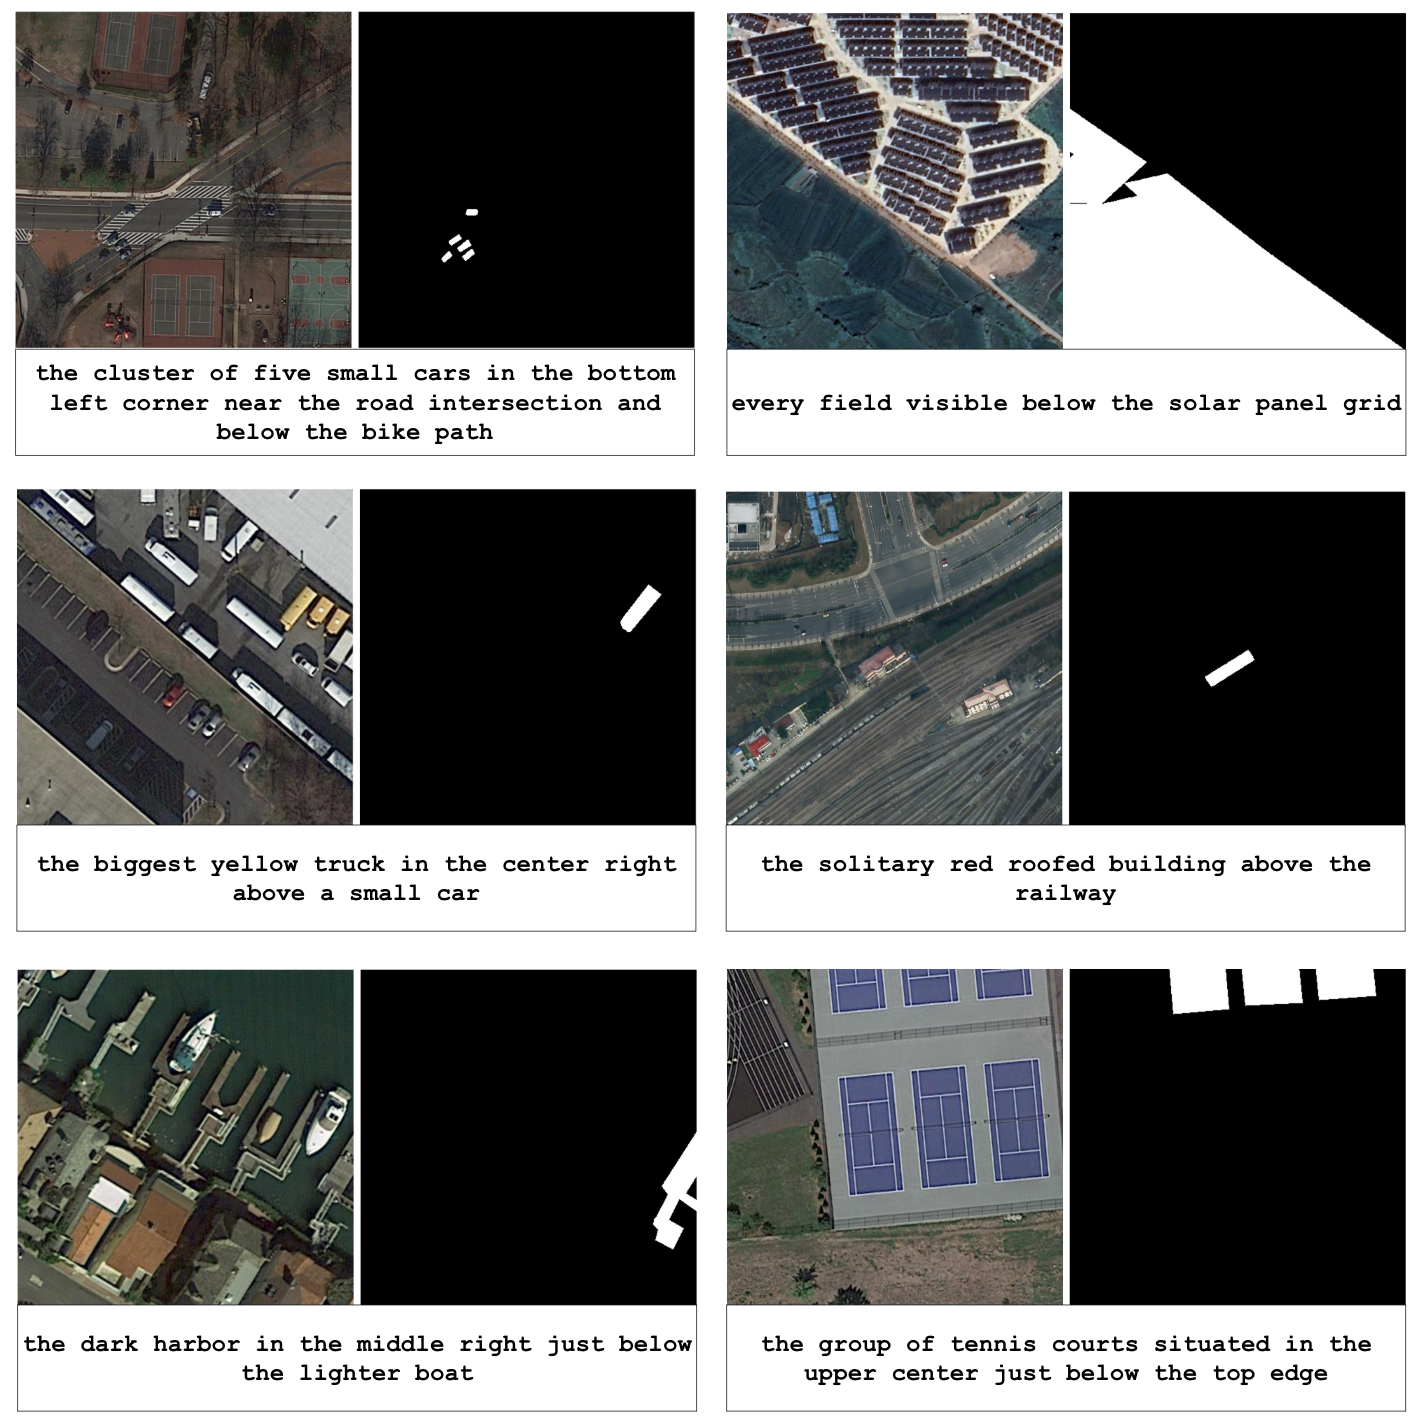
\includegraphics[width=\textwidth]{Images/6samples.png}
\caption{Representative examples from Aerial-D dataset showing diverse referring expressions with corresponding aerial images and ground truth masks.}
\label{fig:dataset_examples_intro}
\end{figure}

% #############################################################################
\section{Contributions}

The key contributions of this work include: (1) a comprehensive toolchain that enables the production of complex referring expression datasets from instance/semantic segmentation datasets, including a rule-based pipeline, Large Language Model enhancement and distillation methods, and historic image data augmentation with dedicated filtering; (2) the construction of Aerial-D, a dataset comprising over 1.5 million expressions across 37,288 aerial image patches, created entirely through the proposed automatic pipeline; and (3) a unified model trained on Aerial-D alongside four additional datasets, leveraging historic transformations and other applicable components of the toolchain across the training data to deliver referring expression segmentation over instances, groups, classes, and land cover regions while maintaining reliable performance on degraded historic imagery typical of archival aerial surveys.
% #############################################################################
\section{Document Structure}

This thesis is organized into six chapters and one appendix, each addressing distinct aspects of the methodology and evaluation:

\textbf{Chapter 2: Fundamental Concepts} establishes the theoretical foundation by introducing neural networks and deep learning principles, transformer architectures, computer vision fundamentals for image segmentation, and vision-language models. This chapter covers essential background on CLIP models, large language models, and the intersection of computer vision and natural language processing that enables referring segmentation.

\textbf{Chapter 3: Related Work} provides a comprehensive review of existing research in aerial image segmentation datasets, ranging from traditional semantic and instance segmentation datasets to specialized referring segmentation benchmarks. The chapter examines vision backbones for segmentation tasks, state-of-the-art referring segmentation models, and the emerging application of large language models to computer vision problems.

\textbf{Chapter 4: Aerial-D Dataset Construction} presents the systematic methodology for constructing the Aerial-D dataset. The chapter details the source datasets (iSAID~\cite{zamir2019isaid} and LoveDA~\cite{wang2021loveda}), the rule-based expression generation pipeline that transforms instance and semantic masks into referring expressions, LLM-based enhancement techniques using Gemma3, model distillation approaches, and comprehensive dataset statistics demonstrating the scale and diversity of the final resource.

\textbf{Chapter 5: Experiments} describes the experimental evaluation of the proposed approach using the RSRefSeg model architecture. The chapter covers the model implementation details, experimental setup across multiple benchmarks, comprehensive results on Aerial-D and comparison datasets including RRSIS-D, NWPU-Refer, RefSegRS, and Urban1960SatSeg, and ablation studies analyzing the contribution of different dataset enhancement components.

\textbf{Chapter 6: Conclusion and Future Work} synthesizes the key findings and contributions of this research while identifying promising directions for future investigation. The chapter summarizes the effectiveness of the automated dataset generation approach, discusses the implications for aerial image analysis, and outlines potential extensions to other remote sensing applications.

\textbf{Appendix A: LLM Enhancement Prompt} contains the complete system and user prompts employed during the Gemma3-based enhancement phase of dataset construction, providing full transparency and reproducibility for the LLM annotation process.
% If Printing on DOUBLE SIDED pages, the second page should be white.
% Otherwise, comment the following command:
\cleardoublepage
%
%Chapter 2
% #############################################################################
% This is Chapter 2
% !TEX root = ../main.tex
% #############################################################################
% Change the Name of the Chapter i the following line
\fancychapter{Fundamental Concepts}
\cleardoublepage
% The following line allows to ref this chapter
\label{chap:back}

This chapter introduces the fundamental technical concepts and architectures underlying open-vocabulary referring segmentation systems. We begin with neural networks and deep learning fundamentals (Section~2.1), then review attention and the transformer architecture (Section~2.2). We next summarize how transformers have been adapted for computer vision (Section~2.3), followed by image segmentation variants (Section~2.4) and vision-language foundations relevant to referring segmentation (Section~2.5).

% #############################################################################
\section{Neural Networks and Deep Learning}

Neural networks form the foundation of modern deep learning systems, providing the computational framework for learning complex patterns from data. The perceptron represents the simplest form of artificial neural network, consisting of a single computational unit that performs a linear combination of inputs followed by a nonlinear activation function, as illustrated in Figure~\ref{fig:perceptron}. For a perceptron with $N$ input features $\mathbf{x} = [x_1, x_2, \ldots, x_N]^T$, the output $y$ is computed as:

\begin{equation}
y = f(\mathbf{w}^T\mathbf{x} + b),
\end{equation}

where $\mathbf{w} = [w_1, w_2, \ldots, w_N]^T$ represents the weight vector, $b$ is the bias term, and $f(\cdot)$ denotes the activation function. This can be expanded as:

\begin{equation}
y = f\left(\sum_{i=1}^{N} w_i x_i + b\right).
\end{equation}

The activation function $f(\cdot)$ introduces nonlinearity into the model, enabling the perceptron to learn complex decision boundaries. Common activation functions include the sigmoid function $f(z) = \frac{1}{1 + e^{-z}}$, the hyperbolic tangent $f(z) = \tanh(z)$, and the rectified linear unit (ReLU) $f(z) = \max(0, z)$.

Multi-layer perceptrons extend the single perceptron by connecting multiple layers of neurons in a feedforward architecture, as shown in Figure~\ref{fig:mlp}. For a neural network with $L$ layers, where layer $l$ contains $n_l$ neurons, the forward propagation process computes:

\begin{equation}
\mathbf{a}^{(l)} = f^{(l)}\left(\mathbf{W}^{(l)}\mathbf{a}^{(l-1)} + \mathbf{b}^{(l)}\right),
\end{equation}

where $\mathbf{a}^{(l)}$ represents the activation vector of layer $l$, $\mathbf{W}^{(l)} \in \mathbb{R}^{n_l \times n_{l-1}}$ is the weight matrix connecting layers $l-1$ and $l$, $\mathbf{b}^{(l)} \in \mathbb{R}^{n_l}$ is the bias vector, and $f^{(l)}(\cdot)$ is the activation function for layer $l$. The universal approximation theorem demonstrates that multi-layer perceptrons with sufficient hidden units can approximate any continuous function on compact subsets of $\mathbb{R}^n$, providing the theoretical foundation for their expressiveness.

Neural networks are trained through gradient-based optimization methods that minimize a loss function $\mathcal{L}(\theta)$, where $\theta$ represents all learnable parameters. The loss function quantifies the difference between predicted outputs and ground truth targets, such as the mean squared error for regression tasks:

\begin{equation}
\mathcal{L}(\theta) = \frac{1}{n}\sum_{i=1}^{n}(y_i - \hat{y}_i)^2,
\end{equation}

where $n$ is the number of training samples, $y_i$ are the true labels, and $\hat{y}_i$ are the predicted outputs. The backpropagation algorithm efficiently computes gradients by applying the chain rule of calculus. The most common optimization algorithm is stochastic gradient descent, which updates parameters according to:

\begin{equation}
\theta_{t+1} = \theta_t - \eta \nabla_\theta \mathcal{L}(\theta_t),
\end{equation}

where $\eta$ is the learning rate and $\nabla_\theta \mathcal{L}(\theta_t)$ represents the gradient of the loss function with respect to parameters at iteration $t$.

\begin{figure}[t]
\centering
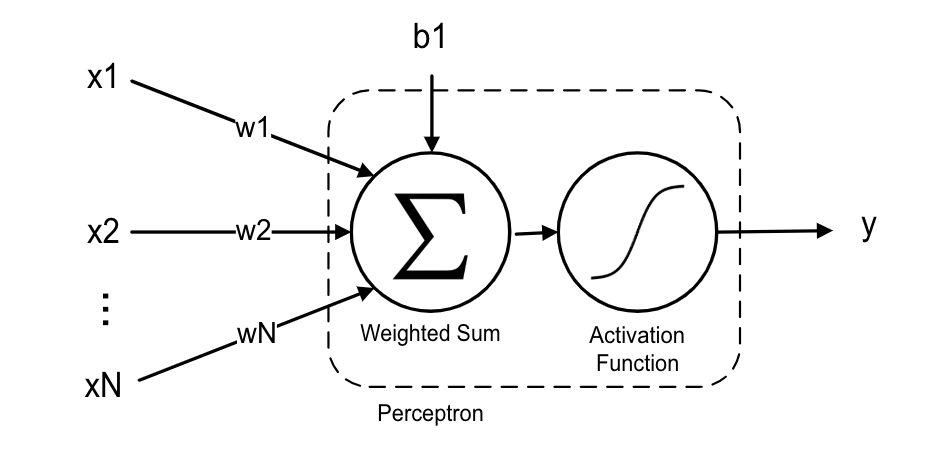
\includegraphics[width=0.6\textwidth]{Images/perceptron.png}
\caption{Perceptron architecture and basic neural network building block with inputs $x_1, x_2, \ldots, x_N$ and weights $w_1, \ldots, w_N$.}
\label{fig:perceptron}
\end{figure}

\begin{figure}[htbp]
\centering
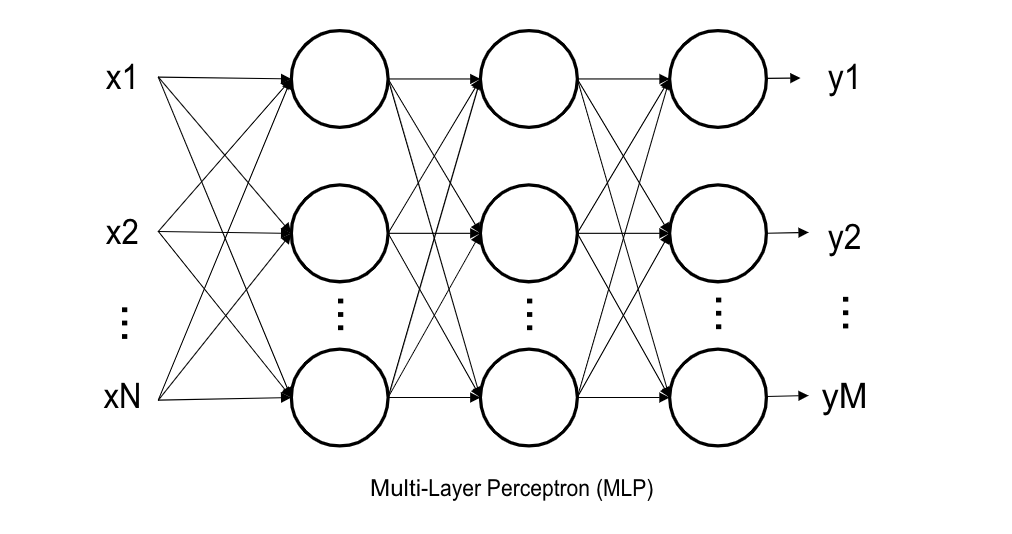
\includegraphics[width=0.6\textwidth]{Images/mlp.png}
\caption{Multi-layer perceptron architecture showing feedforward neural network structure operating on feature inputs $x_1, x_2, \ldots, x_N$.}
\label{fig:mlp}
\end{figure}

% #############################################################################
\section{Attention and Transformers}

The transformer architecture revolutionized sequence modeling by introducing a self-attention mechanism that enables models to process variable-length sequences more effectively than traditional fixed-size approaches. Unlike multi-layer perceptrons that operate on fixed-dimensional inputs, transformers can handle sequences of arbitrary length and are particularly effective at capturing long-range dependencies in medium to long sequences through the self-attention mechanism, making them suitable for tasks across multiple modalities including natural language, vision, audio, time series, or any sequential data where relationships between distant elements are important.

The core innovation of transformers lies in the self-attention mechanism, which allows each element in a sequence to attend to all other elements simultaneously, as illustrated in Figure~\ref{fig:transformer}. For a sequence of input tokens represented as embeddings $\mathbf{X} = [\mathbf{x}_1, \mathbf{x}_2, \ldots, \mathbf{x}_n] \in \mathbb{R}^{n \times d}$, where $n$ is the sequence length and $d$ is the embedding dimension, the self-attention mechanism computes three matrices: queries ($\mathbf{Q}$), keys ($\mathbf{K}$), and values ($\mathbf{V}$):

\begin{equation}
\mathbf{Q} = \mathbf{X}\mathbf{W}_Q, \quad \mathbf{K} = \mathbf{X}\mathbf{W}_K, \quad \mathbf{V} = \mathbf{X}\mathbf{W}_V,
\end{equation}

where $\mathbf{W}_Q, \mathbf{W}_K, \mathbf{W}_V \in \mathbb{R}^{d \times d_k}$ are learned parameter matrices. The attention scores $\boldsymbol{\alpha}$ are computed as:

\begin{equation}
\boldsymbol{\alpha} = \text{softmax}\left(\frac{\mathbf{Q}\mathbf{K}^T}{\sqrt{d_k}}\right),
\end{equation}

where the scaling factor $\sqrt{d_k}$ prevents the softmax function from saturating for large embedding dimensions. The final attention output is then computed as:

\begin{equation}
\text{Attention}(\mathbf{Q}, \mathbf{K}, \mathbf{V}) = \boldsymbol{\alpha}\mathbf{V},
\end{equation}

where $\boldsymbol{\alpha}$ represents the attention weights that determine how much each value $\mathbf{V}$ contributes to the output.

Since transformers process all positions in parallel, they lack inherent positional information. To address this, positional encodings are added to input embeddings to provide the model with information about token positions. The original transformer uses sinusoidal positional encodings:

\begin{equation}
PE_{(pos, 2i)} = \sin\left(\frac{pos}{10000^{2i/d}}\right), \quad PE_{(pos, 2i+1)} = \cos\left(\frac{pos}{10000^{2i/d}}\right),
\end{equation}

where $pos$ is the position index and $i$ is the dimension index. This encoding scheme allows the model to learn relative positions and generalizes to sequences longer than those seen during training.

The transformer block combines self-attention with feed-forward layers and residual connections. Each block applies layer normalization before both the attention and feed-forward operations, following the pre-normalization variant. The complete transformation for a single transformer block can be expressed as:

\begin{equation}
\mathbf{H}' = \text{Attention}(\text{LayerNorm}(\mathbf{H})) + \mathbf{H},
\end{equation}

\begin{equation}
\mathbf{H}'' = \text{FFN}(\text{LayerNorm}(\mathbf{H}')) + \mathbf{H}',
\end{equation}

where $\mathbf{H}$ represents the input hidden states and FFN denotes the feed-forward network. Multiple transformer blocks can be stacked to create deeper models that capture increasingly complex patterns in the input sequences. The output token embeddings from the final transformer layer can then be used for downstream tasks by attaching task-specific heads, such as classification layers for sentiment analysis or language modeling heads for text generation.

\begin{figure}[tb]
\centering
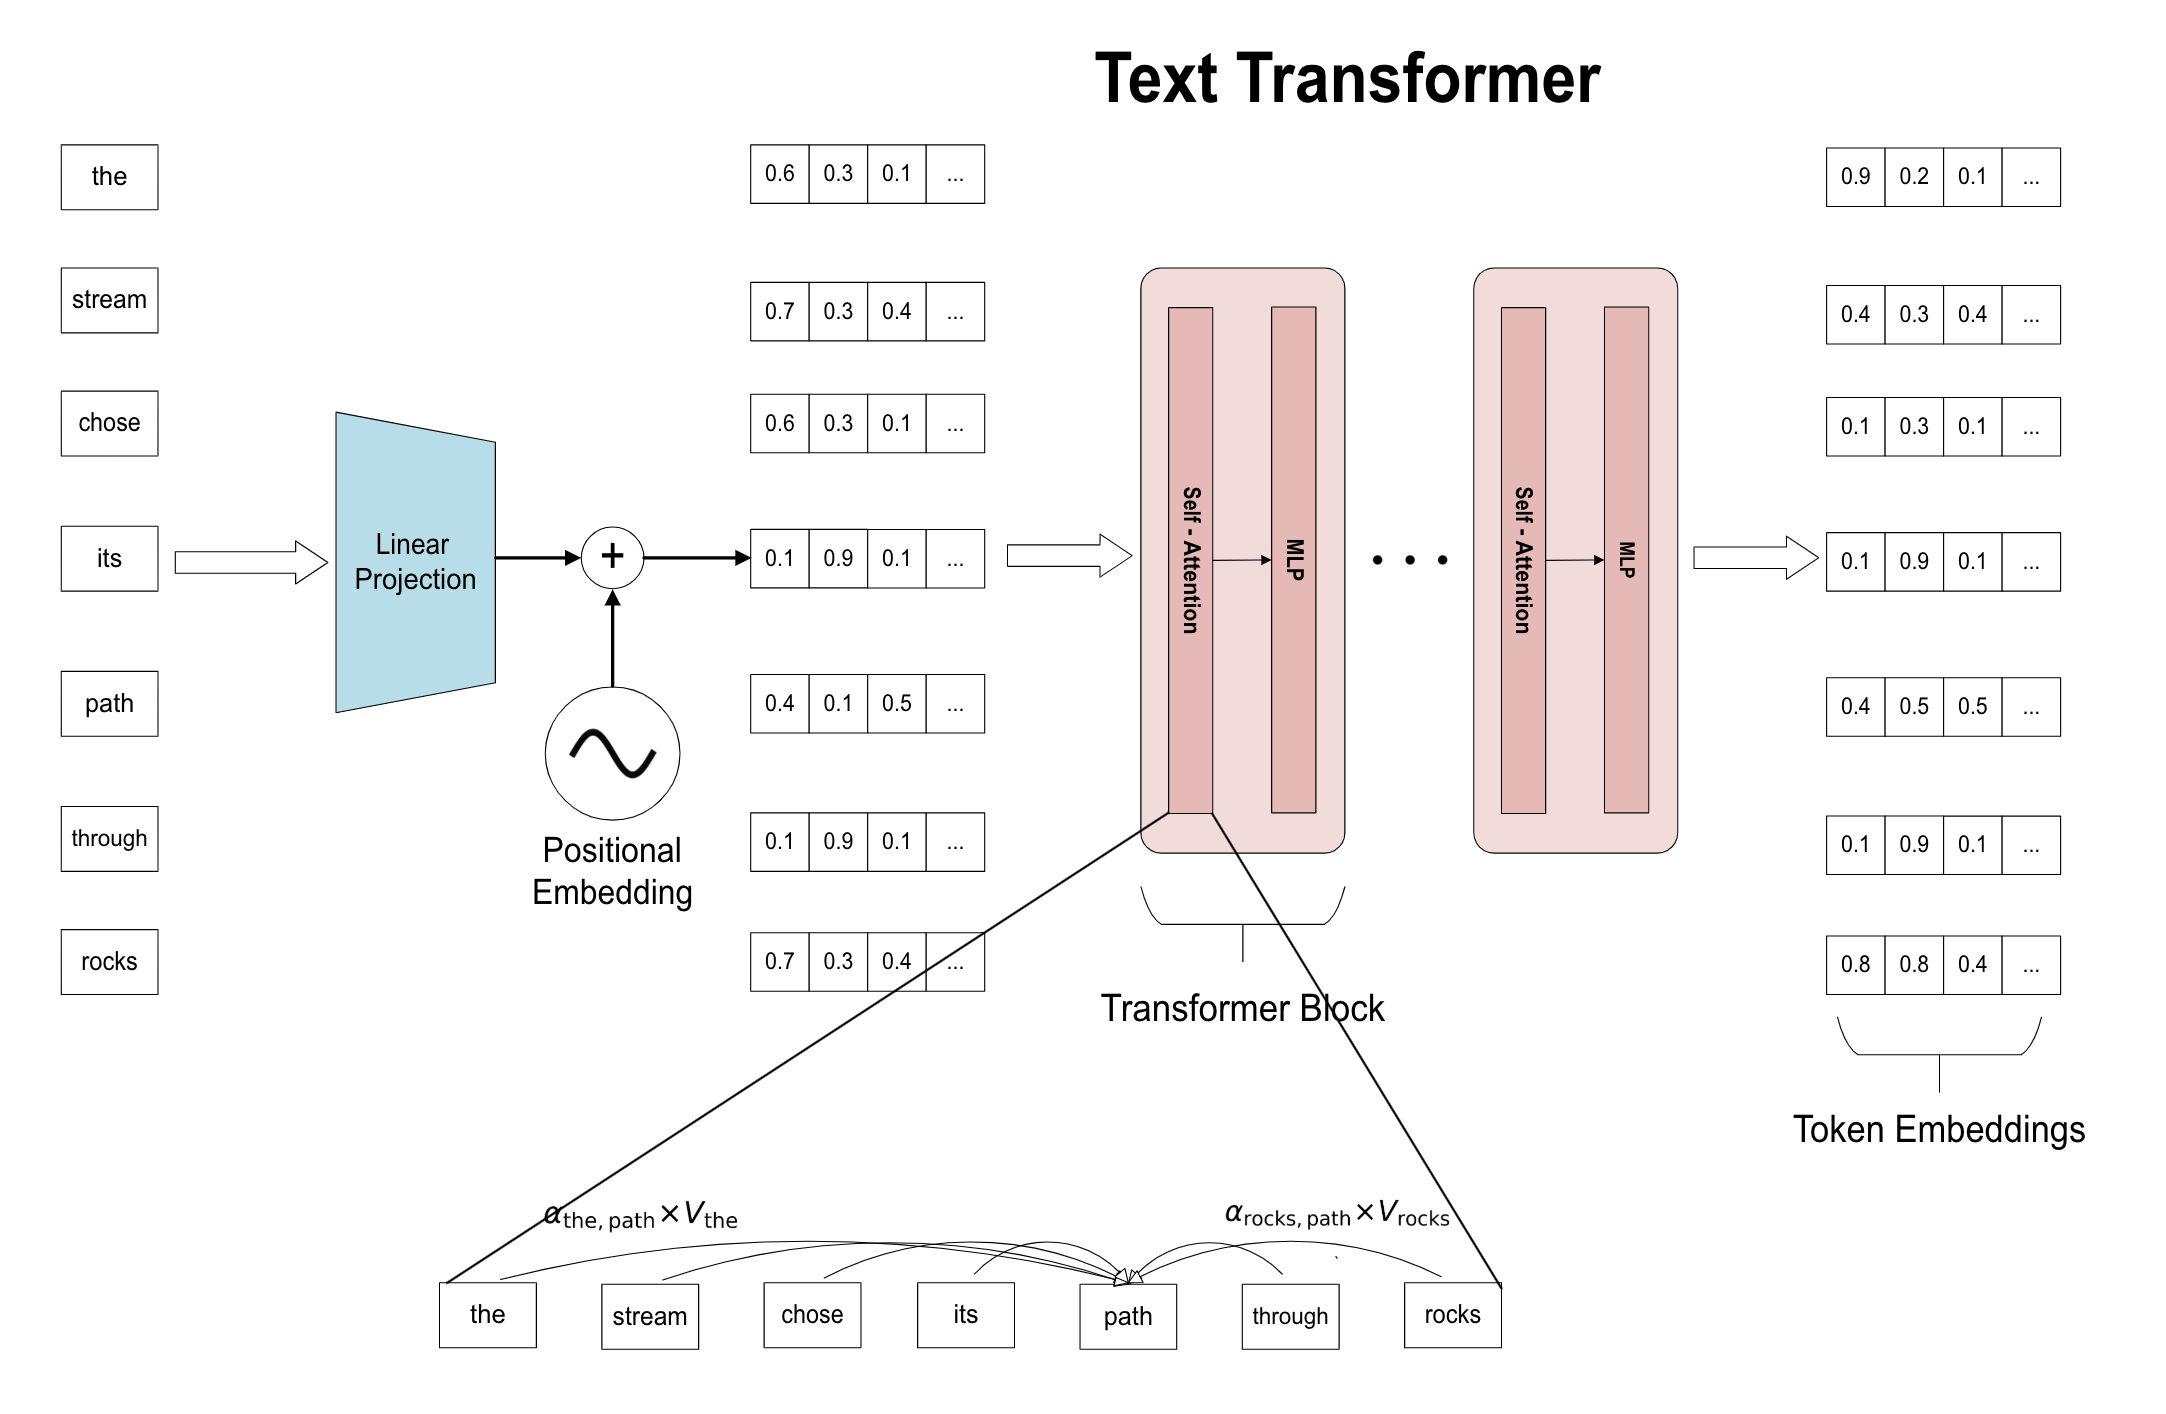
\includegraphics[width=0.9\textwidth]{Images/transformer.png}
\caption{Self-attention mechanism in transformers. The diagram shows how attention scores $\alpha$ are computed for each token, with specific examples of attention weights for tokens "path" and "rocks" relative to other words in the sequence "the stream chose its path through rocks".}
\label{fig:transformer}
\end{figure}

% #############################################################################
\section{Transformers for Computer Vision}

The success of transformers in natural language processing led to their adaptation for computer vision tasks, demonstrating the versatility of the self-attention mechanism across different modalities. Vision Transformers (ViTs) extend the transformer architecture to images by treating image patches as sequences of tokens, similar to how text transformers process word sequences.

The Vision Transformer architecture begins by dividing an input image into fixed-size square patches, as illustrated in Figure~\ref{fig:vit}. For an image of size $H \times W \times C$, where $H$ and $W$ are the height and width, and $C$ is the number of channels, the image is divided into $N = \frac{HW}{P^2}$ patches of size $P \times P$. Each patch is then flattened and linearly projected to create patch embeddings:

\begin{equation}
\mathbf{x}_p^{(i)} = \text{Linear}(\text{Flatten}(\mathbf{I}_p^{(i)})),
\end{equation}

where $\mathbf{I}_p^{(i)}$ represents the $i$-th patch and $\mathbf{x}_p^{(i)} \in \mathbb{R}^D$ is the corresponding patch embedding with dimension $D$.

Similar to text transformers, positional embeddings are added to patch embeddings to preserve spatial information about the patch locations within the original image. The sequence of patch embeddings is then processed through standard transformer blocks, applying self-attention mechanisms to capture relationships between different spatial regions of the image. This approach allows the model to learn which parts of the image are most relevant for the given task, whether it be classification, object detection, or feature extraction.

The output patch embeddings from the final transformer layer provide rich spatial representations that can be utilized for various computer vision tasks by attaching appropriate task-specific heads, such as classification heads for image categorization or detection heads for object localization. The Vision Transformer demonstrates that the same architectural principles underlying text transformers can be successfully applied to visual data, reinforcing the universal applicability of self-attention mechanisms across multiple modalities including text, vision, and other sequential data types.

\begin{figure}[tb]
\centering
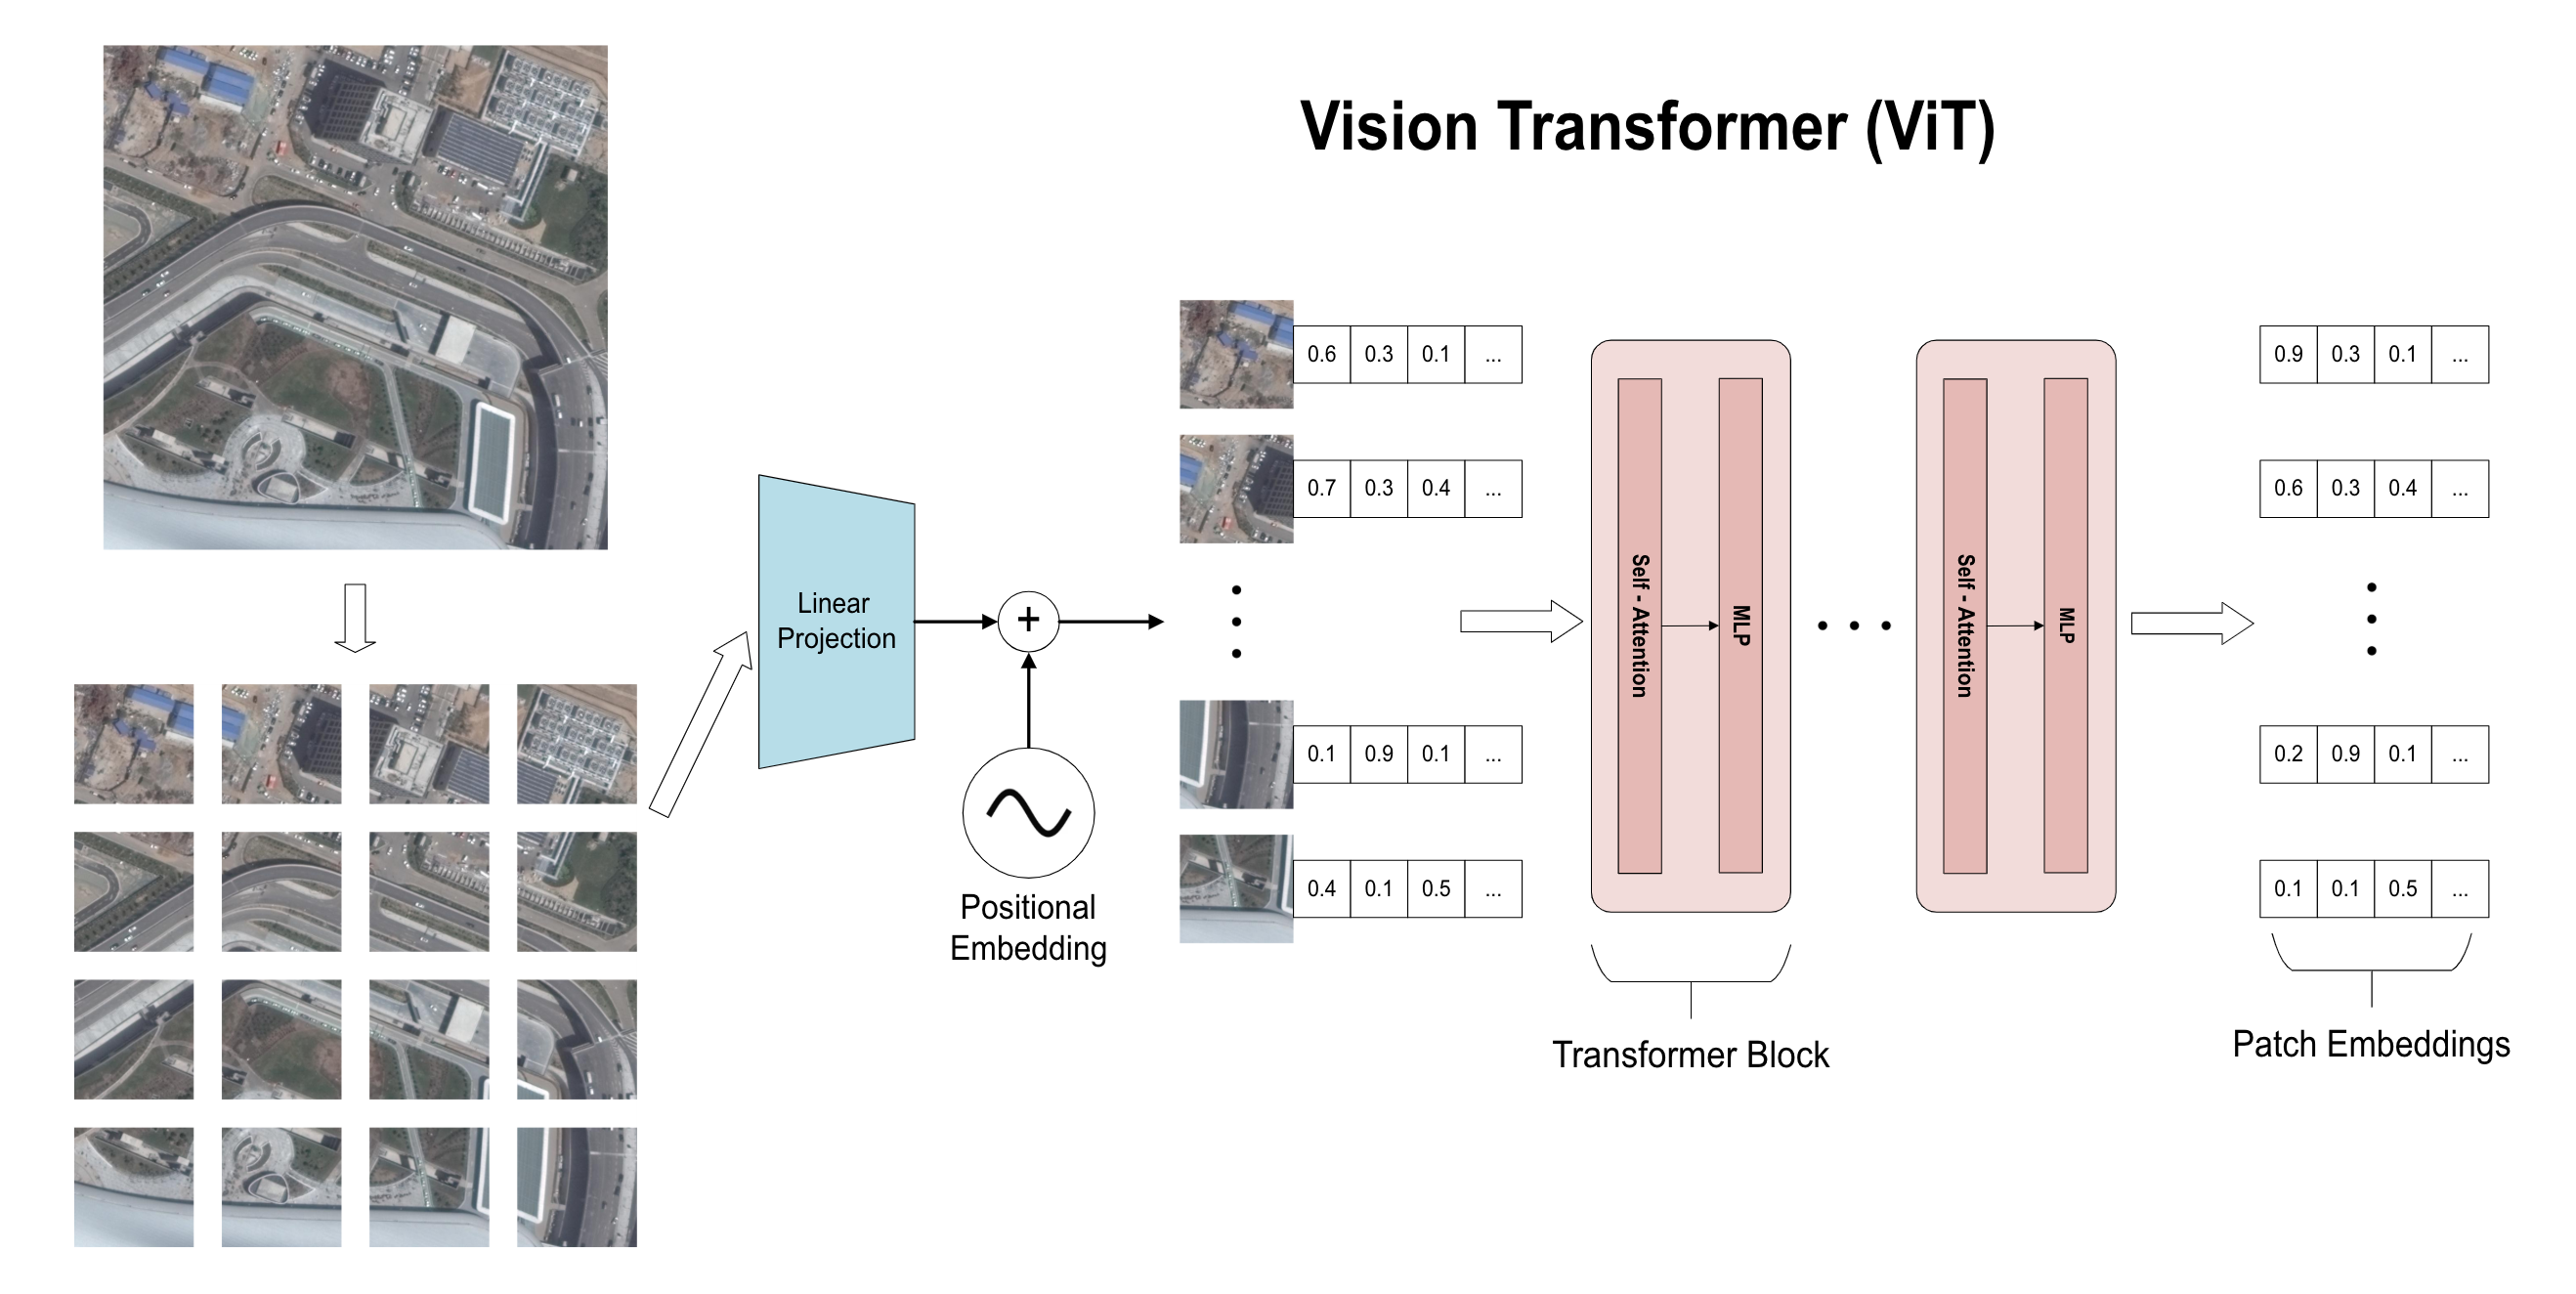
\includegraphics[width=0.9\textwidth]{Images/vit.png}
\caption{Vision Transformer (ViT) architecture for image classification and feature extraction. The input image is divided into square patches, which are then linearly projected and processed through transformer blocks, similar to how text transformers handle word tokens.}
\label{fig:vit}
\end{figure}


% #############################################################################
\section{Image Segmentation}

Image segmentation is a fundamental computer vision task that involves partitioning an image into semantically meaningful regions by classifying each pixel according to its content. At its core, segmentation can be viewed as a dense prediction problem where the model performs pixel-level binary or multi-class classification, determining for each spatial location whether it belongs to a particular object or region of interest.

The segmentation process transforms an input image $\mathbf{I} \in \mathbb{R}^{H \times W \times C}$ into a segmentation mask $\mathbf{M} \in \{0, 1\}^{H \times W}$ for binary segmentation, or $\mathbf{M} \in \{0, 1, \ldots, K\}^{H \times W}$ for multi-class segmentation with $K$ categories. Each pixel $(i, j)$ in the output mask $\mathbf{M}_{i,j}$ represents the predicted class label for the corresponding spatial location in the input image.

Different variations of the segmentation task address distinct aspects of scene understanding, as illustrated in Figure~\ref{fig:segmentation}. Semantic segmentation assigns each pixel to a predefined semantic category, such as "small vehicle," "large vehicle," or "plane," without distinguishing between individual object instances within the same category. This approach provides a comprehensive understanding of scene composition but treats all objects of the same class as a single entity.

Instance segmentation extends semantic segmentation by identifying and delineating individual object instances, enabling the model to distinguish between separate objects that belong to the same semantic category. For example, multiple aircraft in an aerial image would be segmented as distinct entities rather than merged into a single "plane" region. This capability is crucial for applications requiring precise object counting and individual object analysis.

Referring instance segmentation represents the most sophisticated variant, combining instance-level precision with natural language understanding. This task requires the model to segment a specific object instance based on a natural language description or prompt, such as "large vehicle in between two planes." The model must simultaneously understand the linguistic description and identify the corresponding visual region, bridging the gap between language and vision modalities. This approach enables more intuitive human-computer interaction and supports complex queries that cannot be addressed through traditional category-based segmentation methods.

\begin{figure}[htbp]
\centering
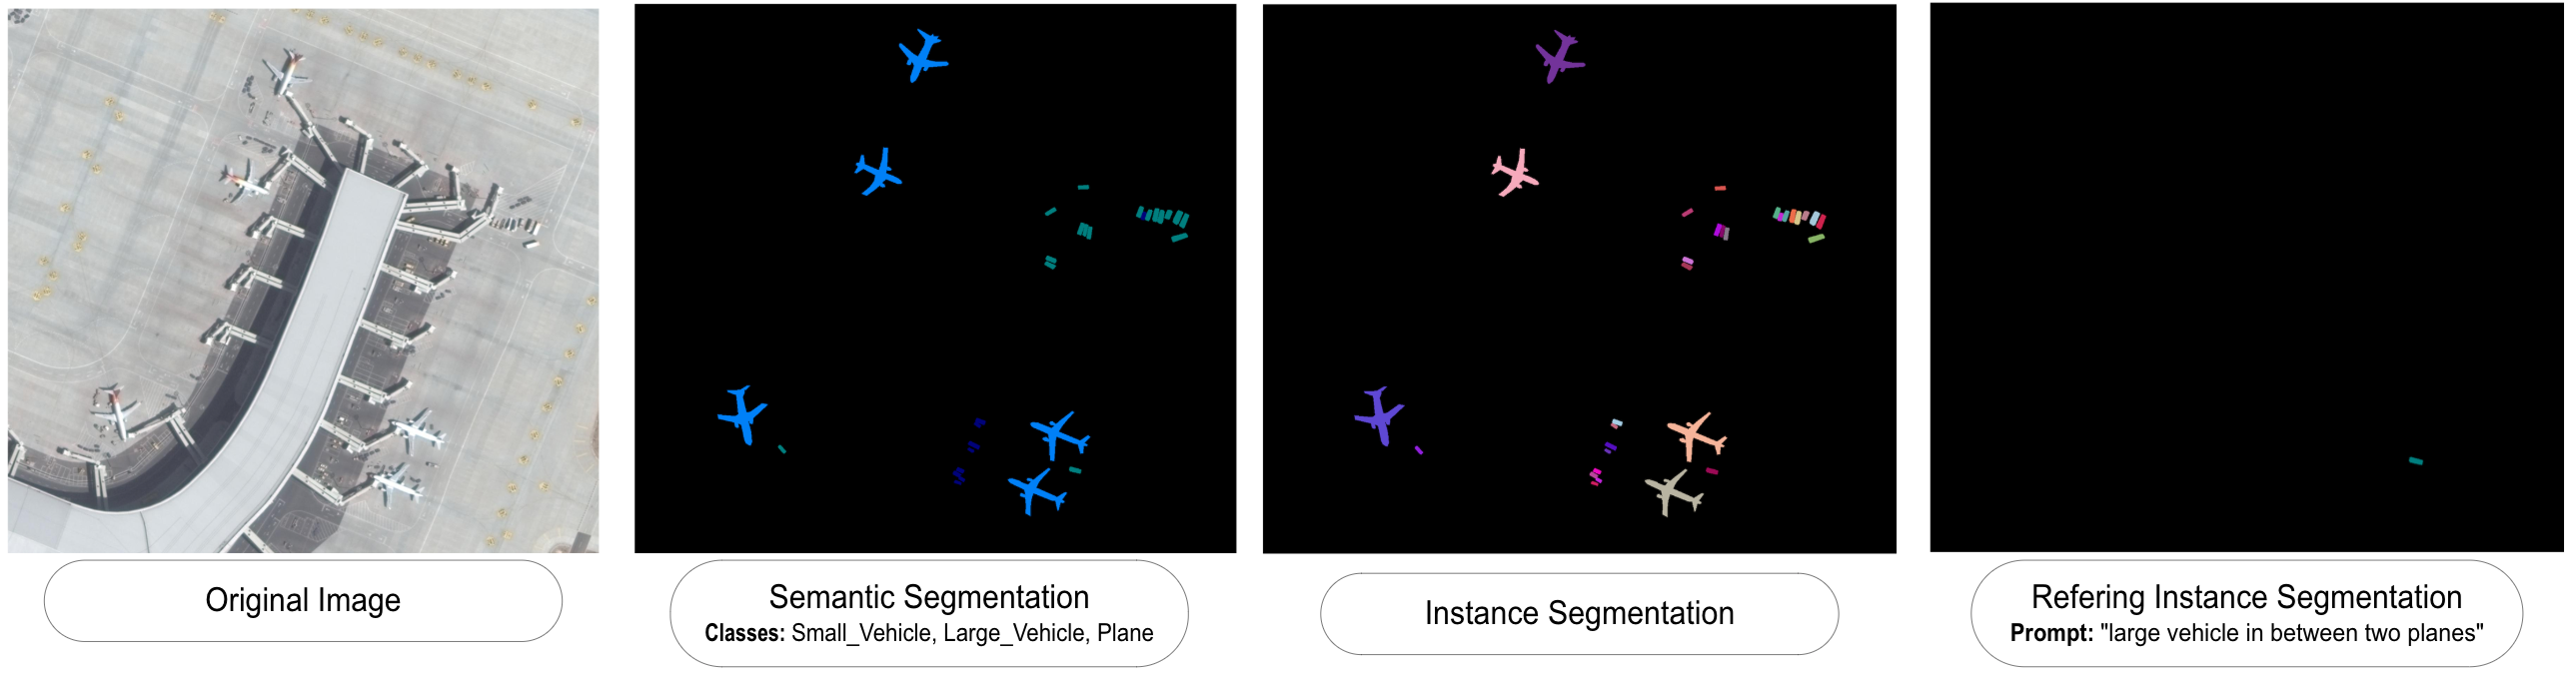
\includegraphics[width=1.0\textwidth]{Images/segmentation.png}
\caption{Comparison of segmentation types: semantic segmentation, instance segmentation, and referring instance segmentation with natural language prompts.}
\label{fig:segmentation}
\end{figure}

% #############################################################################
\section{Vision-Language Models}

Vision-language models represent a significant advancement in multimodal artificial intelligence, enabling systems to understand and reason about both visual and textual information simultaneously. These architectures bridge the gap between computer vision and natural language processing by learning joint representations that capture semantic relationships across modalities.

\subsection{CLIP and Visual-Language Learning}

Contrastive Language-Image Pre-training (CLIP) introduces a powerful framework for learning visual-textual representations through contrastive learning~\cite{clip}. The architecture consists of two separate transformer encoders: an image encoder that processes visual input and a text encoder that handles natural language descriptions, as illustrated in Figure~\ref{fig:clip_architecture}.

The core innovation of CLIP lies in its contrastive pre-training methodology, which learns to align image and text embeddings in a shared representation space. During training, the model processes batches of image-text pairs and computes similarity scores between all possible combinations. For a batch of $N$ image-text pairs, CLIP maximizes the cosine similarity between correct pairs while minimizing similarity between incorrect pairs:

\begin{equation}
\mathcal{L}_{\text{contrastive}} = -\frac{1}{N}\sum_{i=1}^{N} \left[ \log \frac{\exp(\text{sim}(\mathbf{I}_i, \mathbf{T}_i) / \tau)}{\sum_{j=1}^{N} \exp(\text{sim}(\mathbf{I}_i, \mathbf{T}_j) / \tau)} \right],
\end{equation}

where $\mathbf{I}_i$ and $\mathbf{T}_i$ represent image and text embeddings respectively, $\text{sim}(\cdot, \cdot)$ computes cosine similarity, and $\tau$ is a learned temperature parameter that controls the sharpness of the softmax distribution.

This contrastive objective enables CLIP to achieve remarkable zero-shot classification capabilities. Given a new image and a set of candidate class descriptions, the model can classify the image by computing similarities between the image embedding and text embeddings for each class description, selecting the class with the highest similarity score. This approach eliminates the need for task-specific fine-tuning and demonstrates strong generalization across diverse visual domains.

The learned joint embedding space has proven valuable for numerous downstream vision-language tasks beyond classification. The aligned representations enable applications such as image retrieval using text queries, caption generation, visual question answering, and multimodal reasoning tasks. The versatility of CLIP embeddings stems from their ability to capture semantic relationships that transfer across different tasks and domains, making them fundamental building blocks for modern multimodal systems.

\begin{figure}[htbp]
\centering
\subfigure[Contrastive pre-training methodology.]{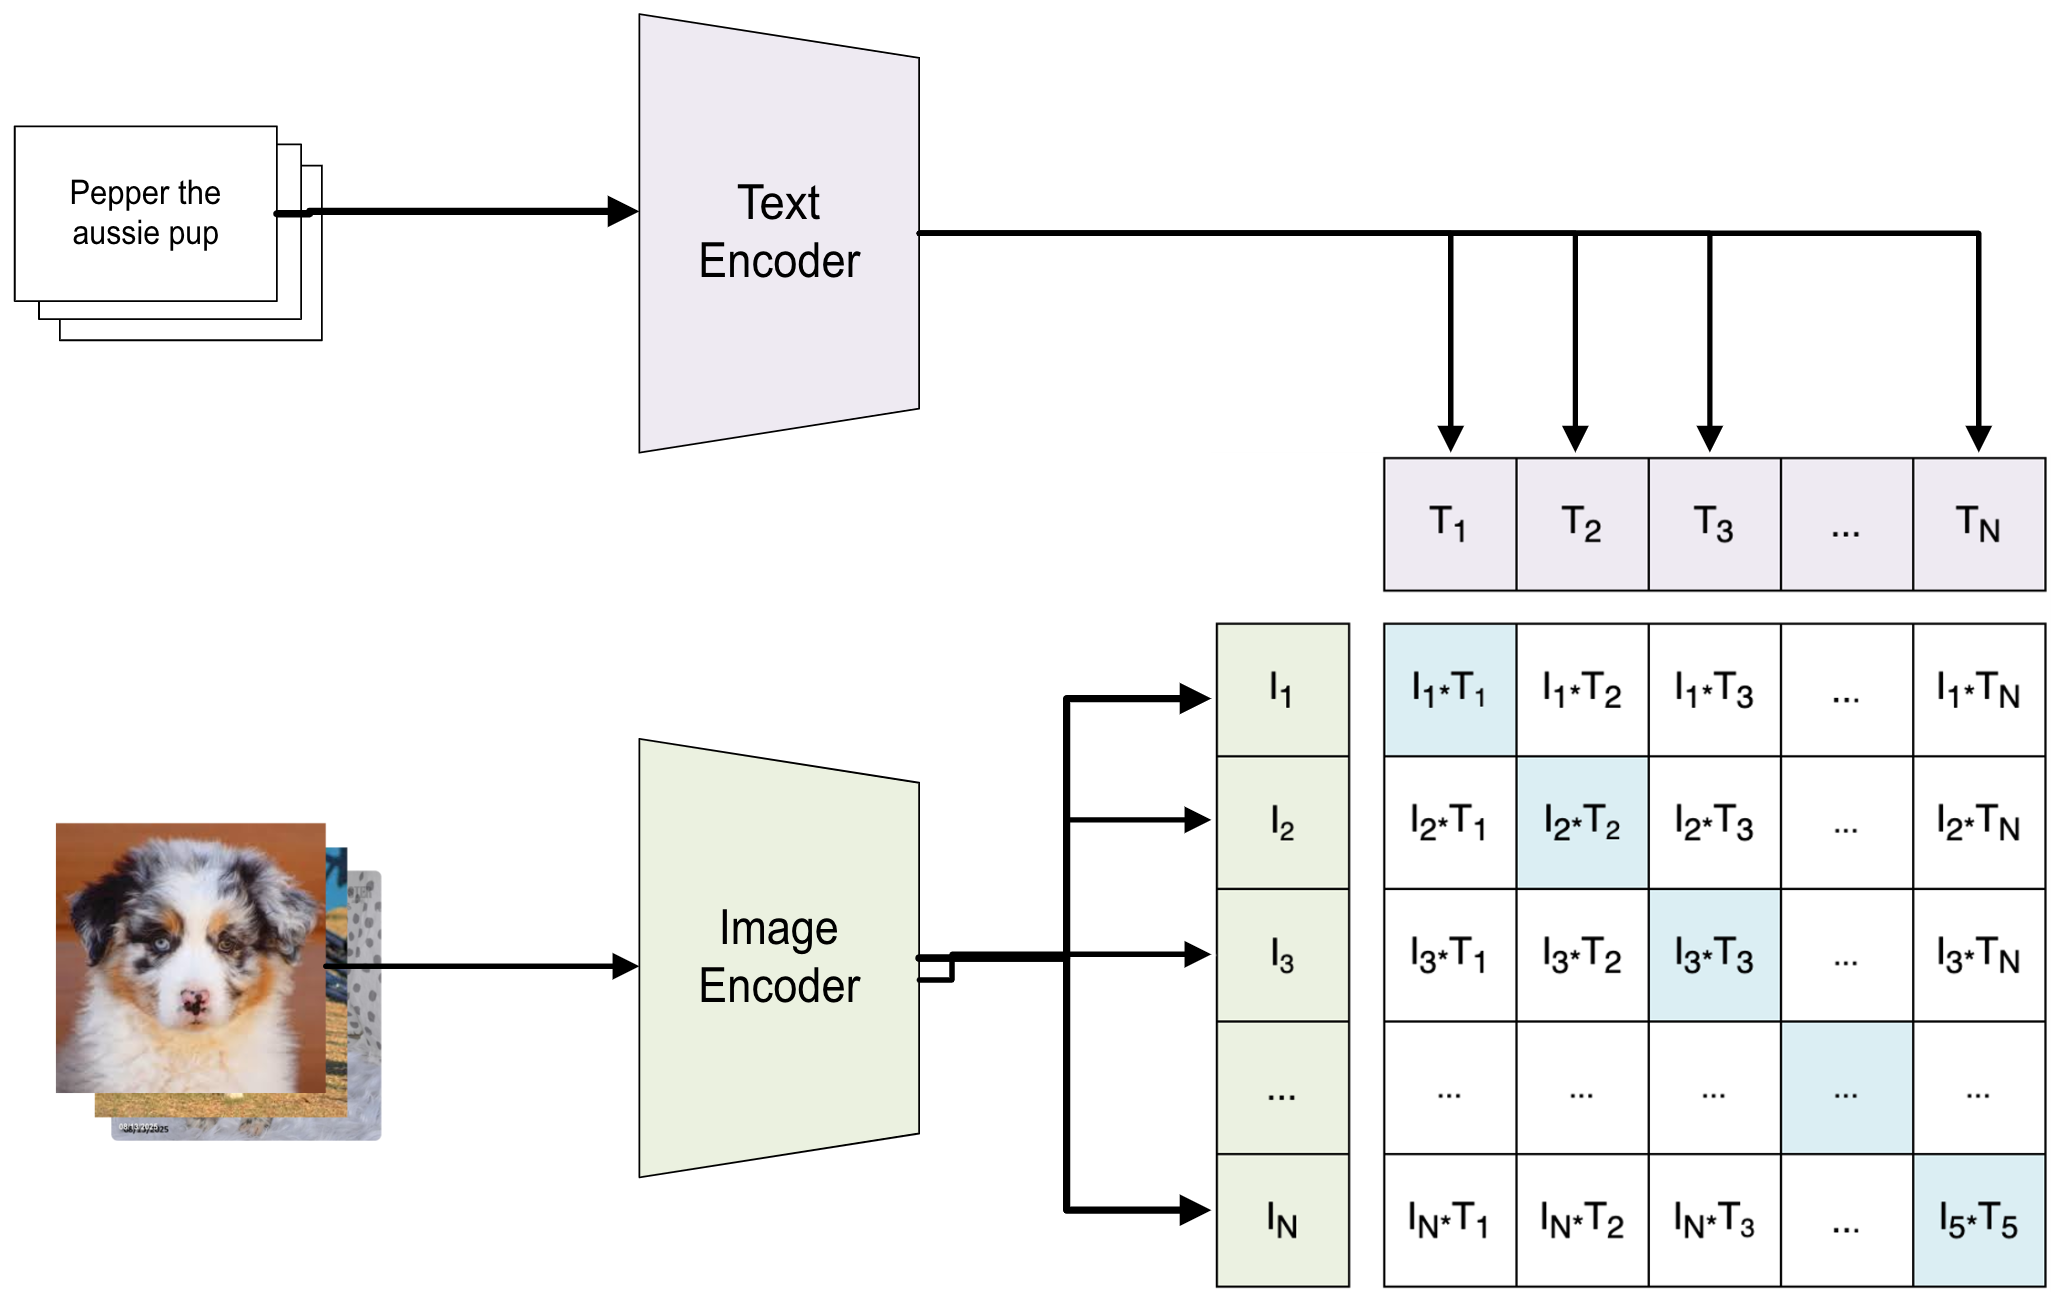
\includegraphics[width=0.45\textwidth]{Images/contrastive_pretraining.png}\label{fig:contrastive_pretraining}}
\hfill
\subfigure[Zero-shot prediction capabilities.]{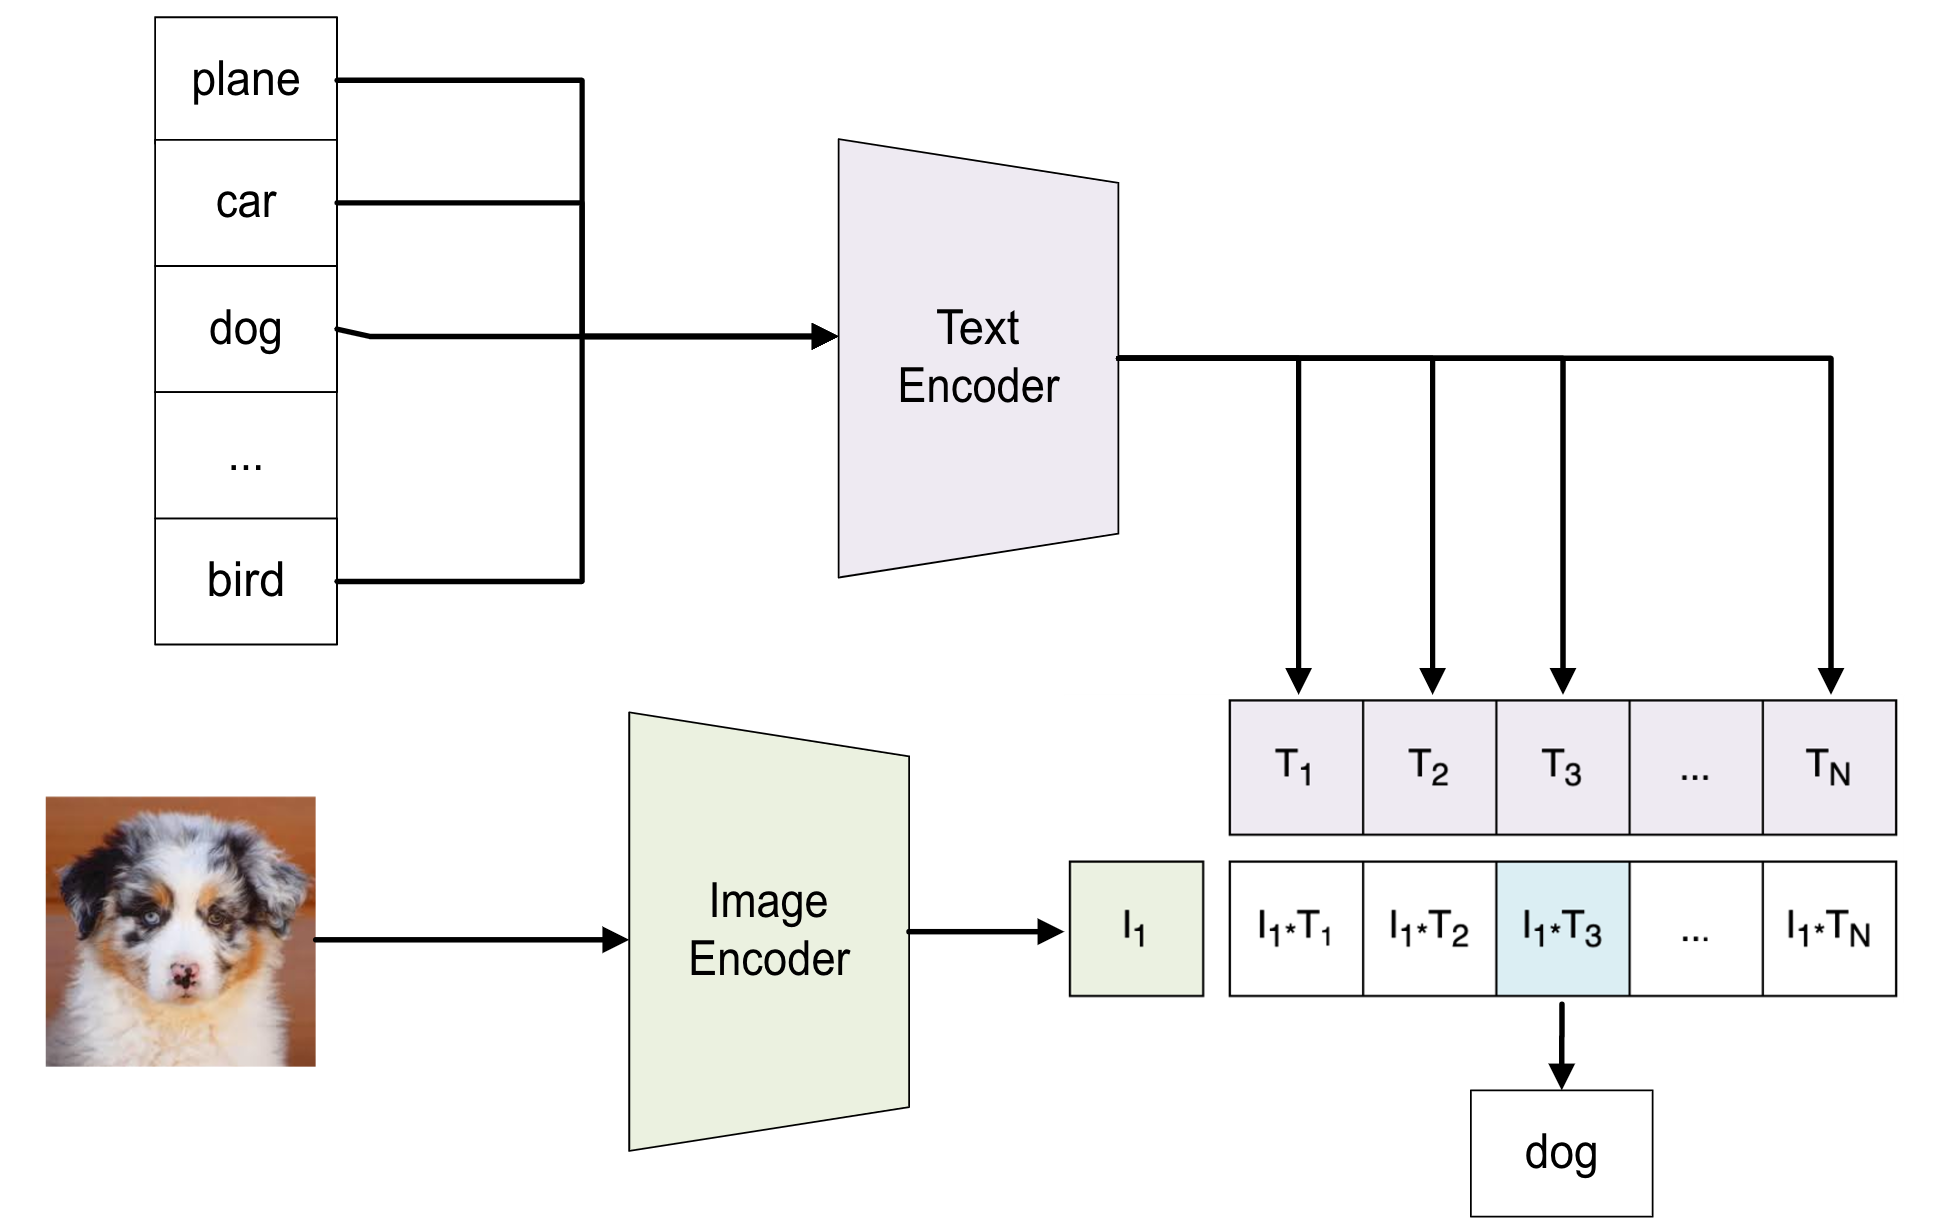
\includegraphics[width=0.45\textwidth]{Images/zero_shot_prediction.png}\label{fig:zero_shot_prediction}}
\caption{CLIP architecture components showing contrastive pre-training and zero-shot prediction mechanisms.}
\label{fig:clip_architecture}
\end{figure}

\subsection{Large Multimodal Language Models}

Large Language Models (LLMs) have emerged as powerful foundation models that demonstrate remarkable capabilities in natural language understanding, generation, and reasoning. These models, exemplified by the GPT (Generative Pre-trained Transformer) family, utilize transformer decoder architectures trained on vast text corpora to learn rich linguistic representations and world knowledge.

The GPT architecture employs a causal transformer decoder that generates text autoregressively, predicting the next token in a sequence based on all previous tokens, as illustrated in Figure~\ref{fig:gpt}. The diagram shows the characteristic feedback mechanism where each predicted token is fed back into the sequence for subsequent predictions. For a sequence of tokens $\mathbf{x} = [x_1, x_2, \ldots, x_t]$, the model processes the entire sequence through multiple transformer layers before computing the probability of the next token $x_{t+1}$ through an output MLP:

\begin{equation}
P(x_{t+1} | x_1, x_2, \ldots, x_t) = \text{softmax}(\mathbf{W}_o \mathbf{h}_t),
\end{equation}

where $\mathbf{h}_t$ represents the hidden state at position $t$ from the final transformer layer and $\mathbf{W}_o$ is the output projection matrix. The training objective maximizes the likelihood of the training sequences:

\begin{equation}
\mathcal{L}_{\text{LM}} = -\sum_{i=1}^{T} \log P(x_i | x_1, \ldots, x_{i-1}),
\end{equation}

where $T$ is the sequence length. This next-token prediction objective, demonstrated in the figure's "Add to sequence" feedback loop, enables LLMs to learn complex linguistic patterns, semantic relationships, and contextual dependencies from large-scale text data.

The versatility of the transformer architecture allows LLMs to process heterogeneous token sequences that extend beyond natural language. In multimodal contexts, the input sequence can include tokens from vision encoders, such as those produced by CLIP's image encoder. Since CLIP's visual representations are aligned with language through contrastive training, LLMs can be trained to understand these visual tokens alongside textual tokens, creating truly multimodal language models. This integration enables the model to process mixed sequences containing both visual and textual information, allowing for sophisticated capabilities such as visual question answering, image captioning with rich contextual descriptions, and instruction-following for complex visual tasks. The extensive world knowledge captured by LLMs during pre-training, combined with their ability to process visual tokens, allows them to provide contextual understanding that goes beyond simple pattern recognition, enabling more nuanced and informative multimodal interactions.

Modern implementations of large multimodal language models demonstrate remarkable capabilities in vision-language understanding and generation~\cite{gemma3,o3,gemini25}.

These systems integrate vision and language to enable multimodal capabilities~\cite{clip,siglip}.

Open-source models integrate vision encoders with transformer decoder architectures, enabling sophisticated multimodal reasoning while maintaining accessibility for research and development~\cite{gemma3,siglip,siglip2}.

Proprietary large-scale models represent the current state-of-the-art in multimodal language modeling, demonstrating advanced capabilities in complex visual reasoning, detailed image analysis, and sophisticated instruction following across multiple domains~\cite{o3}.

For example, OpenAI's o3 family~\cite{o3}.

Similarly, Google's Gemini 2.5~\cite{gemini25}.

These models leverage massive computational resources and extensive multimodal training datasets to achieve performance levels that approach human-level understanding in many vision-language tasks, setting new benchmarks for what is possible in artificial multimodal intelligence.

\begin{figure}[htbp]
\centering
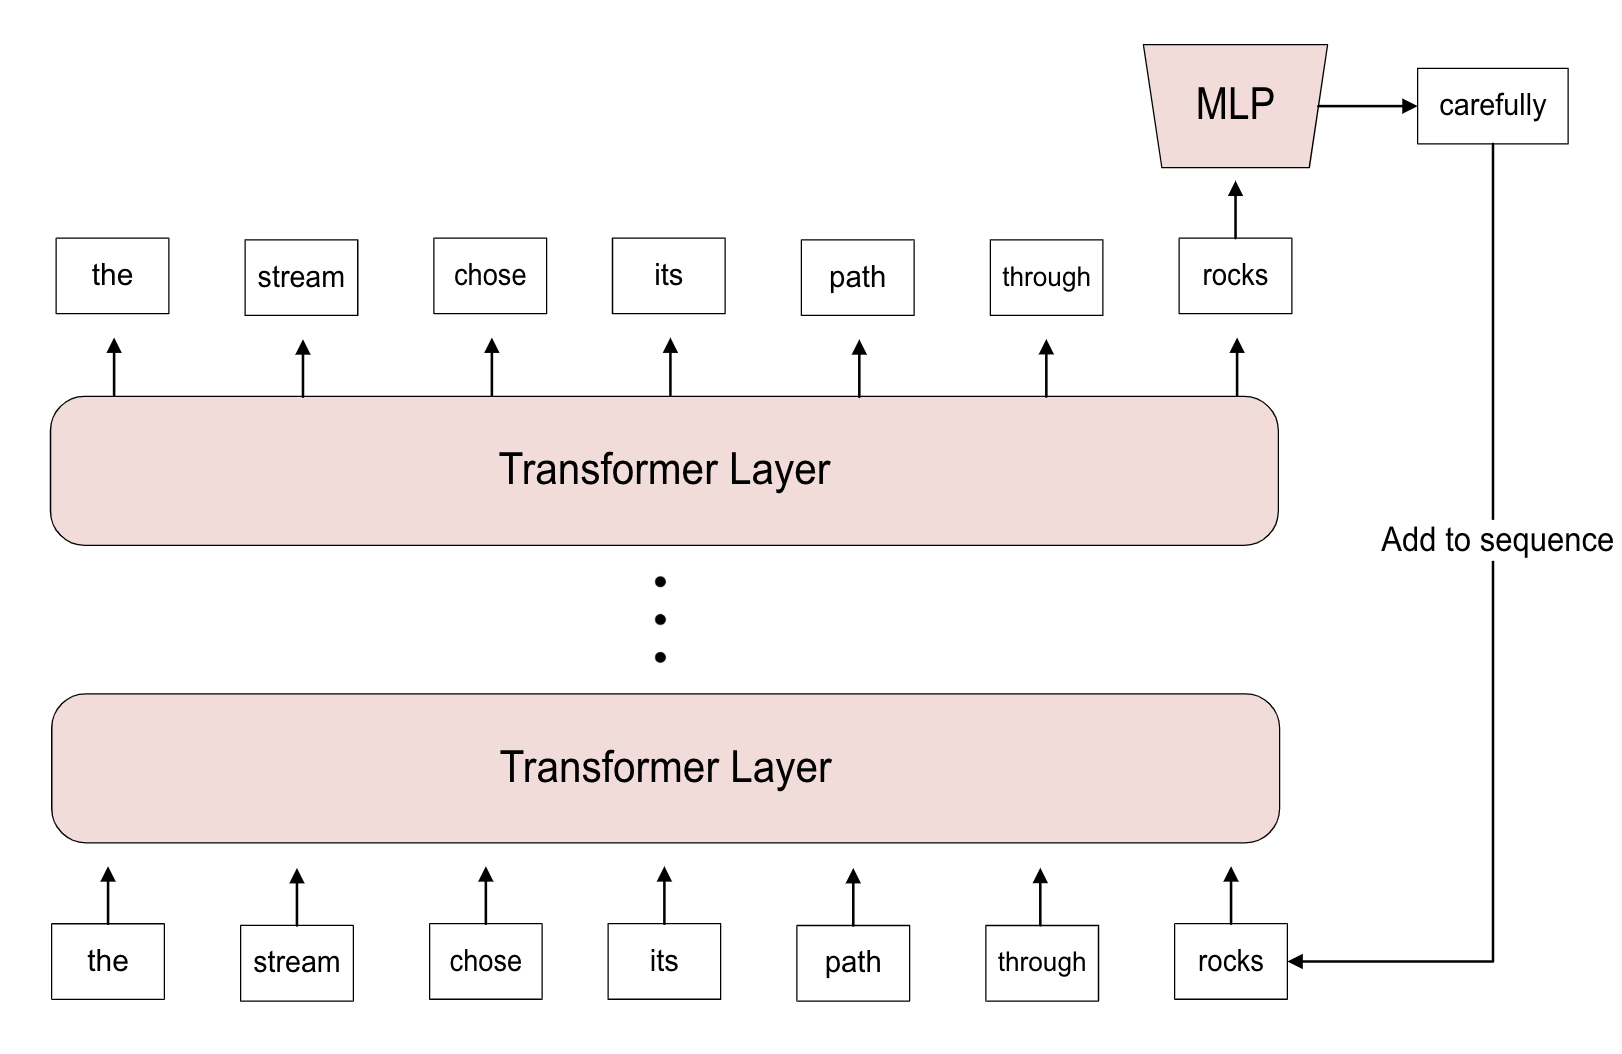
\includegraphics[width=0.8\textwidth]{Images/gpt.png}
\caption{GPT autoregressive language model architecture showing the transformer decoder stack with next-token prediction and feedback mechanism.}
\label{fig:gpt}
\end{figure}

% #############################################################################
\section{Overview}

This chapter has introduced the fundamental technical concepts that underpin modern open-vocabulary referring segmentation systems. Neural networks and deep learning provide the computational foundation through multi-layer perceptrons and gradient-based optimization, enabling the learning of complex patterns from data. The transformer architecture, with its self-attention mechanism, revolutionizes sequence modeling by allowing parallel processing and capturing long-range dependencies across different modalities.

The extension of transformers to computer vision through Vision Transformers demonstrates the versatility of attention mechanisms beyond natural language processing. By treating image patches as sequences, ViTs enable the processing of visual information using the same architectural principles that have proven successful for text, laying the groundwork for unified multimodal architectures.

Image segmentation represents a core computer vision task that partitions images into semantically meaningful regions through dense pixel-level prediction. The progression from semantic segmentation through instance segmentation to referring instance segmentation illustrates the evolution toward more sophisticated scene understanding capabilities that combine visual analysis with natural language comprehension.

Vision-language models, exemplified by CLIP, establish the crucial bridge between visual and textual modalities through contrastive learning approaches. By learning aligned representations across modalities, these models enable zero-shot capabilities and provide the foundation for multimodal understanding. Large multimodal language models further extend this concept by integrating visual tokens into autoregressive generation frameworks, enabling sophisticated reasoning about both textual and visual content.

Together, these fundamental concepts create a comprehensive technical foundation for open-vocabulary referring segmentation systems that can understand natural language descriptions and precisely segment corresponding visual regions in aerial imagery. The following chapters build upon these foundations to examine existing approaches and present novel contributions to this challenging problem domain.
% If Printing on DOUBLE SIDED pages, the second page should be white.
% Otherwise, comment the following command:
\cleardoublepage
%
%Chapter 3
% #############################################################################
% This is Chapter 3
% !TEX root = ../main.tex
% #############################################################################
% Change the Name of the Chapter i the following line
\fancychapter{Related Work}
\cleardoublepage
% The following line allows to ref this chapter
\label{chap:architecture}

This chapter reviews existing work in aerial image segmentation datasets, referring segmentation models, and related approaches.

% #############################################################################
\section{Aerial Image Segmentation Datasets}

Overview of datasets used for aerial imagery analysis and referring segmentation tasks.

[Reference to iSAID dataset] % \cite{placeholder_isaid}

\begin{figure}[htbp]
\centering
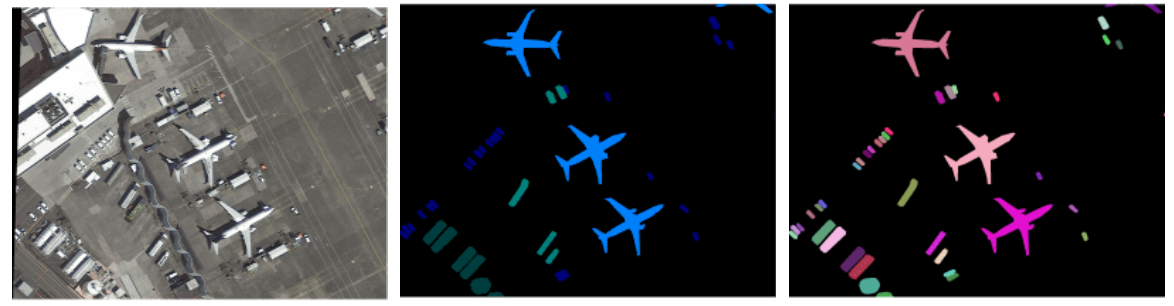
\includegraphics[width=0.8\textwidth]{Images/isaid_examples.png}
\caption{iSAID dataset examples showing instance segmentation and semantic segmentation annotations for aerial imagery.}
\label{fig:isaid_examples}
\end{figure}

[Reference to LoveDA dataset] % \cite{placeholder_loveda}

\begin{figure}[htbp]
\centering
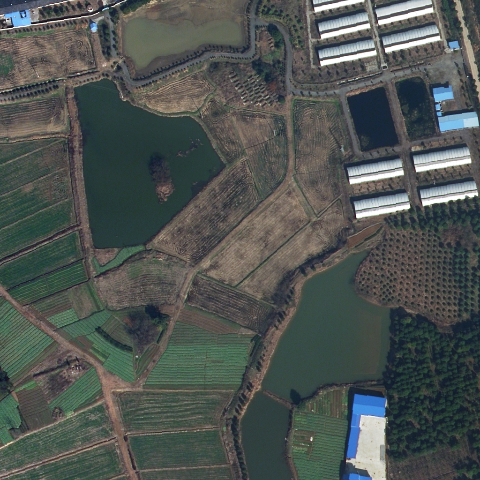
\includegraphics[width=0.8\textwidth]{Images/loveda.png}
\caption{LoveDA dataset examples showing semantic segmentation annotations for land use and land cover classification in aerial imagery.}
\label{fig:loveda_examples}
\end{figure}

[Reference to Potsdam and Vaihingen semantic segmentation datasets] % \cite{placeholder_potsdam} \cite{placeholder_vaihingen}

[Reference to RefSegRS referring segmentation dataset] % \cite{placeholder_refsegrs}

[Reference to RRSIS-D dataset] % \cite{placeholder_rrsis_d}

\begin{figure}[htbp]
\centering
\subfigure[RefSegRS dataset example samples.]{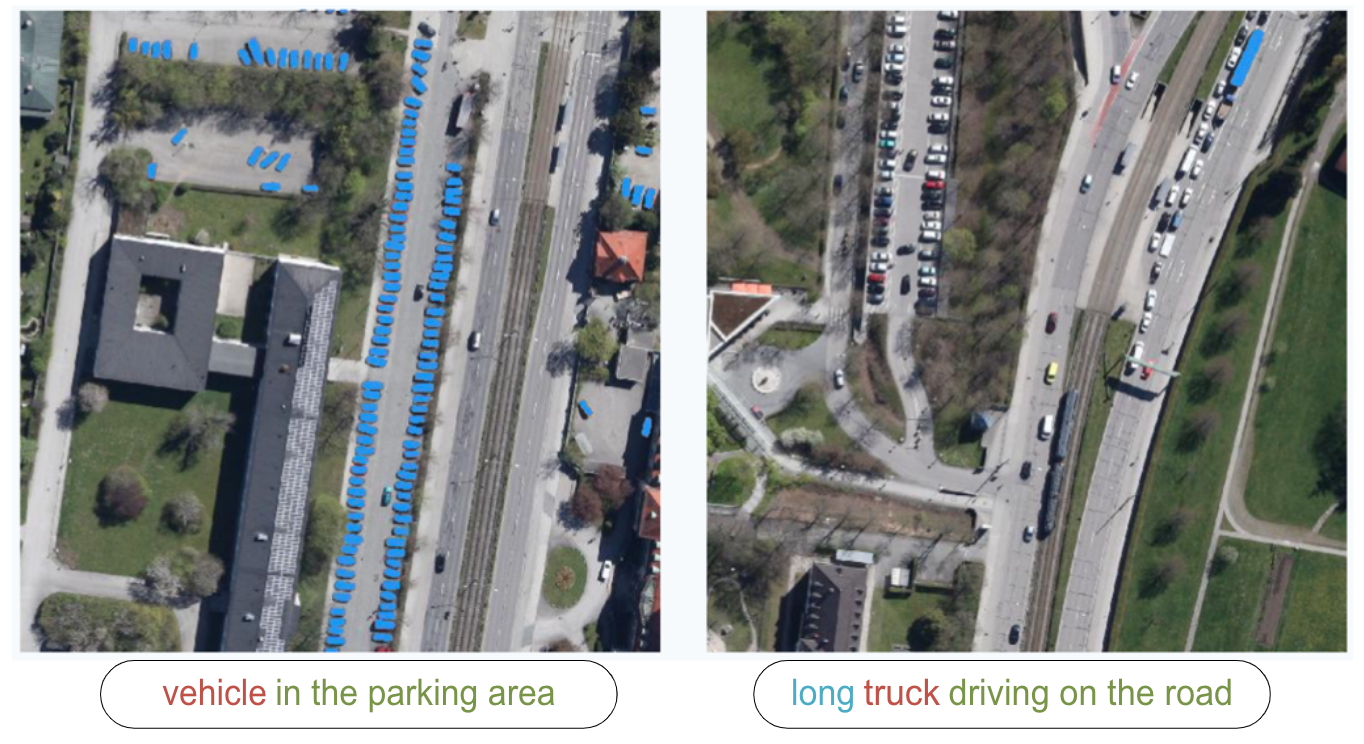
\includegraphics[width=0.45\textwidth]{Images/refsegrs.png}\label{fig:refsegrs}}
\hfill
\subfigure[RRSIS-D dataset example samples.]{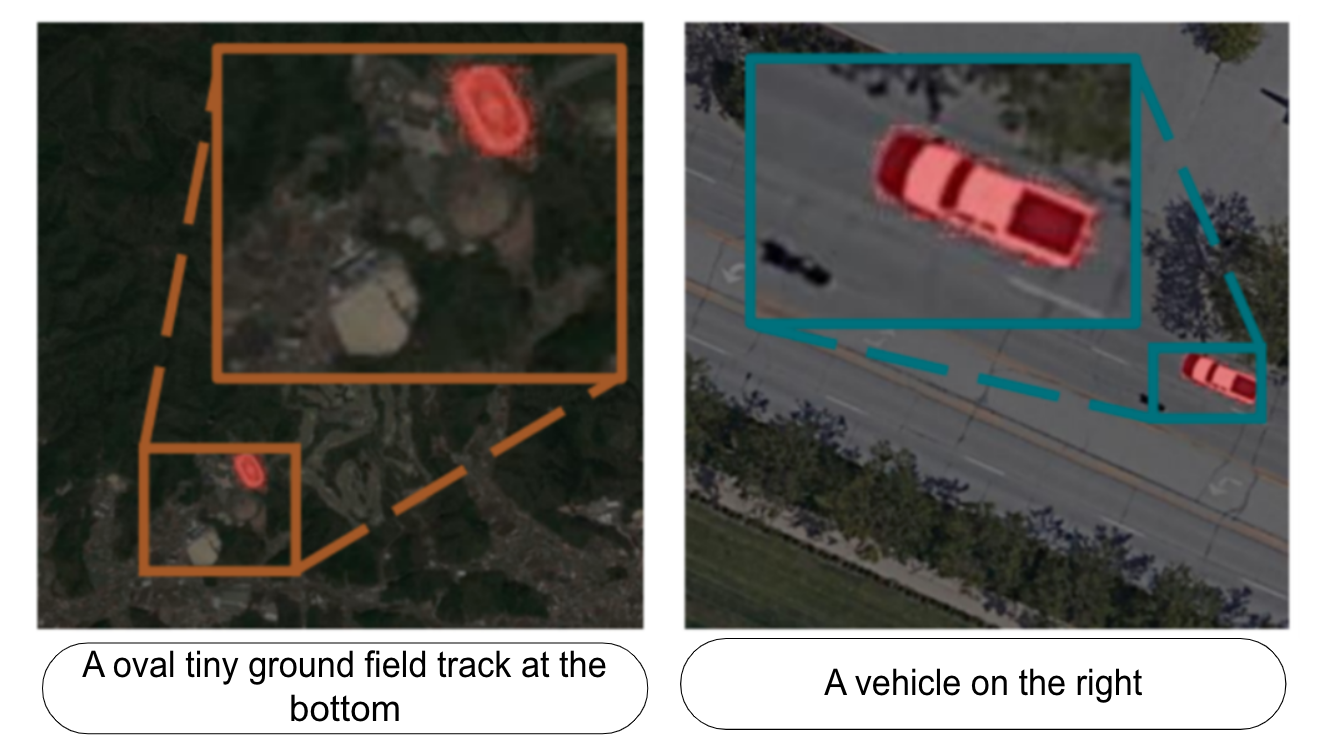
\includegraphics[width=0.45\textwidth]{Images/rrsisd.png}\label{fig:rrsisd}}
\caption{Examples from aerial referring segmentation datasets showing diverse referring expressions with corresponding images and ground truth masks.}
\label{fig:aerial_datasets}
\end{figure}

[Reference to NWPU-Refer dataset] % \cite{placeholder_nwpu}

[diagram for NWPU-Refer dataset example samples]

\begin{table}[htbp]
\centering
\caption{Aerial Referring Segmentation (RRSIS) Dataset Comparison}
\label{tab:rrsis_comparison}
\begin{tabular}{@{}llll@{}}
\toprule
\textbf{Feature} & \textbf{RefSegRS} & \textbf{RRSIS-D} & \textbf{NWPU-Refer} \\
\midrule
Size & 4,420 triplets & 17,402 triplets & 49,745 triplets \\
Source & SkyScapes & RSVGD & Multi-source global \\
Annotation & Manual & Semi-auto (SAM) & Manual \\
Resolution & Limited & 800×800 fixed & 1024-2048px \\
Focus & RRSIS & RRSIS & RRSIS \\
Categories & - & 20 & 32 \\
Attributes & 3 & 7 & 6 dimensions \\
\bottomrule
\end{tabular}
\end{table}

\begin{table}[htbp]
\centering
\caption{Source Aerial Dataset Comparison}
\label{tab:source_comparison}
\begin{tabular}{@{}lll@{}}
\toprule
\textbf{Feature} & \textbf{iSAID} & \textbf{LoveDA} \\
\midrule
Size & 655,451 instances & 5,987 images \\
Source & DOTA (re-ann.) & Spaceborne (0.3m) \\
Annotation & Professional & Manual \\
Resolution & High res. & 1024×1024px \\
Focus & Instance Seg. & Land-cover Seg. + UDA \\
Categories & 15 & 7 \\
Attributes & - & Domain labels \\
\bottomrule
\end{tabular}
\end{table}

\begin{table}[htbp]
\centering
\caption{RRSIS Dataset Split Statistics}
\label{tab:rrsis_splits}
\begin{tabular}{@{}llllll@{}}
\toprule
\textbf{Dataset} & \textbf{Total} & \textbf{Training} & \textbf{Validation} & \textbf{Test} & \textbf{Unit} \\
\midrule
RefSegRS & 4,420 & 2,172 (49.1\%) & 431 (9.8\%) & 1,817 (41.1\%) & expressions \\
RRSIS-D & 17,402 & 8,701 (50.0\%) & 3,480 (20.0\%) & 5,221 (30.0\%) & triplets \\
NWPU-Refer & 49,745 & 34,821 (70.0\%) & 4,974 (10.0\%) & 9,950 (20.0\%) & triplets \\
\bottomrule
\end{tabular}
\end{table}

\begin{table}[htbp]
\centering
\caption{Source Dataset Split Statistics}
\label{tab:source_splits}
\begin{tabular}{@{}llllll@{}}
\toprule
\textbf{Dataset} & \textbf{Total} & \textbf{Training} & \textbf{Validation} & \textbf{Test} & \textbf{Unit} \\
\midrule
iSAID & 2,806 & 1,403 (50.0\%) & 468 (16.7\%) & 935 (33.3\%) & images \\
LoveDA & 5,987 & 2,522 (42.1\%) & 1,669 (27.9\%) & 1,796 (30.0\%) & images \\
\bottomrule
\end{tabular}
\end{table}

% #############################################################################
\section{Segmentation Models for Aerial Images}

This section examines the landscape of segmentation models specifically designed for or applicable to aerial imagery analysis, encompassing both semantic segmentation approaches and referring segmentation techniques.

\subsection{Semantic Segmentation Models}

Foundational vision models provide the backbone architectures for aerial image segmentation tasks through powerful feature extraction and mask generation capabilities.

Vision-language models such as CLIP establish crucial connections between visual and textual modalities through contrastive learning, enabling zero-shot classification capabilities that transfer effectively to aerial imagery domains. The learned joint embedding spaces capture semantic relationships that prove valuable for understanding aerial scene content and object categories.

SigLIP represents an advancement in vision-language training methodologies, improving upon CLIP's contrastive approach through more efficient training objectives and enhanced representation learning. These improvements translate to better performance on downstream aerial image understanding tasks where precise visual-textual alignment is critical.

The Segment Anything Model (SAM) provides a foundational approach to semantic segmentation through its prompt-based architecture, as illustrated in Figure~\ref{fig:sam_architecture}. SAM's design incorporates an image encoder that processes input imagery into rich feature representations, a prompt encoder that handles various input modalities including points, boxes, and text, and a mask decoder that generates precise segmentation boundaries. This architecture demonstrates remarkable generalization capabilities across diverse image domains, including aerial imagery, where its ability to process multiple prompt types enables flexible segmentation workflows that can adapt to different user requirements and annotation strategies.

\begin{figure}[htbp]
\centering
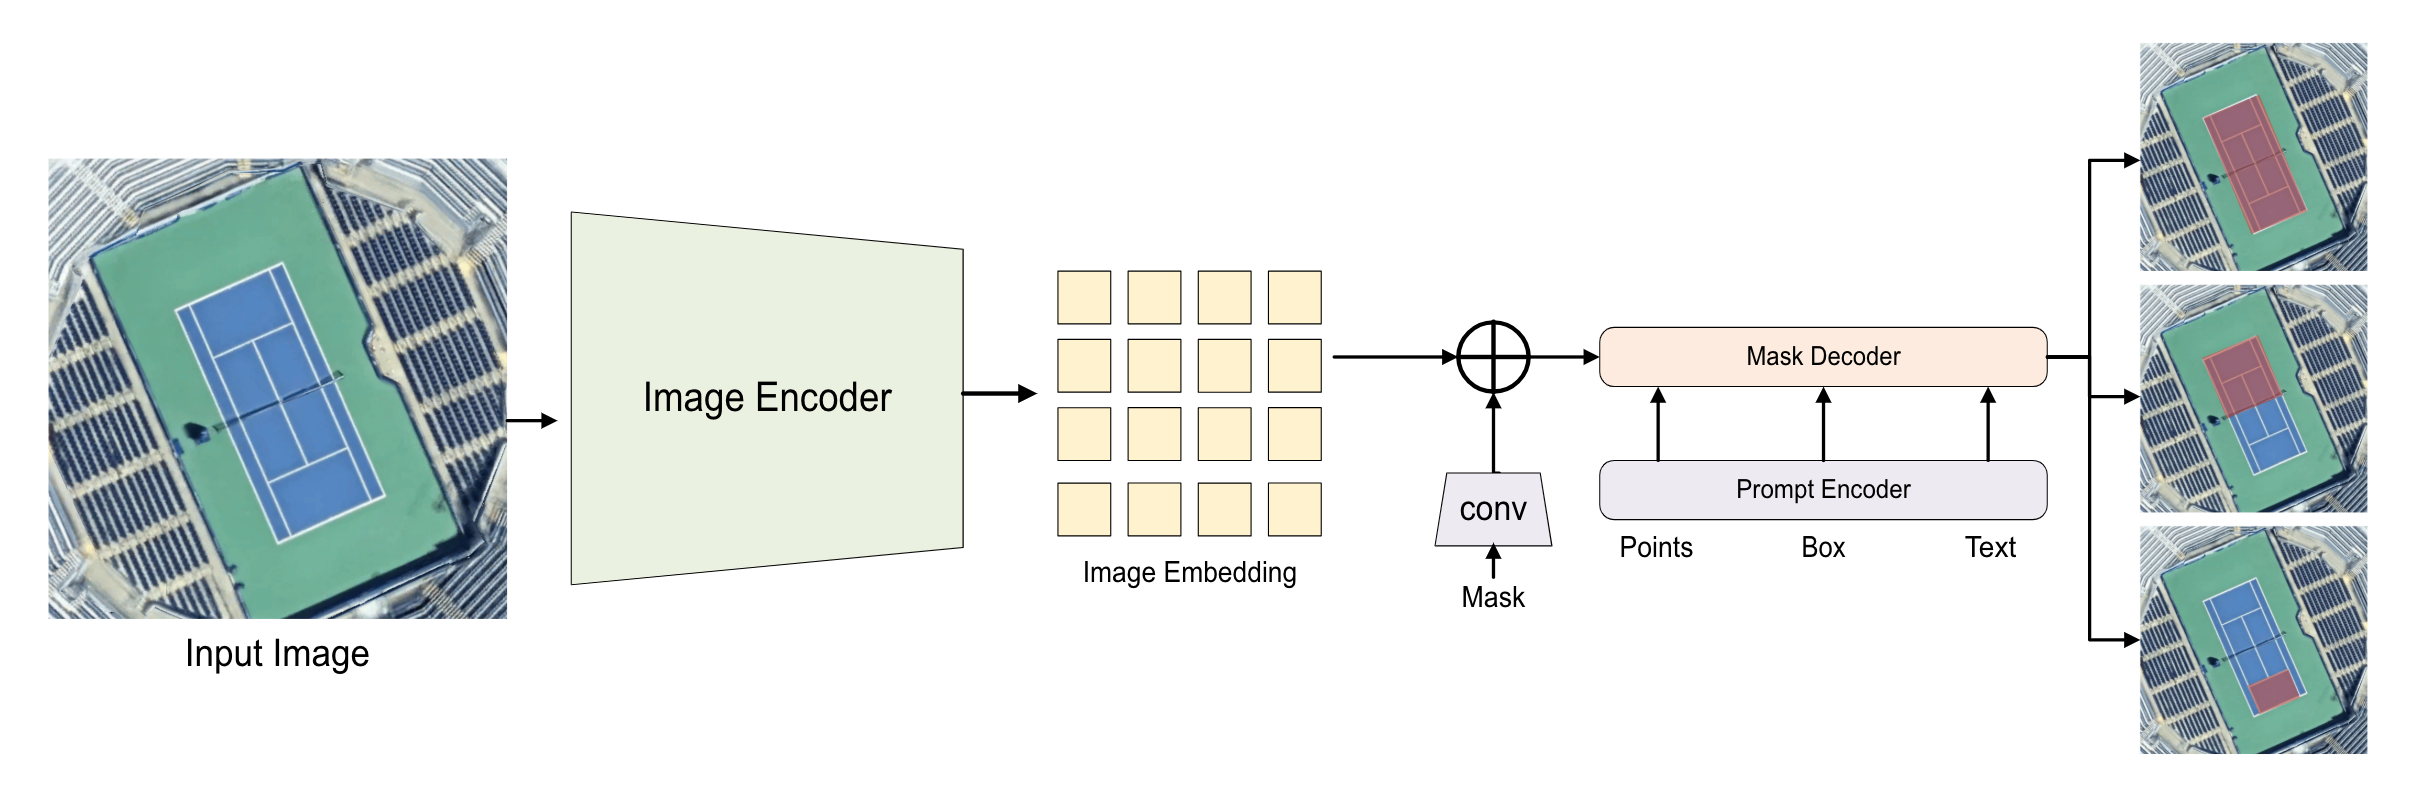
\includegraphics[width=1.0\textwidth]{Images/sam.png}
\caption{Segment Anything Model (SAM) architecture showing the image encoder, prompt encoder, and mask decoder components. The model processes various prompt types including points, boxes, and text to generate precise segmentation masks.}
\label{fig:sam_architecture}
\end{figure}

\subsection{Referring Segmentation Models}

Advanced referring segmentation approaches combine semantic understanding with natural language comprehension to enable text-guided segmentation in aerial imagery contexts.

Previous approaches to language-guided segmentation have established important foundations for referring segmentation in natural images. LAVT introduces attention-based fusion mechanisms that align textual and visual features for precise object localization and segmentation. RMSIN advances multi-scale integration strategies that capture objects at different scales and resolutions. FIANet demonstrates the effectiveness of feature interaction architectures that enable sophisticated text-visual reasoning for segmentation tasks.

RSRefSeg represents a specialized approach designed specifically for aerial referring segmentation, as shown in Figure~\ref{fig:rsrefseg_architecture}. The architecture integrates SigLIP2 vision-language encoders with SAM mask decoders through custom prompter networks that process text-guided segmentation requests. The dual-pathway design processes both local token-level and global sentence-level text-visual interactions, generating sparse and dense prompts that enable precise aerial image segmentation guided by natural language descriptions. This architecture addresses the unique challenges of aerial imagery analysis, including varied object scales, complex spatial relationships, and domain-specific terminology requirements.

\begin{figure}[H]
\centering
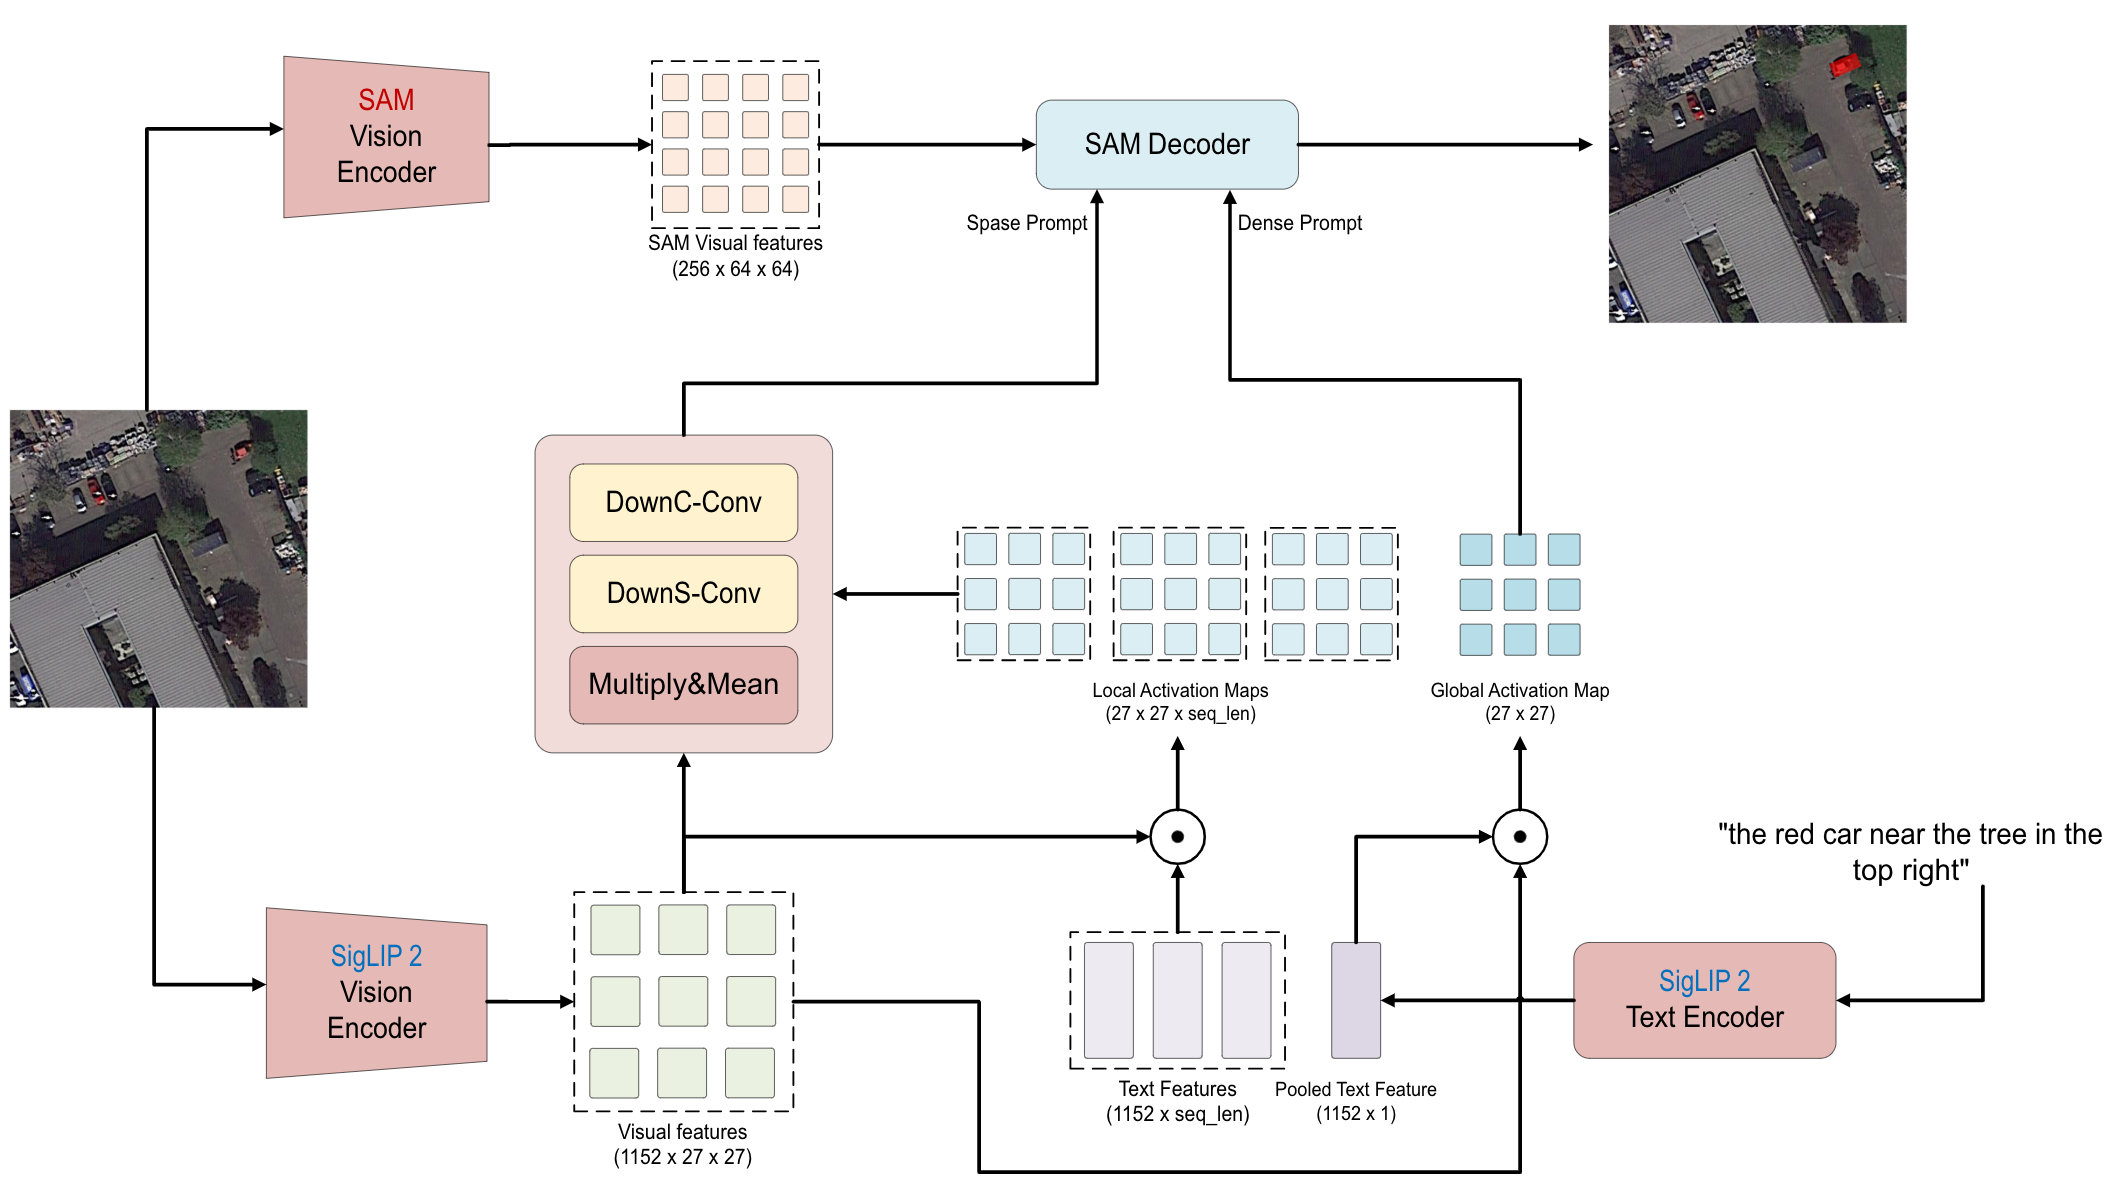
\includegraphics[width=\textwidth]{./Images/clipsam.png}
\caption{RSRefSeg architecture overview showing the integration of SigLIP2 vision-language encoder with SAM mask decoder through custom prompter networks for text-guided segmentation. The dual-pathway design processes both local (token-level) and global (sentence-level) text-visual interactions to generate sparse and dense prompts for precise aerial image segmentation.}
\label{fig:rsrefseg_architecture}
\end{figure}

% #############################################################################
\section{Overview}

[Synthesis of all related work - gaps identified and how this work addresses them] % \cite{placeholder_synthesis}
% If Printing on DOUBLE SIDED pages, the second page should be white.
% Otherwise, comment the following command:
\cleardoublepage
%
%Chapter 4
% #############################################################################
% This is Chapter 4
% !TEX root = ../main.tex
% #############################################################################
% Change the Name of the Chapter i the following line
\fancychapter{Dataset Construction}
\cleardoublepage
% The following line allows to ref this chapter
\label{chap:implement}

This chapter presents the systematic approach for constructing the AerialD dataset for open-vocabulary aerial image segmentation. Our methodology transforms existing aerial datasets into a comprehensive referring segmentation resource through automated rule-based generation and LLM enhancement.

% #############################################################################
\section{Source Datasets}

\noindent The AerialD dataset is constructed from two primary sources of aerial imagery with fundamentally different annotation paradigms, as illustrated in Table~\ref{tab:dataset_sources}. The iSAID dataset is an instance segmentation dataset providing high-resolution aerial images with precise boundaries for individual object instances across fifteen categories including ships, vehicles, planes, buildings, and infrastructure elements such as harbors and bridges. In contrast, the LoveDA dataset is a semantic segmentation dataset that captures land cover and land use patterns, providing pixel-level classification into categories such as buildings, water bodies, agricultural areas, forests, and barren land. These two datasets ensure comprehensive coverage of both discrete objects and continuous landscape features commonly encountered in aerial imagery analysis.


% Dataset sources table with images
\begin{table}[H]
\centering
\caption{Source Dataset Characteristics}
\label{tab:dataset_sources}
\begin{tabular}{@{}p{4cm}p{8cm}@{}}
\toprule
\multicolumn{2}{c}{\textbf{iSAID Dataset}} \\
\midrule
\raisebox{-0.5\height}{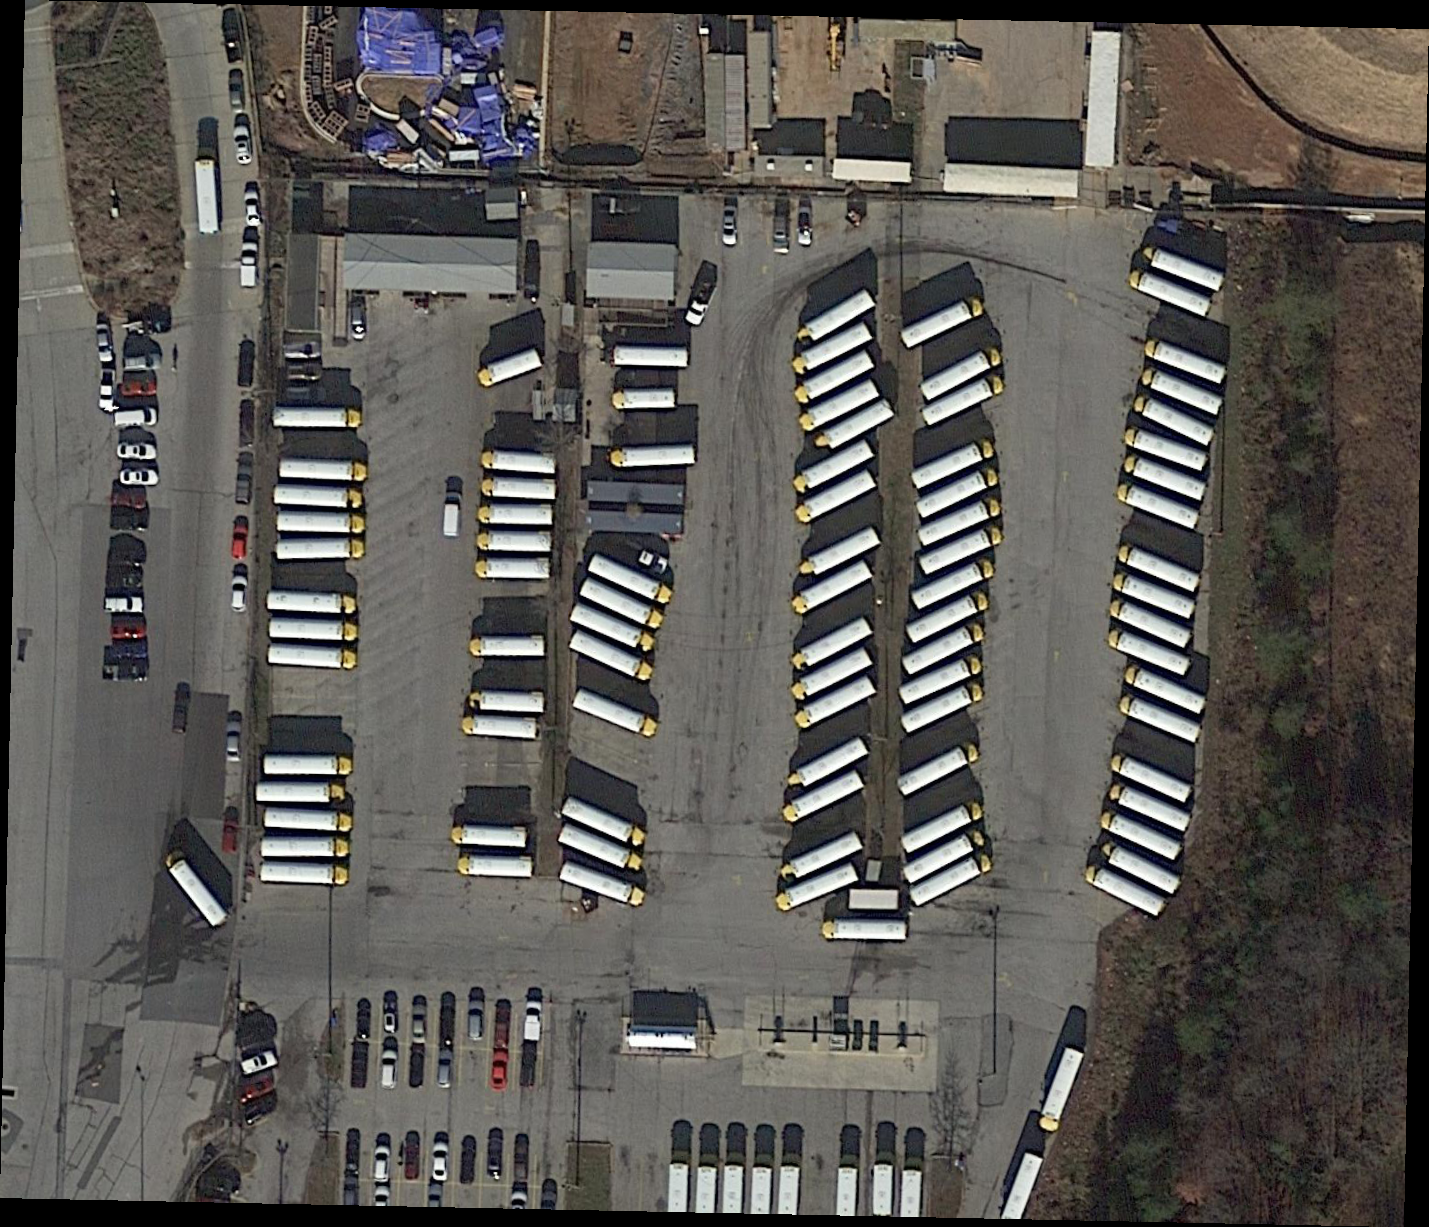
\includegraphics[width=3.5cm, height=3.5cm]{./Images/isaid.png}} & 
\hspace{-0.5cm}\parbox[c]{8cm}{\fontsize{10pt}{12pt}\selectfont Contains \textbf{2,806} high resolution images at varying widths of 800 to 13,000 pixels, spatial resolution of \textbf{0.1m to 4.5m}, with \textbf{655,451} instances across \textbf{15} object classes including \textbf{ships}, \textbf{large vehicles}, \textbf{small vehicles}, \textbf{planes}, etc.} \\[0.5cm]
\midrule
\multicolumn{2}{c}{\textbf{LoveDA Dataset}} \\
\midrule
\raisebox{-0.5\height}{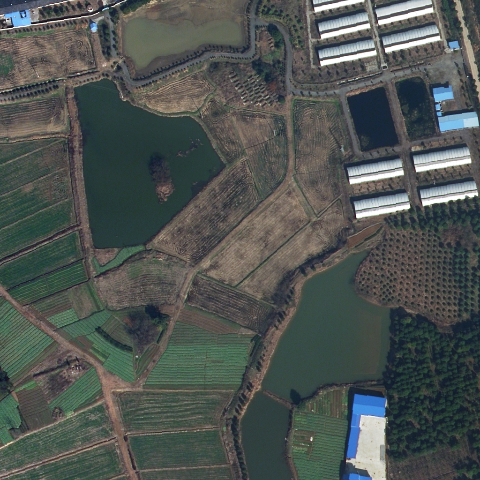
\includegraphics[width=3.5cm, height=3.5cm]{./Images/loveda_dataset.png}} & 
\hspace{-0.5cm}\parbox[c]{8cm}{\fontsize{10pt}{12pt}\selectfont Contains \textbf{5,987} images at 1024 pixel width, spatial resolution of \textbf{0.3m}, across \textbf{6} land cover classes: \textbf{building}, \textbf{road}, \textbf{water}, \textbf{barren}, \textbf{forest}, and \textbf{agriculture}.} \\[0.5cm]
\bottomrule
\end{tabular}
\end{table}

% #############################################################################
% #############################################################################
\section{Rule-Based Expression Generation}

The rule-based expression generation pipeline systematically transforms semantic segmentation and instance segmentation datasets into referring expression datasets through a sequential five-step process that analyzes spatial, visual, and relational properties of objects and groups within aerial imagery. This comprehensive approach begins with patch extraction from source datasets and culminates in linguistically diverse and contextually accurate referring expressions.

The process initiates with iSAID patch extraction, where instance annotations are loaded from COCO-format JSON files containing 655,451 instances across 15 object categories. The system extracts 480$\times$480 patches using a sliding window approach with 20\% overlap, processing both training and validation splits through multiprocessing for computational efficiency. The sliding window approach creates the risk that objects may be partially cut off at patch boundaries, where a cutoff object is defined as an instance whose segmentation polygon extends beyond the extracted patch area. Critical to maintaining annotation quality, the extraction process handles cutoff objects by calculating intersection ratios, marking instances where less than 50\% remains within patch boundaries and fewer than 500 pixels are visible as potentially unreliable. Polygon segmentations are converted to run-length encoding (RLE) format for storage efficiency, while we extract essential metadata from JSON annotations including bounding boxes, areas, and segmentation data. The system filters out patches with excessive black pixels exceeding a 50\% threshold, ensuring visual content quality throughout the dataset.

LoveDA patch processing follows a distinct approach tailored to semantic segmentation data from 1024$\times$1024 images across urban and rural domains. The system resizes the entire image to 480$\times$480 dimensions to maintain consistency with iSAID patches. For ``building'' and ``water'' categories, the system converts semantic segmentation masks into individual instance segmentation masks through connected components analysis. This selective conversion makes sense because LoveDA's land cover classification design means that buildings and water bodies naturally occur as discrete, spatially bounded entities with clear geometric boundaries, making them suitable for instance segmentation. In contrast, classes such as agriculture, forest, and barren land represent diffuse land cover types that extend across large continuous regions without natural instance boundaries, making individual instance extraction neither meaningful nor reliable for these categories.

For LoveDA building and water categories, individual instances are extracted using connected components analysis, which identifies spatially connected regions within each semantic class by examining pixel connectivity patterns. The algorithm traverses the binary mask where pixels are considered connected if they are adjacent horizontally, vertically, or diagonally, meaning each pixel can connect to any of its eight neighboring pixels in the surrounding 3$\times$3 grid, effectively grouping contiguous pixels belonging to the same semantic class into distinct labeled regions. Connected components below minimum area thresholds of 50 pixels for buildings and 100 pixels for water are filtered out to eliminate spurious detections. This dual-layer processing creates both individual building and water instances for referring expression generation, while simultaneously preserving the complete semantic segmentation masks containing all pixels of each class. Agricultural areas, forests, and barren land are exclusively treated as unified semantic classes, with single masks encompassing all pixels of each category and pre-written expressions such as ``all buildings in the image'' generated for these class-level groups, while multiprocessing handles both urban and rural domains efficiently.

Having established 480$\times$480 patches with annotated object instances and masks from both iSAID and LoveDA processing, the pipeline proceeds to the core rule addition and analysis phase, which transforms these basic annotations into rich spatial and visual descriptions through systematic feature extraction. Each 480$\times$480 patch undergoes partitioning into a three-by-three grid establishing nine distinct spatial regions, as illustrated in Figure \ref{fig:rule_example}. The grid divides the image into equal thirds both horizontally and vertically, creating regions such as ``top left'', ``center'', and ``bottom right''. However, objects positioned near grid boundaries present a challenge, as instances separated by just a few pixels between adjacent regions could create ambiguity in referring expressions and confuse models about which specific object is being referenced. To address this boundary ambiguity, the system implements borderline detection using a boundary threshold of 10\% of the image dimensions. When an object's centroid falls within this boundary zone (48 pixels from any grid line in a 480$\times$480 image), the system generates multiple valid position labels for that instance. For example, an object near the boundary between ``top center'' and ``center center'' regions receives both position labels as valid alternatives. This dual-labeling strategy ensures robust expression generation, as conflicting expressions referencing the same borderline object will be filtered out in subsequent deduplication steps, while maintaining coverage for legitimate spatial references.

To provide comprehensive visual features for referring expressions, the system performs color classification for each individual object instance. The classification process operates on HSV color space pixels extracted from segmentation masks, first distinguishing between achromatic and chromatic colors through saturation analysis. Objects are classified as achromatic when their saturation levels fall below 25\%, further subdivided into light and dark categories using a brightness threshold of 54\%. For chromatic instances, the system identifies specific hue ranges across eight distinct colors: red, orange, yellow, green, cyan, blue, purple, and magenta, with each hue occupying predetermined angular ranges within the HSV color wheel. The system requires 70\% dominance thresholds for both achromatic and chromatic classifications to ensure reliable color assignment. Importantly, the system does not assign colors to every instance, particularly in cases where multiple hues are present within a single object or when the color distribution is ambiguous, as assigning incorrect color labels could create misleading referring expressions.

In order to provide additional spatial context beyond grid positioning, the system introduces extreme position detection to identify instances that occupy boundary locations within their respective object categories. This analysis proves particularly valuable for scenes containing multiple objects of the same type, where conventional grid-based positioning may be insufficient for unique identification. The system determines topmost, bottommost, leftmost, and rightmost instances within each category by first sorting objects by their centroid coordinates, then applying a separation threshold to ensure meaningful distinctions. Specifically, the system uses a margin ratio of 5\% of the image dimensions (24 pixels in a 480$\times$480 image) to verify that the most extreme object is sufficiently separated from the second-most extreme object before assigning the extreme position label. For example, for topmost detection, the system compares the y-coordinates of the two highest objects and only assigns the ``topmost'' label if their vertical separation exceeds the margin threshold, enabling reliable expressions such as ``the leftmost ship'' or ``the topmost building'' when multiple instances of the same class are present.

To enable complex referring expressions that describe objects in terms of their proximity to other instances, the system implements spatial relationship calculation. This addresses cases where objects need to be localized relative to nearby instances within the scene, particularly when absolute grid positions alone cannot provide sufficient discriminative information. The system employs an angle-based directional system calculating angular relationships between object centroids to determine relative positioning using eight distinct directions: to the left of, to the bottom left of, below, to the bottom right of, to the right of, to the top right of, above, and to the top left of. However, establishing relationships between all possible object pairs would create spurious connections between distant objects that provide no meaningful spatial context for referring expressions, potentially leading to confusing references like "the ship to the left of a building" when the building is at the opposite edge of the image. To address this problem, the system limits relationships to nearby instances using dynamic distance thresholds rather than fixed distances. A fixed threshold would incorrectly discard meaningful relationships involving large objects, such as when a vehicle appears to the left of a large roundabout whose centroid lies at its geometric center - the fixed distance from the vehicle to the roundabout's centroid might exceed the threshold despite their obvious spatial relationship. The dynamic threshold starts with a base maximum distance of 150 pixels, then adds half the average size of both source and target objects to account for object scale. For example, when relating two large buildings with average dimensions of 60 pixels, the maximum relationship distance becomes 210 pixels (150 + 30 + 30), ensuring that larger objects can establish relationships across greater distances than smaller objects while preventing meaningless long-distance connections. When objects fall near angular boundaries between directional zones, the system handles these borderline cases by recording multiple directional possibilities, similar to the absolute grid positioning borderline detection, ensuring comprehensive coverage of spatial interpretations and preventing arbitrary assignment decisions.

To handle scenarios where multiple instances of the same object category appear within patches, the system introduces group formation to enable collective referring expressions and reduce annotation redundancy. This addresses the challenge of creating natural language expressions when numerous similar objects are present, where individual instance references would become unwieldy or ambiguous. The system utilizes DBSCAN clustering with carefully tuned parameters: epsilon distance of 40 pixels, minimum cluster size of 2 objects, and maximum cluster size of 8 objects, operating separately within each object category to maintain semantic coherence. Class-level groups are automatically generated for categories containing multiple instances, creating expressions such as ``all ships in the image'' when numerous instances of the same type are present. Additionally, the system creates special pair groups that combine small and large vehicles when both vehicle types coexist within patches, enabling more natural referring expressions that reference vehicle collections rather than individual instances.

\begin{figure}[H]
\centering
\begin{minipage}{0.5\textwidth}
\centering
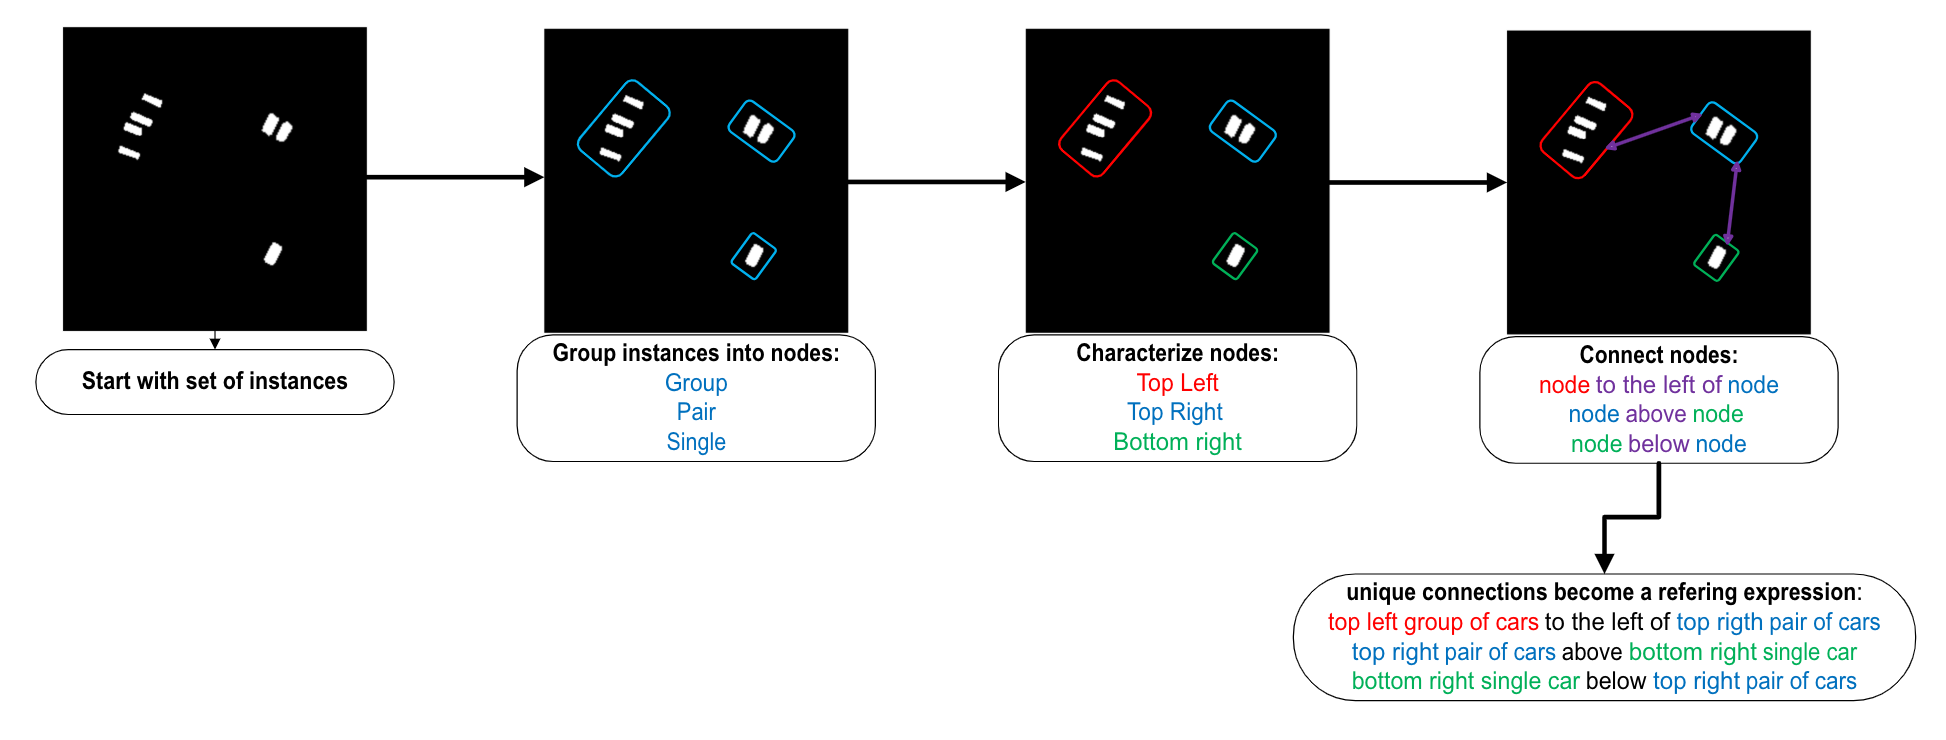
\includegraphics[width=0.7\textwidth]{./Images/rule_based_generation.png}
\end{minipage}%
\begin{minipage}{0.5\textwidth}
\centering
\hspace{-1cm}
\raisebox{-0.3\height}{%
\resizebox{\textwidth}{!}{%
\footnotesize
\begin{tabular}{@{}ll@{}}
\toprule
\textbf{Rule Type} & \textbf{Example Instance} \\
\midrule
Category & "plane" \\
Grid Position & "in the top right" \\
Extreme Position & None \\
Color Classification & "light" \\
Directional Relations & "to the bottom right of a plane" \\
& "to the top right of a plane" \\
\midrule
\multicolumn{2}{l}{\textbf{Final Expressions}} \\
\multicolumn{2}{l}{"the plane in the top right"} \\
\multicolumn{2}{l}{"the light plane in the top right"} \\
\multicolumn{2}{l}{"the plane in the top right to the bottom right of a plane"} \\
\multicolumn{2}{l}{"the light plane in the top right to the bottom right of a plane"} \\
\multicolumn{2}{l}{"the plane in the top right to the top right of a plane"} \\
\multicolumn{2}{l}{"the light plane in the top right to the top right of a plane"} \\
\bottomrule
\end{tabular}%
}%
}
\end{minipage}
\caption{Example of rule generation for a single instance. The highlighted plane in the top right section demonstrates how the system assigns spatial, visual, and relational rules that will later be combined into referring expressions.}
\label{fig:rule_example}
\end{figure}

The expression generation engine operates through combinatorial synthesis of extracted attributes, creating comprehensive linguistic descriptions by systematically enumerating all valid combinations of category labels, grid positions, spatial relationships, extreme positions, size characteristics, and color properties. The system implements seventeen distinct expression templates ranging from simple category-only descriptions like ``the ship'' to complex multi-attribute formulations such as ``the dark largest ship in the top right that is above a building''. Color expression filtering removes chromatic color references from buildings and water to maintain semantic appropriateness, while borderline cases generate multiple expression variants to ensure comprehensive coverage of spatial and relational interpretations. Group expressions handle multi-instance clusters with appropriate size quantifiers and plural forms, while dummy expression marking tags potentially unreliable expressions originating from cutoff objects or ambiguous relationships for subsequent filtering.

Uniqueness filtering ensures expression quality and eliminates ambiguity through systematic standardization and deduplication processes. The system converts class names from technical formats to natural language equivalents, transforming ``Large\_Vehicle'' to ``large vehicle'' and applying appropriate pluralization logic based on group sizes and context. Expression standardization normalizes linguistic variations while preserving semantic meaning, followed by duplicate detection that identifies and removes expressions appearing multiple times across the dataset. The strict deduplication policy eliminates all occurrences of non-unique phrases, preventing ambiguous references that would compromise the referring expression task. Dummy expressions from cutoff objects are removed after uniqueness checking to maintain only high-confidence annotations, while objects and groups lacking valid expressions are eliminated entirely from the dataset.

% Expression uniqueness filter example
\begin{figure}[H]
\centering
\begin{minipage}{0.5\textwidth}
\centering
\includegraphics[width=0.7\textwidth]{./Images/filter_unique.png}
\end{minipage}%
\begin{minipage}{0.5\textwidth}
\centering
\hspace{-1cm}
\raisebox{-0.3\height}{%
\resizebox{\textwidth}{!}{%
\footnotesize
\begin{tabular}{@{}ll@{}}
\toprule
\textbf{Expression} & \textbf{Status} \\
\midrule
\multicolumn{2}{l}{\textbf{Object 1 (Light Vehicle)}} \\
\midrule
"the small vehicle in the top right" & \textcolor{red}{Filtered} \\
"the topmost small vehicle" & \textcolor{green!70!black}{Kept} \\
"the light small vehicle in the top right" & \textcolor{green!70!black}{Kept} \\
"the light topmost small vehicle" & \textcolor{green!70!black}{Kept} \\
"the small vehicle in the top right above a small vehicle" & \textcolor{green!70!black}{Kept} \\
\midrule
\multicolumn{2}{l}{\textbf{Object 2 (Dark Vehicle)}} \\
\midrule
"the small vehicle in the top right" & \textcolor{red}{Filtered} \\
"the dark small vehicle in the top right" & \textcolor{green!70!black}{Kept} \\
"the small vehicle in the top right below a small vehicle" & \textcolor{green!70!black}{Kept} \\
\bottomrule
\end{tabular}%
}%
}
\end{minipage}
\caption{Example of expression uniqueness filtering showing how ambiguous expressions are removed when multiple objects occupy similar spatial positions. The blue and red boxes highlight two small vehicles in the top right corner that would create conflicting references.}
\label{fig:uniqueness_filter}
\end{figure}



% #############################################################################
\section{LLM Expression Generation}

Beyond rule-based expression generation, we further enhance the dataset through multimodal large language model fine-tuning. We leverage the generalization capabilities of open-source multimodal LLMs, which possess both advanced language understanding and vision processing capabilities, to create more natural and diverse referring expressions. Through fine-tuning a multimodal LLM specifically on the task of expression enhancement, we apply this enhanced model to the full extent of our rule-based dataset, more than doubling the number of expressions from the original rule-based generation and significantly increasing the linguistic diversity and naturalness of the referring expressions.

% LLM enhancement example figure
\begin{figure}[H]
\centering
\begin{minipage}{0.5\textwidth}
\centering
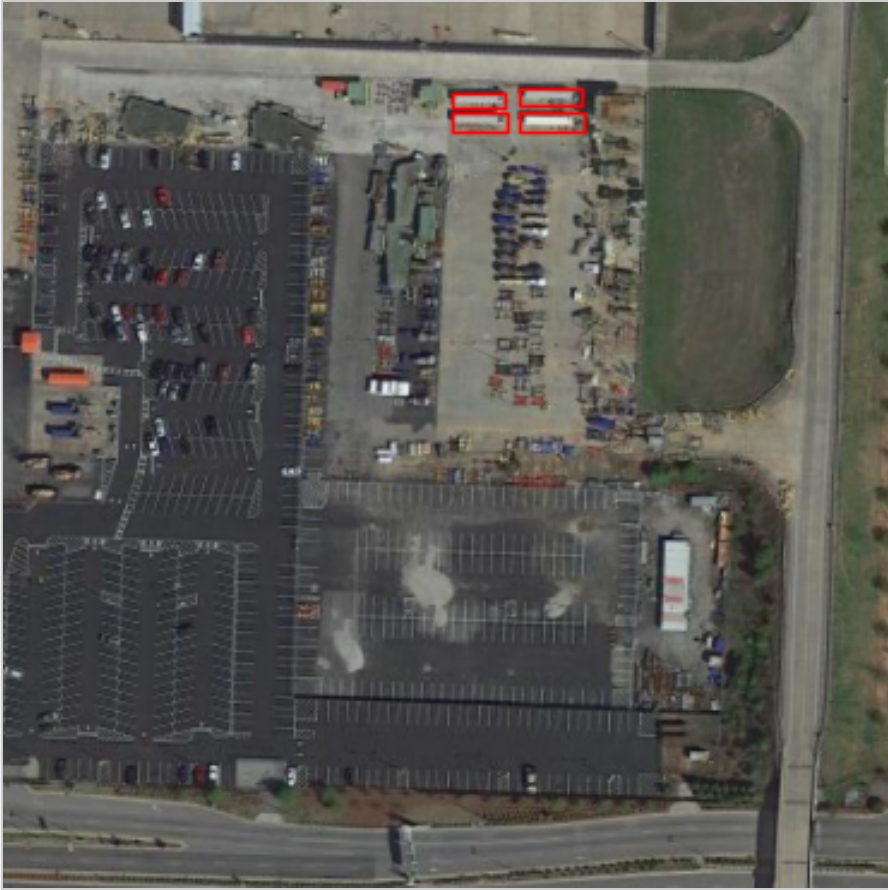
\includegraphics[width=0.7\textwidth]{./Images/example_group.png}
\end{minipage}%
\begin{minipage}{0.5\textwidth}
\centering
\hspace{-1cm}
\raisebox{-0.3\height}{%
\footnotesize
\begin{tabular}{@{}p{2cm}p{5cm}@{}}
\toprule
\textbf{Expression Type} & \textbf{Example} \\
\midrule
Original & the group of 4 large vehicles in the top center \\
\midrule
Enhanced & the cluster of four big vehicles near the upper middle \\
\midrule
Unique & the four large vehicles lined up side by side just below the pale paved strip at the very top middle \\
\midrule
Unique & the set of four big vehicles parked in a single row in the upper center beside the grassy area to the right \\
\bottomrule
\end{tabular}%
}
\end{minipage}
\caption{Example of LLM enhancement process showing original aerial image with group of four large vehicles (left) and corresponding expression enhancements (right).}
\label{fig:llm_enhancement_example}
\end{figure}

% #############################################################################
\section{LLM Distillation}

Knowledge distillation enables scalable enhancement of the full dataset by transferring capabilities from large proprietary models to smaller, locally deployable models.

\begin{figure}[H]
\centering
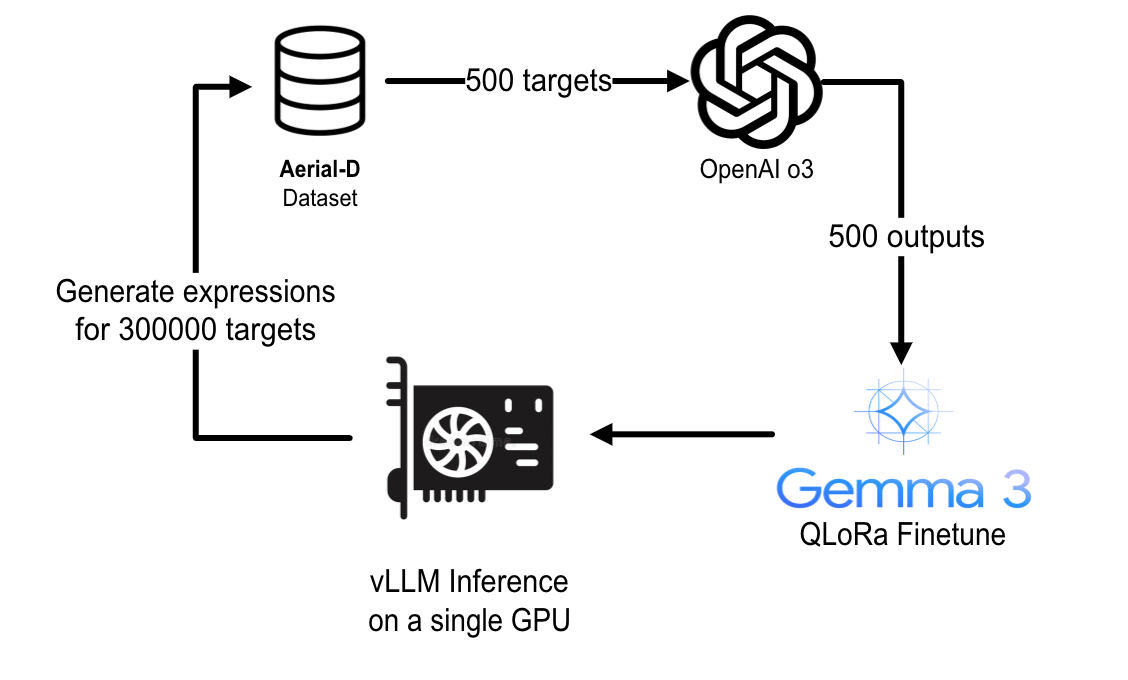
\includegraphics[width=0.8\textwidth]{./Images/distillation.png}
\caption{Knowledge distillation pipeline for scalable LLM enhancement. A small sample of 500 expressions is processed through OpenAI's O3 model to generate high-quality training targets, which are then used to fine-tune Gemma3 12B via QLora. The fine-tuned model enables cost-effective local inference to enhance the full dataset of 300,000 expressions using vLLM on a single GPU.}
\label{fig:llm_distillation}
\end{figure}


% #############################################################################
\section{Final Dataset Statistics}

The completed AerialD dataset represents a comprehensive resource for aerial referring expression segmentation, combining rule-based generation with LLM enhancement to create diverse and natural language descriptions.

% Dataset examples figure
\begin{figure}[H]
\centering
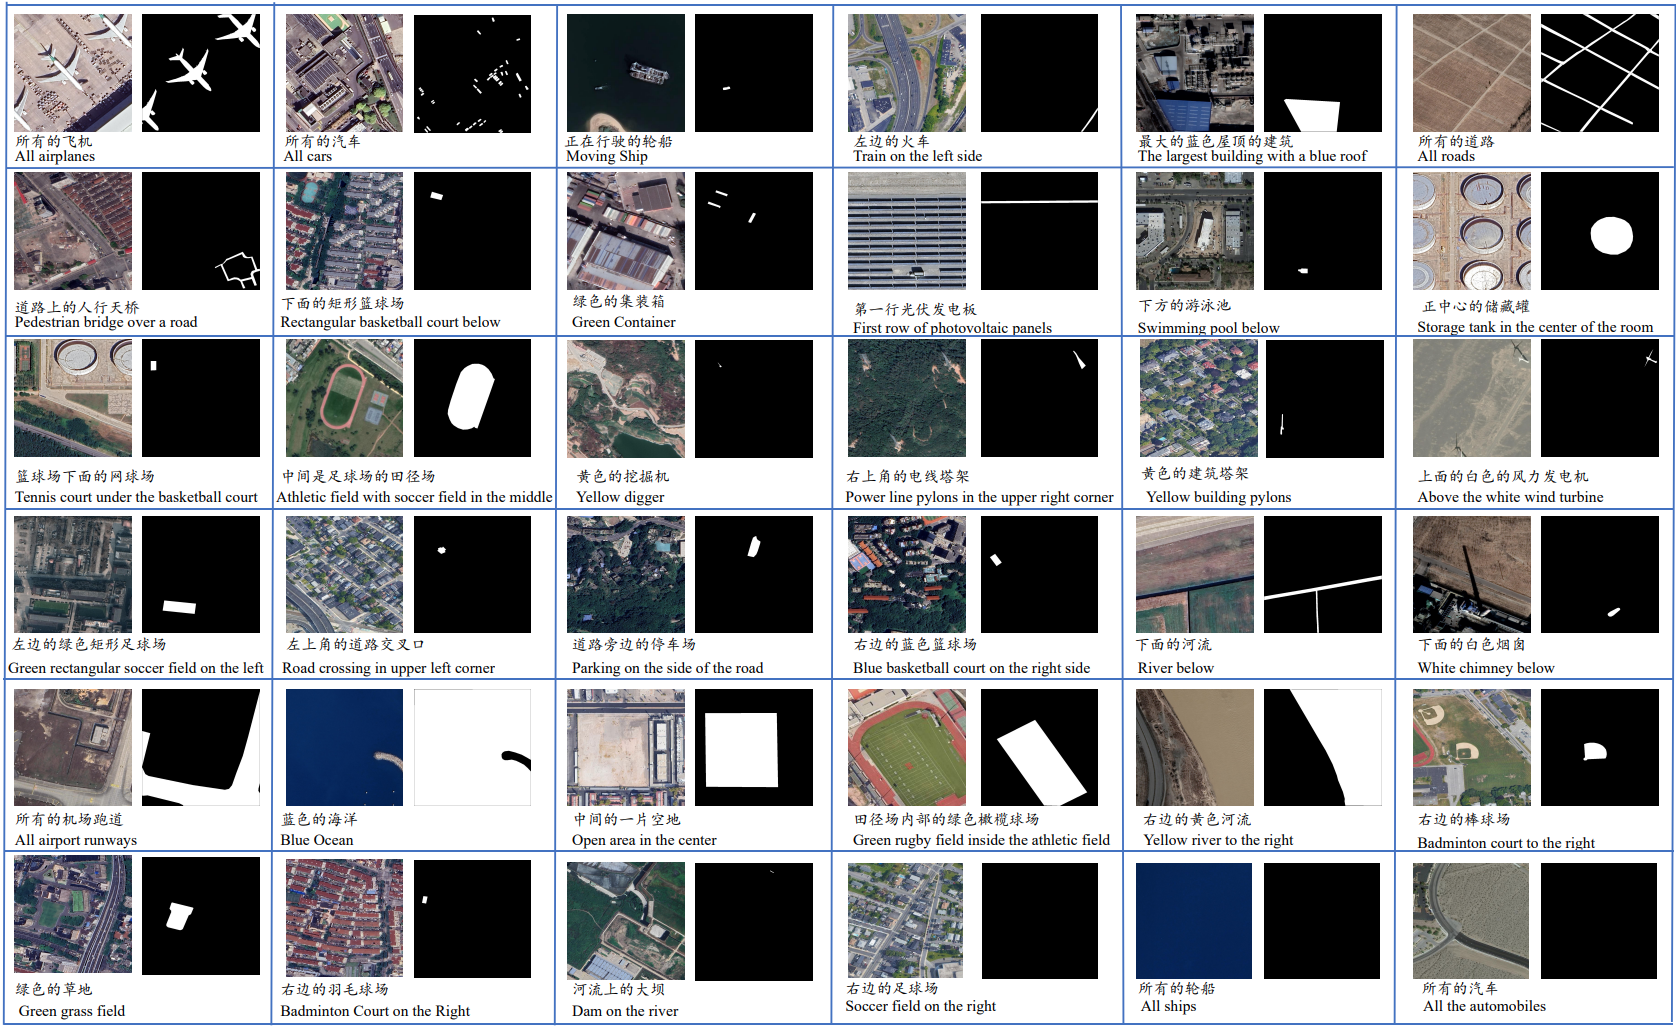
\includegraphics[width=\textwidth]{./Images/dataset.png}
\caption{Representative examples from AerialD dataset showing diverse referring expressions with corresponding aerial images and ground truth masks.}
\label{fig:dataset_examples}
\end{figure}

% Dataset statistics table
\begin{table}[H]
\centering
\caption{Dataset Statistics Summary}
\label{tab:dataset_stats}
\begin{tabular}{@{}lrrr@{}}
\toprule
\textbf{Metric} & \textbf{Train} & \textbf{Val} & \textbf{Total} \\
\midrule
Total Patches & 27,480 & 9,808 & 37,288 \\
Individual Objects with Expressions & 94,179 & 34,536 & 128,715 \\
Individual Expressions & 646,686 & 242,668 & 889,354 \\
Groups with Expressions & 96,832 & 34,162 & 130,994 \\
Group Expressions & 471,108 & 162,061 & 633,169 \\
Total Samples & 191,011 & 68,698 & 259,709 \\
Avg. Expressions per Individual Object & 6.87 & 7.03 & 6.91 \\
Avg. Expressions per Group & 4.87 & 4.74 & 4.83 \\
\bottomrule
\end{tabular}
\end{table}

% Category distribution table
\begin{table}[H]
\centering
\caption{Object Category Distribution by Instance Type and Source Dataset}
\label{tab:category_dist}
\resizebox{\textwidth}{!}{%
\begin{tabular}{@{}lrrrrr@{}}
\toprule
\textbf{Category} & \textbf{Individual Instances} & \textbf{Groups} & \textbf{Instance Expressions} & \textbf{Group Expressions} & \textbf{Source Dataset} \\
\midrule
Ship & 11,461 & 10,402 & 79,251 & 49,272 & iSAID \\
Large Vehicle & 17,425 & 18,496 & 121,593 & 95,356 & iSAID \\
Small Vehicle & 41,353 & 53,682 & 262,831 & 282,848 & iSAID \\
Storage Tank & 2,985 & 3,451 & 19,537 & 16,071 & iSAID \\
Harbor & 9,164 & 6,290 & 72,248 & 28,613 & iSAID \\
Swimming Pool & 3,147 & 1,999 & 23,355 & 10,011 & iSAID \\
Tennis Court & 3,492 & 2,364 & 25,116 & 9,959 & iSAID \\
Soccer Ball Field & 1,781 & 569 & 13,939 & 2,368 & iSAID \\
Roundabout & 924 & 278 & 6,452 & 1,220 & iSAID \\
Basketball Court & 959 & 636 & 7,339 & 2,757 & iSAID \\
Bridge & 3,300 & 1,267 & 23,085 & 5,269 & iSAID \\
Ground Track Field & 1,368 & 208 & 9,111 & 868 & iSAID \\
Plane & 10,774 & 7,260 & 78,808 & 32,057 & iSAID \\
Helicopter & 354 & 266 & 2,636 & 1,144 & iSAID \\
Baseball Diamond & 1,049 & 381 & 7,965 & 1,576 & iSAID \\
Vehicle Pair & 0 & 7,597 & 0 & 30,388 & iSAID \\
Building & 10,341 & 3,012 & 66,038 & 12,048 & LoveDA \\
Water & 8,838 & 2,917 & 70,050 & 11,668 & LoveDA \\
Road & 0 & 3,018 & 0 & 12,072 & LoveDA \\
Agriculture & 0 & 2,342 & 0 & 9,368 & LoveDA \\
Barren & 0 & 1,709 & 0 & 6,836 & LoveDA \\
Forest & 0 & 2,850 & 0 & 11,400 & LoveDA \\
\bottomrule
\end{tabular}%
}
\end{table}

% Expression taxonomy table with counts
\begin{table}[H]
\centering
\caption{Complete Taxonomy of Generated Expression Types}
\label{tab:expression_types}
\resizebox{\textwidth}{!}{%
\begin{tabular}{@{}cccccrl@{}}
\toprule
\textbf{Category} & \textbf{Position} & \textbf{Extreme} & \textbf{Color} & \textbf{Relationship} & \textbf{Total Count} & \textbf{Example} \\
\midrule
\multicolumn{7}{l}{\textbf{Individual Instance Expressions}} \\
\midrule
\checkmark & & & & & 5,157 & "the ship" \\
\checkmark & \checkmark & & & & 26,437 & "the ship in the bottom right" \\
\checkmark & \checkmark & & & \checkmark & 25,403 & "the ship in the bottom right that is to the left of a harbor" \\
\checkmark & & \checkmark & & & 22,930 & "the topmost ship" \\
\checkmark & \checkmark & \checkmark & & & 22,930 & "the topmost ship in the top left" \\
\checkmark & \checkmark & \checkmark & & \checkmark & 9,761 & "the topmost ship in the top left that is above a building" \\
\checkmark & & & \checkmark & & 19,172 & "the dark ship" \\
\checkmark & \checkmark & & \checkmark & & 58,252 & "the dark ship in the bottom right" \\
\checkmark & \checkmark & & \checkmark & \checkmark & 42,165 & "the dark ship in the bottom right that is to the left of a harbor" \\
\checkmark & & \checkmark & \checkmark & & 35,571 & "the dark topmost ship" \\
\checkmark & \checkmark & \checkmark & \checkmark & & 35,571 & "the dark topmost ship in the top left" \\
\checkmark & \checkmark & \checkmark & \checkmark & \checkmark & 15,242 & "the dark topmost ship in the top left that is above a building" \\
\midrule
\multicolumn{7}{l}{\textbf{Group Expressions}} \\
\midrule
\checkmark & \checkmark & & & & 40,281 & "the group of 3 ships in the center" \\
\checkmark & \checkmark & & & \checkmark & 86,307 & "the group of 3 ships in the center that is above a group of 2 buildings" \\
\checkmark & & & & & 61,015 & "all buildings in the image" \\
\bottomrule
\end{tabular}%
}
\end{table}

% LLM enhancement stats table
\begin{table}[H]
\centering
\caption{LLM Enhancement Expression Distribution}
\label{tab:llm_enhancement_stats}
\begin{tabular}{@{}lrrr@{}}
\toprule
\textbf{Expression Source} & \textbf{Train} & \textbf{Val} & \textbf{Total} \\
\midrule
Rule-Based Expressions & 371,360 & 134,834 & 506,194 \\
LLM Enhanced (Language Variations) & 364,396 & 132,499 & 496,895 \\
LLM Unique (Visual Details) & 382,038 & 137,396 & 519,434 \\
\midrule
\textbf{Total Expressions} & \textbf{1,117,794} & \textbf{404,729} & \textbf{1,522,523} \\
\bottomrule
\end{tabular}
\end{table}

The construction of the AerialD dataset represents a significant advancement in aerial referring expression segmentation resources, providing comprehensive coverage of object categories, spatial relationships, and linguistic diversity. The resulting dataset serves as a foundation for training and evaluating sophisticated referring segmentation models that can understand complex natural language descriptions in aerial imagery contexts.




% If Printing on DOUBLE SIDED pages, the second page should be white.
% Otherwise, comment the following command:
%\cleardoublepage
%
%Chapter 5
% #############################################################################
% This is Chapter 5
% !TEX root = ../main.tex
% #############################################################################
% Change the Name of the Chapter in the following line
\fancychapter{Experiments}
\cleardoublepage
% The following line allows to ref this chapter
\label{chap:evaluation}

This chapter revisits the experimental evaluation of AerialSeg with the fully updated results that were first consolidated for the article. The focus is on how the Aerial-D dataset and RSRefSeg backbone behave under multi-dataset training, expression-level ablations, and large language model selection. Every figure, table, and narrative now matches the article while the discussion expands the reasoning for the dissertation.

% #############################################################################
\section{Model Architecture}

In order to evaluate language-guided segmentation in aerial imagery, we require a model that can interpret free-form expressions while preserving pixel-level precision. Generic segmentation systems usually break down under the remote-sensing domain shift: objects are small, visually repetitive, and densely packed, making it difficult for architectures that were tuned for ground-level imagery. We therefore adopt RSRefSeg as our backbone because it couples a strong multimodal encoder with a high-capacity mask decoder, allowing the model to ground language descriptions even when training data is scarce.

Concretely, we implement RSRefSeg in PyTorch following the design shown earlier in Figure~\ref{fig:rsrefseg_architecture}. SigLIP2 supplies the joint language--image encoder, SAM provides the segmentation decoder, and LoRA adapters are inserted into the query and value projections of both backbones as well as the text encoder projections~\cite{siglip2,sam,lora,chen2025rsrefseg}. This configuration mirrors the original RSRefSeg recipe but is fine-tuned for aerial imagery, giving us a proven starting point that already performed well on RRSIS-D and eliminating uncertainty around architectural choices.

% #############################################################################
\section{Experimental Setup}

To produce reliable comparisons across datasets we standardize the training recipe around a moderate batch size and carefully tuned optimization settings. Large batches are impractical on the available hardware, so we use mini-batches of four images and accumulate gradients over two steps to emulate an effective batch of eight. Training runs with mixed precision, the AdamW optimizer~\cite{adamw} with an initial learning rate of $1\times 10^{-4}$, weight decay of $0.01$, polynomial decay with power $0.9$, and gradient clipping at $1.0$ to keep updates stable. The checkpoint combines the \texttt{SigLIP2-SO400M} encoder with \texttt{SAM-ViT-Large}~\cite{siglip2,sam}, ensuring that the language and vision components remain aligned despite their different native resolutions; images are therefore resized to $384\times384$ for SigLIP2 and $1024\times1024$ for SAM.

The experiments also need a balanced training mix that prevents Aerial-D from overwhelming other corpora while still exposing the model to the dataset's richer expressions. We therefore train a single combined model on Aerial-D (restricted to the Unique Expressions Only split), RRSIS-D, NWPU-Refer, RefSegRS, and Urban1960SatSeg~\cite{yuan2023rrsis,yang2024large,hao2025urban1960satseg}. For the four datasets that originate from contemporary imagery we inject the historic-filter augmentations described in Section~\ref{subsec:historic_filters}: twenty percent of training images are randomly replaced with a grayscale, sepia, or film-grain variant so the model repeatedly encounters archival degradations during learning. Evaluation uses the native validation split for each dataset, plus historic-filtered copies that transform one hundred percent of the validation images; these appear in the tables under the ``Hist.'' columns.

% #############################################################################
\section{Cross-Dataset Evaluation}

A central question is whether a single combined model can generalize across diverse aerial benchmarks while withstanding historic degradations. Table~\ref{tab:combined_training_results} reports validation metrics for the combined training run described above, including IoU@0.5/0.7/0.9 (equivalent to the Pass@ thresholds), mean IoU, and overall IoU.

Across datasets the model maintains strong performance despite the differing expression styles. On RRSIS-D it reaches 69.48\%/53.62\%/21.78\% at the three thresholds, with 61.70\% mIoU and 73.44\% oIoU; the historic variant remains close at \textcolor{blue}{58.35\%} mIoU and \textcolor{blue}{71.73\%} oIoU. NWPU-Refer records 40.53\%/27.65\%/8.45\% along with 37.89\% mIoU and 51.34\% oIoU, dropping only to \textcolor{blue}{31.52\%} mIoU and \textcolor{blue}{46.17\%} oIoU under filters. RefSegRS shows 41.30\%/9.05\%/2.09\%, 40.10\% mIoU, and 45.05\% oIoU, with historic performance at \textcolor{blue}{32.79\%} mIoU and \textcolor{blue}{36.74\%} oIoU. Urban1960SatSeg, already historic, posts 78.05\%/59.96\%/28.25\% together with 69.35\% mIoU and 87.27\% oIoU. Finally, Aerial-D itself delivers 60.10\%/43.95\%/13.05\% with 49.78\% mIoU and 63.44\% oIoU, establishing a baseline for future work on the dataset.

The model therefore matches or exceeds previously reported baselines on every public benchmark while simultaneously defining reference numbers for Aerial-D. The small gap between original and historic evaluations shows that the augmentation strategy meaningfully improves robustness without sacrificing accuracy on clean imagery.

\begin{table}[H]
\centering
\caption{Combined training performance across five aerial referring segmentation datasets (historic validation results in \textcolor{blue}{blue}).}
\label{tab:combined_training_results}
\resizebox{\textwidth}{!}{%
\begin{tabular}{@{}lcccccccc@{}}
\toprule
\textbf{Dataset} & \textbf{IoU@0.5} & \textbf{IoU@0.7} & \textbf{IoU@0.9} & \multicolumn{2}{c}{\textbf{mIoU}} & \multicolumn{2}{c}{\textbf{oIoU}} \\
\cmidrule(lr){5-6} \cmidrule(lr){7-8}
 & & & & \textbf{Orig.} & \textbf{Hist.} & \textbf{Orig.} & \textbf{Hist.} \\
\midrule
Aerial-D & 60.10\% & 43.95\% & 13.05\% & 49.78\% & \textcolor{blue}{46.82\%} & 63.44\% & \textcolor{blue}{61.12\%} \\
RRSIS-D & 69.48\% & 53.62\% & 21.78\% & 61.70\% & \textcolor{blue}{58.35\%} & 73.44\% & \textcolor{blue}{71.73\%} \\
NWPU-Refer & 40.53\% & 27.65\% & 8.45\% & 37.89\% & \textcolor{blue}{31.52\%} & 51.34\% & \textcolor{blue}{46.17\%} \\
RefSegRS & 41.30\% & 9.05\% & 2.09\% & 40.10\% & \textcolor{blue}{32.79\%} & 45.05\% & \textcolor{blue}{36.74\%} \\
Urban1960SatSeg & 78.05\% & 59.96\% & 28.25\% & 69.35\% & N/A & 87.27\% & N/A \\
\bottomrule
\end{tabular}%
}
\end{table}

% #############################################################################
\section{Ablation Studies}

To better understand the contribution of each component in our approach, we conduct a series of targeted ablation studies. These experiments systematically isolate the effects of different expression types, language model choices, and training augmentations. The first ablation examines how rule-based versus LLM-enhanced expressions affect performance across datasets. The second study compares different language models in the enhancement pipeline, evaluating both quality and computational cost. Finally, we assess the impact of historic filter augmentations on model robustness when dealing with archival imagery.

\subsection{Expression Enhancement Ablation}

In order to isolate how each expression type contributes to performance we rerun training on controlled subsets of Aerial-D. The combined model mixes rule-based sentences with two LLM-enhanced variants, which makes it difficult to attribute gains to any single source. We therefore train four RSRefSeg models using the same architecture—rule-based only, enhanced only, unique expressions only, and a combined run—to understand how much signal each subset contributes to model performance.

Each checkpoint is evaluated on the Aerial-D validation split and on three external datasets without additional fine-tuning. Table~\ref{tab:ablation_expression_types} lists the number of samples processed, the number of epochs completed, and the resulting mIoU/oIoU scores. The combined configuration unsurprisingly wins on Aerial-D with 49.33\% mIoU and 64.30\% oIoU, mirroring the validation distribution. However, the specialized subsets generalize best elsewhere: the language-focused Enhanced Only model reaches 41.63\% mIoU and 42.48\% oIoU on RRSIS-D, while the visually grounded Unique Expressions Only split delivers 24.68\% mIoU and 29.22\% oIoU on NWPU-Refer. RefSegRS benefits from combining language and visual cues, with the combined run nudging ahead of the others.

We monitor validation loss for each run and stop as soon as it rebounds, leading to two epochs for the much larger combined subset and four epochs for the smaller splits. Although the specialized models see fewer total samples, they often outperform the full mixture on external benchmarks, confirming that targeted expression diversity is more valuable than sheer volume. This result directly motivates using the unique-only slice when mixing Aerial-D with other datasets in the combined training experiments.

\begin{table}[H]
\centering
\caption{Expression enhancement ablation across four datasets.}
\label{tab:ablation_expression_types}
\resizebox{\textwidth}{!}{%
\begin{tabular}{@{}lcc|cc|cc|cc|cc@{}}
\toprule
\multirow{2}{*}{\textbf{Training Configuration}} & \multirow{2}{*}{\textbf{Samples}} & \multirow{2}{*}{\textbf{Epochs}} & \multicolumn{2}{c|}{\textbf{Aerial-D}} & \multicolumn{2}{c|}{\textbf{RefSegRS}} & \multicolumn{2}{c|}{\textbf{RRSIS-D}} & \multicolumn{2}{c}{\textbf{NWPU-Refer}} \\
\cmidrule(lr){4-5} \cmidrule(lr){6-7} \cmidrule(lr){8-9} \cmidrule(lr){10-11}
 & & & \textbf{mIoU} & \textbf{oIoU} & \textbf{mIoU} & \textbf{oIoU} & \textbf{mIoU} & \textbf{oIoU} & \textbf{mIoU} & \textbf{oIoU} \\
\midrule
Rule-based Only & 371K & 4 & 34.57\% & 39.31\% & 3.73\% & 0.55\% & 34.22\% & 36.46\% & 16.78\% & 13.70\% \\
Enhanced Only & 364K & 4 & 46.45\% & 56.99\% & 5.75\% & 4.99\% & \textbf{41.63\%} & \textbf{42.48\%} & 21.89\% & 16.68\% \\
Unique Expressions Only & 382K & 4 & 46.54\% & 63.02\% & 18.32\% & 8.37\% & 31.78\% & 33.73\% & \textbf{24.68\%} & \textbf{29.22\%} \\
Combined All & 1{,}118K & 2 & \textbf{49.33\%} & \textbf{64.30\%} & \textbf{18.80\%} & \textbf{8.58\%} & 34.07\% & 34.80\% & 24.57\% & 28.27\% \\
\bottomrule
\end{tabular}%
}
\end{table}

\subsection{Distillation Ablation: Gemma3 vs. o3 Model Comparison}

Recall from Chapter~\ref{chap:implement} that the LLM enhancement phase allows us to transform rule-based expressions into more natural, diverse referring expressions using large language models. This component of the pipeline gives us the flexibility to choose different LLM architectures depending on quality requirements and computational constraints. To understand how this choice affects both annotation quality and practical deployment considerations, we conduct an ablation study comparing different language models within the enhancement pipeline.

We also need to understand how the choice of language model inside the enhancement pipeline affects annotation quality and operating cost. Using o3 for every expression yields high-quality rewrites but is prohibitively expensive, while the off-the-shelf Gemma3-12B often hallucinates objects and locations that are absent from the imagery. To reconcile quality and cost, we distill o3 outputs~\cite{o3} into the Gemma3-Aerial model introduced in Chapter~\ref{chap:implement}~\cite{gemma3}, keeping the same prompting and decoding strategy across all generators. Fine-tuning uses QLoRA~\cite{qlora}, and large-scale inference runs efficiently with vLLM~\cite{vllm}.

Figure~\ref{fig:distillation_comparison} shows the qualitative effect: the base Gemma3 description invents a second baseball diamond, whereas the distilled model matches the grounded detail of the o3 response. Table~\ref{tab:cost_comparison} quantifies the economics. Processing roughly 300{,}000 targets with o3 would cost \$6{,}218.32, while the distilled Gemma3 executes locally for \$26.01—about 238× cheaper—because the o3 model is much larger and requires significantly more computational resources to run compared to Gemma3. The saving is large enough to make multi-pass enhancements feasible even on academic budgets.

These findings confirm that distillation transfers both linguistic fidelity and grounding accuracy while drastically lowering the marginal cost of annotation. The distilled model therefore underpins all large-scale expression generation throughout the project.

\begin{figure*}[t]
\centering
\begin{minipage}{0.5\textwidth}
\centering
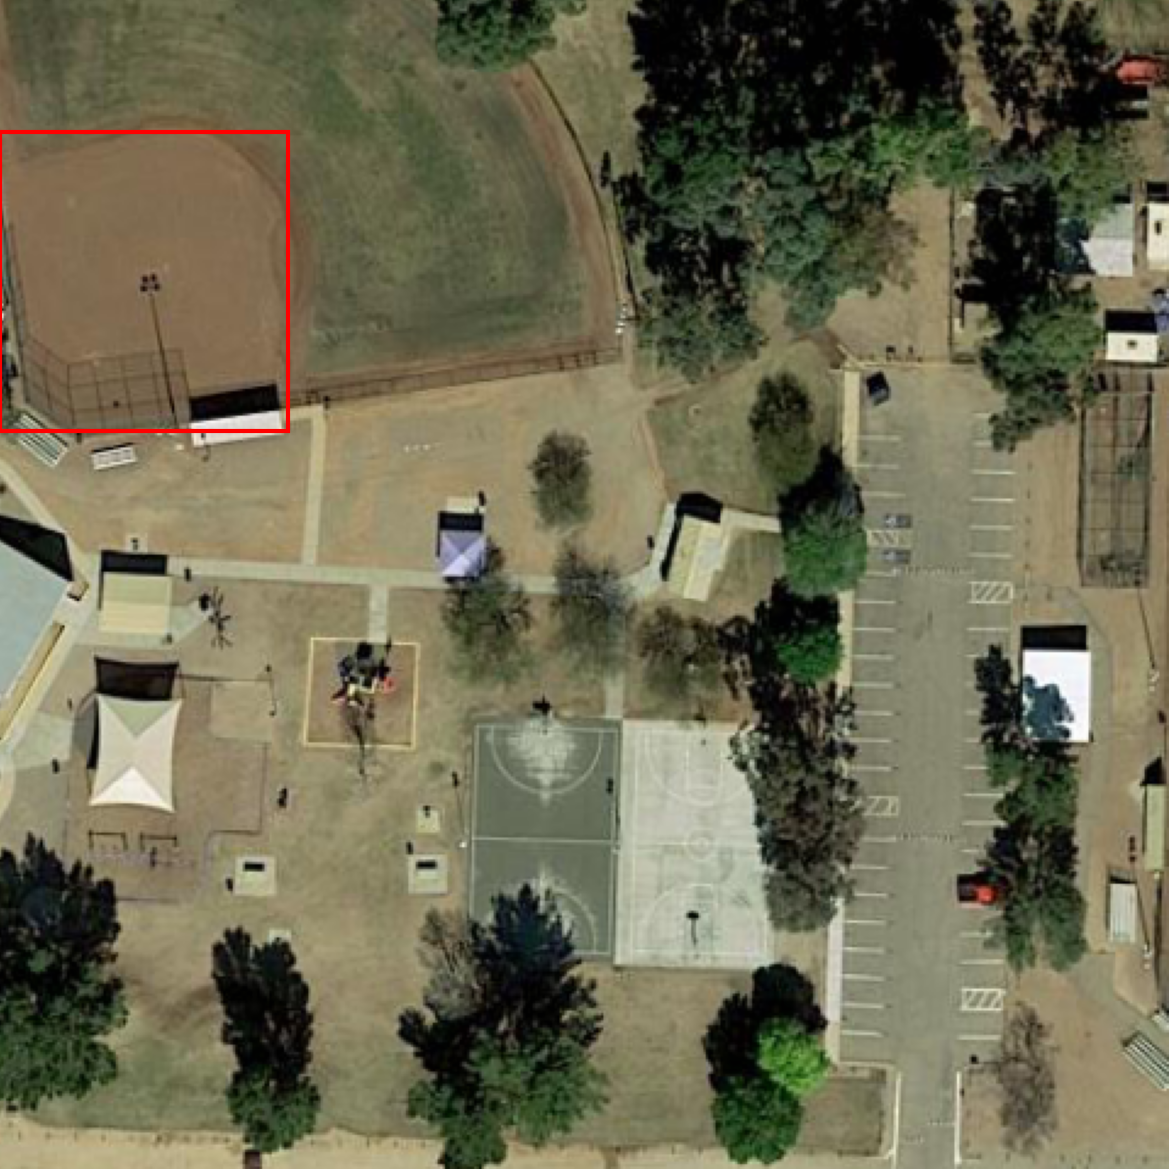
\includegraphics[width=0.65\textwidth]{Images/3llm.png}
\end{minipage}%
\begin{minipage}{0.5\textwidth}
\centering
\hspace{-1cm}
\raisebox{-0.3\height}{%
\footnotesize
\begin{tabular}{@{}p{2cm}p{5cm}@{}}
\toprule
\textbf{Expression Type} & \textbf{Example} \\
\midrule
Original & the orange baseball diamond in the top left \\
\midrule
o3 Enhanced & the orange baseball diamond with the light pole near home plate in the upper left \\
\midrule
Gemma3 Base & the bright orange baseball diamond to the left of another similar baseball diamond in the top left \\
\midrule
Gemma3-Aerial-12B & the orange baseball field with a chainlink fence surrounded by grass to the north and trees to the west \\
\bottomrule
\end{tabular}%
}
\end{minipage}
\caption{Qualitative comparison between o3, the base Gemma3 model, and the fine-tuned Gemma3-Aerial-12B model on aerial imagery. The sequence shows how each model enhances the original rule-based expression using the same prompt and decoding setup.}
\label{fig:distillation_comparison}
\end{figure*}

\begin{table}[t]
\centering
\caption{Cost analysis: Gemma3 vs. o3 model for large-scale annotation}
\label{tab:cost_comparison}
\begin{tabular}{@{}lcc@{}}
\toprule
\textbf{Model} & \textbf{Cost per request} & \textbf{Cost for 300K requests} \\
\midrule
o3 Model & \$0.020728 & \$6{,}218.32 \\
Distilled Gemma3 & \$0.000087 & \$26.01 \\
\midrule
\textbf{Savings} & \textbf{238× cheaper} & \textbf{\$6{,}192.31 (99.6\%)} \\
\bottomrule
\end{tabular}
\end{table}

The cost calculations are based on current API pricing: o3 costs \$2.00 per million input tokens and \$8.00 per million output tokens on the OpenAI API platform, while Gemma3-12B costs \$0.035 per million input tokens and \$0.141 per million output tokens through the OpenRouter inference provider. The average tokens per request are 1,670.8 input and 2,173.3 output for o3, compared to 1,330.0 input and 284.7 output for Gemma3, calculated based on 15 sample requests.

\subsection{Historic Filter Ablation Study}

Finally, we evaluate how much the historic-filter augmentation contributes to robustness by retraining the combined model without injecting filtered images. Models trained solely on clean, contemporary imagery often falter when archival photographs introduce monochrome toning, contrast loss, or sepia casts. Removing the filters exposes whether robustness stems from the augmentation or from dataset diversity alone.

Table~\ref{tab:historic_ablation_results} reports the outcome using the same metric format as the combined evaluation. Without filter injections the model gains a few points on the clean validation splits—for instance RRSIS-D climbs to 64.36\% mIoU—but it loses resilience on the historic versions. RefSegRS suffers the most, dropping from \textcolor{blue}{32.79\%} to \textcolor{blue}{27.73\%} mIoU and from \textcolor{blue}{36.74\%} to \textcolor{blue}{32.21\%} oIoU when confronted with filtered validation imagery. The Aerial-D and NWPU-Refer historic splits also shed several points, illustrating that the augmentation specifically protects datasets whose semantics depend on subtle colour and contrast cues.

These results confirm that modest exposure to historic degradations during training is enough to stabilise performance when evaluation imagery undergoes the same transformations. We therefore keep the filter injections in the final combined recipe despite the small trade-off in clean-split accuracy.

\begin{table}[H]
\centering
\caption{Historic filter ablation study—combined model trained on all datasets without historic-filter augmentation.}
\label{tab:historic_ablation_results}
\resizebox{\textwidth}{!}{%
\begin{tabular}{@{}lcccccccc@{}}
\toprule
\textbf{Dataset} & \textbf{IoU@0.5} & \textbf{IoU@0.7} & \textbf{IoU@0.9} & \multicolumn{2}{c}{\textbf{mIoU}} & \multicolumn{2}{c}{\textbf{oIoU}} \\
\cmidrule(lr){5-6} \cmidrule(lr){7-8}
 & & & & \textbf{Orig.} & \textbf{Hist.} & \textbf{Orig.} & \textbf{Hist.} \\
\midrule
Aerial-D & 59.48\% (\textcolor{red}{-0.62}) & 43.37\% (\textcolor{red}{-0.58}) & 12.60\% (\textcolor{red}{-0.45}) & 49.21\% (\textcolor{red}{-0.57}) & \textcolor{blue}{43.57\%} (\textcolor{red}{-3.25}) & 62.88\% (\textcolor{red}{-0.56}) & \textcolor{blue}{58.14\%} (\textcolor{red}{-2.98}) \\
RRSIS-D & 74.60\% (\textcolor{green!60!black}{+5.12}) & 58.39\% (\textcolor{green!60!black}{+4.77}) & 20.75\% (\textcolor{red}{-1.03}) & 64.36\% (\textcolor{green!60!black}{+2.66}) & \textcolor{blue}{59.02\%} (\textcolor{green!60!black}{+0.67}) & 75.59\% (\textcolor{green!60!black}{+2.15}) & \textcolor{blue}{72.50\%} (\textcolor{green!60!black}{+0.77}) \\
NWPU-Refer & 46.02\% (\textcolor{green!60!black}{+5.49}) & 32.32\% (\textcolor{green!60!black}{+4.67}) & 10.66\% (\textcolor{green!60!black}{+2.21}) & 41.06\% (\textcolor{green!60!black}{+3.17}) & \textcolor{blue}{33.42\%} (\textcolor{green!60!black}{+1.90}) & 58.35\% (\textcolor{green!60!black}{+7.01}) & \textcolor{blue}{53.04\%} (\textcolor{green!60!black}{+6.87}) \\
RefSegRS & 47.33\% (\textcolor{green!60!black}{+6.03}) & 13.23\% (\textcolor{green!60!black}{+4.18}) & 1.16\% (\textcolor{red}{-0.93}) & 41.31\% (\textcolor{green!60!black}{+1.21}) & \textcolor{blue}{27.73\%} (\textcolor{red}{-5.06}) & 50.30\% (\textcolor{green!60!black}{+5.25}) & \textcolor{blue}{32.21\%} (\textcolor{red}{-4.53}) \\
Urban1960SatSeg & 78.46\% (\textcolor{green!60!black}{+0.41}) & 60.98\% (\textcolor{green!60!black}{+1.02}) & 28.66\% (\textcolor{green!60!black}{+0.41}) & 69.81\% (\textcolor{green!60!black}{+0.46}) & N/A & 87.80\% (\textcolor{green!60!black}{+0.53}) & N/A \\
\bottomrule
\end{tabular}%
}
\end{table}

Collectively, the updated experiments demonstrate that the Aerial-D dataset, RSRefSeg backbone, and LLM-enhanced expressions form a cohesive system that generalises across aerial benchmarks, withstands historic degradations, and remains economically scalable. These results ground the dissertation's claims with the most recent evidence and align the thesis with the accompanying article.

% If Printing on DOUBLE SIDED pages, the second page should be white.
% Otherwise, comment the following command:
\cleardoublepage
%
%Chapter 6
% #############################################################################
% This is Chapter 6
% !TEX root = ../main.tex
% #############################################################################
% Change the Name of the Chapter i the following line
\fancychapter{Conclusion and Future Work}
\cleardoublepage
% The following line allows to ref this chapter
\label{chap:conclusion}

This thesis presents a comprehensive approach to open-vocabulary aerial image segmentation through the development of a complete dataset construction methodology and an effective model architecture. The work addresses the fundamental challenge of creating large-scale referring expression datasets for aerial imagery, where traditional manual annotation approaches prove prohibitively expensive and time-consuming.

To close the thesis, we first synthesize the main findings and contributions, and then outline forward-looking extensions and directions that build on this work.

% #############################################################################
\section{Conclusions}

This work introduces Aerial-D together with an end-to-end methodology that transforms existing aerial segmentation datasets into a comprehensive repository of referring expressions. The approach begins with a rule-driven generator that systematically converts instance masks into natural language descriptions by analyzing spatial location, visual appearance, and relational characteristics between objects. This foundation is then enhanced through a sophisticated pipeline that combines large language model rewriting with a distilled Gemma3 annotator~\cite{gemma3}, ensuring that the methodology remains both effective and computationally affordable.

The resulting dataset enables comprehensive training of the RSRefSeg architecture across five distinct benchmarks, demonstrating the robustness and generalizability of the approach. The experimental evaluation establishes new performance baselines on Aerial-D while achieving results that match or surpass previously published outcomes on established benchmarks including RRSIS-D, NWPU-Refer, RefSegRS, and Urban1960SatSeg~\cite{yuan2023rrsis,yang2024large,hao2025urban1960satseg}. These results validate both the quality of the generated dataset and the effectiveness of the proposed model architecture.

The systematic ablation studies conducted throughout this work provide valuable insights into the contributions of different components. The analysis of expression sources demonstrates how enhanced language descriptions translate into measurable improvements in model performance. Similarly, the evaluation of historic-image filters reveals how domain-specific augmentations contribute to increased robustness across different visual conditions and image characteristics.

The key contributions of this thesis can be summarized as follows: the development of the Aerial-D dataset through an innovative rule-based generation pipeline, the design of the RSRefSeg architecture that effectively combines SigLIP and SAM components for aerial image segmentation, the implementation of an LLM enhancement pipeline that scales high-quality expression generation, and the establishment of comprehensive evaluation protocols that demonstrate the effectiveness of the approach across multiple benchmarks.

% #############################################################################
\section{Future Work}

We identify three promising directions for future work, focusing on scalability, broader applicability, and technical advancement.

The first direction involves extending the expression-enhancement pipeline to existing public benchmarks. The methodology developed for Aerial-D can be directly applied to the native captions provided with established datasets such as RRSIS-D and NWPU-Refer. By enriching their existing language descriptions with the same visual grounding cues that proved effective for Aerial-D, it becomes possible to create a unified training pool with significantly higher linguistic variety. This approach would not only improve the quality of existing datasets but also enable more comprehensive cross-dataset training scenarios that could lead to improved generalization capabilities.

The second research direction focuses on multilingual expansion of the generated expressions. This can be achieved by integrating a production-grade language model such as OpenAI's o3~\cite{o3} with the established distillation pipeline. In this approach, the large language model would be responsible for drafting high-quality translations of the English expressions into multiple target languages, while the distilled Gemma3 student model would learn to reproduce these translations at scale. This methodology would preserve the domain-specific phrasing and technical accuracy that characterizes aerial imagery descriptions while producing a comprehensive multilingual corpus that could enable referring segmentation in diverse linguistic contexts.

The third and most ambitious direction involves leveraging emerging multimodal systems for synthetic data generation. Recent developments in multimodal artificial intelligence, such as Gemini 2.5~\cite{gemini25}, exhibit progressively stronger vision-language capabilities and controllable image generation. Integrating such systems into the established pipeline could enable the synthesis of new object classes paired with natural language expressions. These machine-generated samples could then be processed through the same rule-based expression generation stages developed in this work, potentially creating a pathway toward partially synthetic, open-vocabulary aerial datasets that supplement or extend real-world data collection efforts.
% If Printing on DOUBLE SIDED pages, the second page should be white.
% Otherwise, comment the following command:
\cleardoublepage
%
%Chapter 7
% #############################################################################
% This is Chapter 7
% !TEX root = ../main.tex
% #############################################################################
% Change the Name of the Chapter i the following line
\fancychapter{Conclusion and Future Work}
\cleardoublepage
% The following line allows to ref this chapter
\label{chap:conclusion}

Lorem ipsum dolor sit amet, consectetuer adipiscing elit. Morbi commodo, ipsum sed pharetra gravida, orci magna rhoncus neque, id pulvinar odio lorem non turpis. Nullam sit amet enim. Suspendisse id velit vitae ligula volutpat condimentum. Aliquam erat volutpat. Sed quis velit. Nulla facilisi. Nulla libero. Vivamus pharetra posuere sapien\todo[color=green!40, author=Rui Cruz, fancyline]{You should always start a Chapter with an introductory text}{}.

% #############################################################################
\section{Conclusions}
Lorem ipsum dolor sit amet, consectetuer adipiscing elit. Morbi commodo, ipsum sed pharetra gravida, orci magna rhoncus neque, id pulvinar odio lorem non turpis. Nullam sit amet enim. Suspendisse id velit vitae ligula volutpat condimentum. Aliquam erat volutpat. Sed quis velit. Nulla facilisi. Nulla libero. Vivamus pharetra posuere sapien. Nam consectetuer. Sed aliquam, nunc eget euismod ullamcorper, lectus nunc ullamcorper orci, fermentum bibendum enim nibh eget ipsum. Donec porttitor ligula eu dolor. Maecenas vitae nulla consequat libero cursus venenatis. Nam magna enim, accumsan eu, blandit sed, blandit a, eros.

\subsection{Main Contributions}
Quisque facilisis erat a dui. Nam malesuada ornare dolor. Cras gravida, diam sit amet rhoncus ornare, erat elit consectetuer erat, id egestas pede nibh eget odio. Proin tincidunt, velit vel porta elementum, magna diam molestie sapien, non aliquet massa pede eu diam. Aliquam iaculis. Fusce et ipsum et nulla tristique facilisis.

% #############################################################################
\section{Future Work}
Donec eget sem sit amet ligula viverra gravida. Etiam vehicula urna vel turpis. Suspendisse sagittis ante a urna. Morbi a est quis orci consequat rutrum. Nullam egestas feugiat felis. Integer adipiscing semper ligula. Nunc molestie, nisl sit amet cursus convallis, sapien lectus pretium metus, vitae pretium enim wisi id lectus. Donec vestibulum. Etiam vel nibh. Nulla facilisi. Mauris pharetra. Donec augue. Fusce ultrices, neque id dignissim ultrices, tellus mauris dictum elit, vel lacinia enim metus eu nunc.

\subsection{Immediate Extensions}
Proin at eros non eros adipiscing mollis. Donec semper turpis sed diam. Sed consequat ligula nec tortor. Integer eget sem. Ut vitae enim eu est vehicula gravida.

\subsection{Long-term Research Directions}
Morbi ipsum ipsum, porta nec, tempor id, auctor vitae, purus. Pellentesque neque. Nulla luctus erat vitae libero. Integer nec enim. Phasellus aliquam enim et tortor. Quisque aliquet, quam elementum condimentum feugiat, tellus odio consectetuer wisi, vel nonummy sem neque in elit. Curabitur eleifend wisi iaculis ipsum.
% If Printing on DOUBLE SIDED pages, the second page should be white.
% Otherwise, comment the following command:
\cleardoublepage
%
% -----------------------------------------------------------------------------
% BIBLIOGRAPHY
% Add the Bibliography to the PDF table of contents (not the document table of contents)
%\pdfbookmark[0]{Bibliography}{bib}
\addcontentsline{toc}{chapter}{Bibliography}
% The bibliography style sheet
% Chose your preferences on the format of the entries and the Labels:
% IEEEtran: Used in general (recommended for IST Thesis)
%           Entries are labelled and sorted by appearance in the document
%           Labels are Numeric inside square brackets
\bibliographystyle{IEEEtran}
%
% Apalike:  Entries formatted alphabetically, last name first, with identation
%           Labels with Autor's Name and Year inside square brackets
%\bibliographystyle{apalike}
%
% Alpha:    Entries formatted with Autor's Name and Year, hanging identation
%           Labels with Autor's abbr. Names and Year inside square brackets
%\bibliographystyle{alpha}
%
% Acm:     Entries formatted with Autor's Name (small Caps), hanging identation
%          Labels are Numeric inside square brackets
%\bibliographystyle{acm}
% The following command resets the 'emphasis' style for bibliography entries
\normalem
% Name of your BiBTeX file
\bibliography{./Thesis-MSc-Bibliography} % Put here your own filename
%
% The following command modifies the 'emphasis' style for bibliography entries
\ULforem
% If Printing on DOUBLE SIDED pages, the second page should be white.
% Otherwise, comment the following command:
\cleardoublepage
%
% -----------------------------------------------------------------------------
% HERE GO THE APPENDIXES IF REQUIRED
% If not required just comment the blocks
\appendix
%% First Appendix
%\pdfbookmark[1]{Appendix A}{appendix}
% #############################################################################
% This is Appendix A
% !TEX root = ../main.tex
% #############################################################################
\chapter{LLM Enhancement Prompts}
\label{chapter:appendixA}

This appendix contains the complete set of prompts used for enhancing referring expressions with Large Language Models in the AerialSeg dataset generation pipeline.

\section{Gemma3 Enhancement Prompts}

[LLM prompts for Gemma3-based expression enhancement to be added here - including system prompts, user prompts, and examples used for generating natural language variations of rule-based referring expressions]

\section{OpenAI O3 Enhancement Prompts}

[LLM prompts for OpenAI O3-based expression enhancement to be added here - including prompts for visual detail generation and linguistic diversity improvements]

\section{Fine-tuning Prompts}

[Prompts used for LoRA fine-tuning of Gemma3 model to be added here - including training examples and task-specific instructions for aerial image referring expression generation]
%% If Printing on DOUBLE SIDED pages, the second page should be white.
%% Otherwise, comment the following command:
\cleardoublepage
%% Second Appendix - Removed (was template content)

% -----------------------------------------------------------------------------
% And this is THE END of the IST Thesis Document
\end{document}